%
% Niniejszy plik stanowi przyk�ad formatowania pracy magisterskiej na
% Wydziale MIM UW.  Szkielet u�ytych polece� mo�na wykorzystywa� do
% woli, np. formatujac wlasna prace.
%
% Zawartosc merytoryczna stanowi oryginalnosiagniecie
% naukowosciowe Marcina Wolinskiego.  Wszelkie prawa zastrze�one.
%
% Copyright (c) 2001 by Marcin Woli�ski <M.Wolinski@gust.org.pl>
% Poprawki spowodowane zmianami przepis�w - Marcin Szczuka, 1.10.2004
% Poprawki spowodowane zmianami przepisow i ujednolicenie 
% - Seweryn Kar�owicz, 05.05.2006
% dodaj opcj� [licencjacka] dla pracy licencjackiej
\documentclass{pracamgr}
\usepackage{amsmath}
\usepackage{amsfonts}
\usepackage[a4paper, left=2.5cm, right=2.5cm, top=3.5cm, bottom=3.5cm, headsep=1.2cm]{geometry}
\usepackage{graphicx}
\usepackage{float}
\usepackage{enumerate}
\usepackage{ mathrsfs }
\usepackage{ amssymb }
\usepackage{amsthm}
\usepackage{etoolbox}
\usepackage{ dsfont }
\usepackage{ hyperref }
\usepackage{mathtools}
\usepackage{pdfpages}
%\usepackage{standalone}

%Jesli uzywasz kodowania polskich znakow ISO-8859-2 nastepna linia powinna byc 
%odkomentowana
%\usepackage[latin2]{inputenc}
%Jesli uzywasz kodowania polskich znakow CP-1250 to ta linia powinna byc 
%odkomentowana
\usepackage[cp1250]{inputenc}



% Dane magistranta:

\author{Adam �piewak}

\nralbumu{132528}

\title{Generalizations of Wiener-Wintner ergodic theorem}

\tytulang{Rozszerzenia twierdzenia ergodycznego Wienera-Wintnera}

%kierunek: Matematyka, Informatyka, ...
\kierunek{Matematyka}

% informatyka - nie okreslamy zakresu (opcja zakomentowana)
% matematyka - zakres moze pozostac nieokreslony,
% a jesli ma byc okreslony dla pracy mgr,
% to przyjmuje jedna z wartosci:
% {metod matematycznych w finansach}
% {metod matematycznych w ubezpieczeniach}
% {matematyki stosowanej}
% {nauczania matematyki}
% Dla pracy licencjackiej mamy natomiast
% mozliwosc wpisania takiej wartosci zakresu:
% {Jednoczesnych Studiow Ekonomiczno--Matematycznych}

% \zakres{Tu wpisac, jesli trzeba, jedna z opcji podanych wyzej}

% Praca wykonana pod kierunkiem:
% (poda� tytu�/stopie� imi� i nazwisko opiekuna
% Instytut
% ew. Wydzia� ew. Uczelnia (je�eli nie MIM UW))
\opiekun{prof. dra hab. in�. Wojciecha Bartoszka\\
  Katedra Rachunku Prawdopodobie�stwa i Biomatematyki\\
  }

% miesi�c i~rok:
\date{Czerwiec 2015}

%Poda� dziedzin� wg klasyfikacji Socrates-Erasmus:
\dziedzina{ 
%11.0 Matematyka, Informatyka:\\ 
11.1 Matematyka\\ 
%11.2 Statystyka\\ 
%11.3 Informatyka\\ 
%11.4 Sztuczna inteligencja\\ 
%11.5 Nauki aktuarialne\\
%11.9 Inne nauki matematyczne i informatyczne
}

%Klasyfikacja tematyczna wedlug AMS (matematyka) lub ACM (informatyka)
\klasyfikacja{37 Dynamical systems and ergodic theory\\
  37A Ergodic theory\\
  37A30 Ergodic theorems, spectral theory, Markov operators}

% S�owa kluczowe:
\keywords{teoria ergodyczna}

% Tu jest dobre miejsce na Twoje w�asne makra i~�rodowiska:
\newtheoremstyle{dotless}{}{}{}{}{\bfseries}{}{ }{}
\newtheoremstyle{withspace}{}{}{}{}{\bfseries}{ }{ }{}
\newtheoremstyle{colon}{0}{}{}{}{\bfseries}{:}{ }{}

\newtheoremstyle{mytheorem}%                % Name
  {}%                                     % Space above
  {}%                                     % Space below
  {\itshape}%                             % Body font
  {}%                                     % Indent amount
  {\bfseries}%                            % Theorem head font
  {}%                                    % Punctuation after theorem head
  {\newline}%                                    % Space after theorem head, ' ', or \newline
  {}%                                     % Theorem head spec (can be left empty, meaning `normal')


\newtheoremstyle{fact}%                % Name
  {}%                                     % Space above
  {}%                                     % Space below
  {\itshape}%                             % Body font
  {}%                                     % Indent amount
  {\bfseries}%                            % Theorem head font
  {}%                                    % Punctuation after theorem head
  { }%                                    % Space after theorem head, ' ', or \newline
  {}%                                     % Theorem head spec (can be left empty, meaning `normal')


\theoremstyle{mytheorem}
\newtheorem{thm}{Theorem}[chapter]
\newtheorem{lem}{Lemma}[chapter]
\newtheorem{cor}{Corollary}[chapter]
\newtheorem{prop}{Proposition}[chapter]

\theoremstyle{fact}
\newtheorem{f}{Fact}[chapter]

\theoremstyle{withspace}
\newtheorem{df}{Definition}[chapter]
\newtheorem{ex}{Example}[chapter]

\theoremstyle{dotless}
\newtheorem*{rem}{Remark}


\theoremstyle{colon}
\newtheorem*{pf}{Proof}

\AfterEndEnvironment{thm}{\noindent\ignorespaces}
\AfterEndEnvironment{lem}{\noindent\ignorespaces}
\AfterEndEnvironment{df}{\noindent\ignorespaces}
\AfterEndEnvironment{prop}{\noindent\ignorespaces}
\AfterEndEnvironment{ex}{\noindent\ignorespaces}
\AfterEndEnvironment{rem}{\noindent\ignorespaces}
\AfterEndEnvironment{pf}{\noindent\ignorespaces}
\AfterEndEnvironment{f}{\noindent\ignorespaces}

% koniec definicji


\begin{document}
\maketitle

%tu idzie streszczenie na strone poczatkowa
\begin{abstract}
The Wiener-Wintner ergodic theorem (\ref{t:ww}) states that for a given ergodic dynamical system $(X, \mathcal{A}, \mu, T)$ and fixed $f \in L^1(\mu)$ there exists a set of full measure $X_f$ such that $\lim \limits_{N \rightarrow \infty} \frac{1}{N} \sum \limits_{n=0}^{N-1} \lambda^n f (T^n x )$ exists for every $x \in X_f$ and $\lambda$ from the unit circle $\mathbb{T}$ on the complex plane. We state and prove several generalizations of this theorem. Bourgain's theorem (\ref{t:bourgain}) establishes uniform convergence with respect to $\lambda \in \mathbb{T}$ and Robinson's theorem (\ref{t:robinson}) gives uniform convergence with respect to $x \in X$ in the case of uniquely ergodic topological systems (under suitable additional assumptions). Schreiber's theorem (\ref{t:schreiber}) gives a condition equivalent to the mean ergodicity of distorted semigroup $\{\chi(g)S_g : g \in G \}$ for a given uniquely ergodic Markovian representation $\mathcal{S}$ of an amenable semitopological semigroup $G$ on $C(X)$ and continuous character $\chi: G \rightarrow \mathbb{T}$. This can be seen as a natural extension of Robinson's theorem to the abstract semigroup case. We finish the thesis with generalization of Schreiber's theorem to the case of mean ergodic semigroup $\mathcal{S}$ (\ref{t:markov_ww}) with finite dimensional fixed space $Fix(\mathcal{S})$ (\ref{t:finite_dim_markov_ww}), giving simultaneously more elementary proof. We give also version of the theorem characterizing convergence of the ergodic nets for the single function $f \in C(X)$ (\ref{t:single_markov_ww}). We present also necessary framework from measure theory, functional analysis, spectral theory for isometries on Hilbert spaces, Markov operators and ergodic theory for deterministic transformations and operator semigroups.
\newpage
\end{abstract}

\tableofcontents
%\listoffigures
%\listoftables

\chapter*{Introduction}

The classical result of ergodic theory is the Birkhoff's ergodic theorem. It states, that for an ergodic dynamical system $(X, \mathcal{A},\mu, T)$ and $f \in L^1(\mu)$ there is $\lim \limits_{N \rightarrow \infty} \sum \limits_{n=0}^{N} f(T^nx) = \int \limits_X f d\mu\ \mu$-a.e. The Wiener-Wintner ergodic theorem deals with the convergence of distorted Ceasaro averages $\frac{1}{N} \sum \limits_{n=0}^{N-1} \lambda^n f(T^n x)$ for $\lambda \in \mathbb{T}:=\{ z \in \mathbb{C}: |z| = 1 \}$. The result of N. Wiener and A. Wintner from 1941 (\cite{ww}) states that if the system is ergodic then for every $f \in L^1(\mu)$ there exsists a measurable set of full measure $X_f$ such that $\lim \limits_{N \rightarrow \infty} \frac{1}{N} \sum \limits_{n=0}^{N-1} \lambda^n f (T^n x )$ exists for every $x \in X_f$ and every $\lambda \in \mathbb{T}$. This thesis investigates several generalizations of this result.\\

Chapter 1. introduces notation and gives necessary preliminaries from measure  theory, topology, functional analysis and spectral theory for isometries on Hilbert spaces. Proof are contained only in the last section.\\

Chapter 2. gives brief introduction to the ergodic theory for measure preserving and topological dynamical systems.\\

Chapter 3. is the first main chapter of the thesis. We prove Wiener-Wintner theorem and give two other Wiener-Wintner type theorems. Both of them deal with the uniform convergence of the distorted averages. Bourgain's uniform Wiener-Wintner theorem (\cite{bourgain}, 1990) states that for a function $f \in L^2(\mu)$ which is orthogonal to the Kronecker factor of the system there is $\lim \limits_{N \rightarrow \infty}\  \sup \limits_{\lambda \in \mathbb{T}}\ \left| \frac{1}{N} \sum \limits_{n=0}^{N-1} \lambda^n f(T^n x) \right| = 0.$ Robinson's topological Wiener-Wintner theorem (\cite{robinson}, 1994) gives condtion under which for a uniquely ergodic topological system $(X,T)$ and fixed $\lambda \in \mathbb{T}$ the sequence $\frac{1}{N}\sum \limits_{n=0}^{N} \lambda^n f \circ T^n$ converges in $C(X)$ for every $f \in C(X)$. We prove also reverse theorems. The proofs are based on the spectral theory. Wide treatment of these issues can be found in the book \cite{assani}.\\

Chapter 4. contains introduction to the ergodic theory for operator semigroups. We consider bounded representations of semitopological semigroups on Banach spaces. We introduce the concept of ergodic net, which is a generalization of the sequence of the Ceasaro averages. Following M. Schreiber in \cite{schreiber13} and \cite{schreiber14}, we state the Abstract mean ergodic theorem in this language. We introduce concepts of the amenable semigroups and Markov operators on $C(X)$, where $X$ is a compact Hausdorff topological space. We state and prove several properties of the latter.\\

Chapter 5. is the second main chapter of the thesis. It is based on the article \cite{schreiber14}, which includes characterization of the mean ergodicity of the semigroup $_{\chi}\mathcal{S}:=\{ \chi(g)S_g: g \in G \}$, where $\mathcal{S}=\{S_g: g \in G \}$ is a uniquely ergodic bounded Markovian representation of (right) amenable semigroup $G$ on $C(X)$ and $\chi:G \rightarrow \mathbb{T}$ is a continous semigroup homomorphism (character). This thesis consists results from the unpublished yet paper \cite{bartoszek}, which generalizes Schreiber's results to the case of mean (not necessarily uniquely) ergodic Markovian representations. We generalize also Schreiber's result on the convergence of an $_{\chi}\mathcal{S}$-ergodic net on a single function $f \in C(X)$ to the case of the arbitrary bounded Markovian representation $\mathcal{S}$ on $C(X)$.\\
\addcontentsline{toc}{chapter}{Introduction}
%%% Local Variables:
%%% mode: latex
%%% TeX-master: t
%%% coding: latin-2
%%% End:






\chapter{Preliminaries}\label{r:prel}
In this chapter we introduce basic notations, concepts and theorems from measure theory, topology, functional analysis and spectral theory for isometries on Hilbert spaces which will be used through the thesis. We omit most of the proofs.\\ \\
By $\mathbb{N}$ we will denote set of positive natural numbers, by $\mathbb{N}_0$ - set of natural numbers with zero, by $\mathbb{Z}$ - set of integers, by $\mathbb{R}$ - set of real numbers, by $\mathbb{C}$ - set of complex numbers and by $\mathbb{T}=\mathbb{S}^1=\left\{ \lambda \in \mathbb{C}: |\lambda|=1 \right\}$ - circle on a complex plane (1-dimensional torus).



\section{Measure theory}
By $(X, \mathcal{A}, \mu)$ we will denote a measure space, where $X$ is a nonempty set, $\mathcal{A}$ is a $\sigma$-field of subsets of $X$ and $\mu$ is a measure on the measurable space $(X, \mathcal{A})$. By term 'measure' we will always mean a $\sigma$-additive, non-negative measure. When we will wish measure $\mu$ to have complex values we will introduce it as a 'complex measure $\mu$'. Sets $A \in \mathcal{A}$ are called measurable sets. Measure $\mu$ is called finite if $\mu(X) < \infty$ and $\sigma$-finite if there is a countable collection of measurable sets $\{ A_n \}_{n=1}^{\infty}$ with $\mu(A_n)<\infty$ for each $n \in \mathbb{N}$, such that $X = \bigcup \limits_{n=1}^{\infty} A_n$. If measure $\mu$ is $\sigma$-finite, then the sets $\{ A_n \}_{n=1}^{\infty}$ can be taken to be pairwise disjoint. If $\mu(X)=1$ then the measure $\mu$ is called a probability measure and $(X, \mathcal{A}, \mu)$ is called a probability space. For a finite measure $\mu$, set $A \in \mathcal{A}$ is said to have a full measure if $\mu(A) = \mu (X)$. We will often use the following simple

\begin{f} Let $(X, \mathcal{A}, \mu)$ be a measure space with a finite measure and take measurable sets $A_n, n \in \mathbb{N}$. If each $A_n$ has a full measure, then their intesection $\bigcap \limits_{n=1}^{\infty} A_n$ also has a full measure.
\end{f}

\begin{df}
Let $(X, \mathcal{A})$ and $(Y, \mathcal{C})$ be measurable spaces. A map $T: X \rightarrow Y$ is called a \textbf{measurable map} if it satisfies $T^{-1}(C) \in \mathcal{A} \text{ for all } C \in \mathcal{C}$.
\end{df}

\begin{df}
Let $(X, \mathcal{A}, \mu)$ be a measure space. An element $x \in X$ is called an \textbf{atom} (of the measure $\mu$) if $\mu(\{ x\})>0$. The measure $\mu$ is called \textbf{continuous} if it has no atoms, i.e. $\underset{x \in X}{\forall}\ \mu(\{ x\})=0$.
\end{df}

\begin{rem} Note that a finite measure $\mu$ can have only countably many atoms. To see that observe that for $\varepsilon >0$ a set $A_{\varepsilon}:=\{x \in X: \mu(\{x\}) > \epsilon \}$ must have at most $\frac{\mu(X)}{\varepsilon}$ elements (otherwise we wolud have $\mu(X) > \frac{\mu(X)}{\varepsilon} \cdot \varepsilon = \mu(X)$), hence must be finite. This shows that the set of atoms $A = \bigcup \limits_{n=1}^{\infty} A_{\frac{1}{n}}$ must be countable. Also, there is $\sum \limits_{x \in A} \mu(\{ x\}) \leq \mu(X) < \infty.$
\end{rem}
If $X$ is a topological space, then by $\mathcal{B}(X)$ we will denote its Borel $\sigma$-field, i.e. the smallest $\sigma$-field containing all open subsets of $X$. Note that if $X$ and $Y$ are topological spaces and $T:X \rightarrow Y$ is continuous, then T is also measurable (with respect to Borel $\sigma$-fields on $X$ and $Y$). Measure on a measurable space $(X, \mathcal{B}(X))$ is called a Borel measure. On spaces $\mathbb{R}^n, n \in \mathbb{N}$ (with a standard topology) there is a natural Borel measure, which is a unique measure $m$ with property $m([a_1, b_1]\times [a_2, b_2] \times ... \times [a_n, b_n]) = (b_1 - a_1)(b_2 - a_2)...(b_n - a_n)$ for $a_1\leq b_1,a_1\leq b_2, ..., a_n\leq b_n$. This measure $m$ is called a Lebesgue measure and it's $\sigma$-finite. On $\mathbb{T}$ (with a standard topology) there exists a unique measure such that measure of any arc is its length. This measure is finite and its normalization will be also called a Lebesgue measure and will be denoted by $m$ ($m(\mathbb{T})=1$ and length of arc $A$ is equal to $2\pi m(A)$).\\ \\
Let $T, S: X \rightarrow Y$ be a measurable maps between measurable spaces $(X, \mathcal{A})$ and $(Y, \mathcal{C})$. We will use abreviations $\{ T \in A \}:= \{x \in X: Tx \in A \}$, $\{ T=S \} := \{x \in X: Tx = Sx \}$ and $\{ T \neq S \} := \{x \in X: Tx \neq Sx \}$. Note that these set are measurable. We will say that some property holds for ($\mu$) almost all $x \in X$, if there is a measurable set $A$ such that this property holds for every $x \in A$ and $\mu(X \backslash A) = 0$. We will say that map $T$ is equal to $S$ $\mu$ almost everywhere ($\mu$-a.e.) if $Tx = Sx$ for almost all $x \in X$, i.e. $\mu(T \neq S):=\mu(\{T \neq S\})=0$.\\ \\
We say that function $f:X \rightarrow \mathbb{R}^n$ or $f:X \rightarrow \mathbb{C}^n$ is a Borel function (or simply a measurable function) if it is measurable with respect to the Borel $\sigma$-field $\mathcal{B}(\mathbb{R}^n)$ or $\mathcal{B}(\mathbb{C}^n)$, where we consider the standard topology on $\mathbb{R}^n$ or $\mathbb{C}^n$. Let $(f_n)_{n \in \mathbb{N}}$ be  a sequence of measurable complex-valued functions on $X$. We say that the sequence $(f_n)_{n \in \mathbb{N}}$ converges $\mu$ almost everywhere to a measurable function $f: X \rightarrow \mathbb{C}$ if $\lim \limits_{n \rightarrow \infty} f_n(x) = f(x)$ for almost all $x \in X$. The following important theorem says when a.e. convergence implies convergence of integrals.
\begin{thm}[Lebesgue Dominated Convergence Theorem]
Let $(X, \mathcal{A}, \mu)$ be a measure space and let $f, f_1, f_2, ...$ be a sequence of measurable, complex-valued functions on $X$ with $f_n \stackrel{n \rightarrow \infty}{\longrightarrow} f\ \mu$-a.e. Suppose further, that there is a measurable function $g: X \rightarrow [0, \infty)$ with $|f_n| \leq g\ \mu$-a.e. for every $n \in \mathbb{N}$ and $\int \limits_X gd\mu < \infty$. Then functions $f, f_1, f_2, ...$ are integrable and
\[ \lim \limits_{n \rightarrow \infty} \int \limits_{X} f_n d\mu = \int \limits_{X} f d\mu. \]
\end{thm}
Given two measure spaces $(X, \mathcal{A}, \mu)$ and $(Y, \mathcal{C}, \nu)$ there is a natural measurable structure on the product $X \times Y$. We define product $\sigma$-field $\mathcal{A} \otimes \mathcal{C}$ of the subsets of $X \times Y$ as the smallest $\sigma$-field containing all measurable rectangles $A\times C, A\in \mathcal{A}, C \in \mathcal{C}$, i.e. $\mathcal{A} \otimes \mathcal{C}:= \sigma( \{A \times C:  A\in \mathcal{A}, C \in \mathcal{C}\})$. Moreover, if both measures $\mu$ and $\nu$ are $\sigma$-finite, then there exists unique measure $\mu \otimes \nu$ on the measurable space $(X \times Y, \mathcal{A} \otimes \mathcal{C})$ with the property $\mu \otimes \nu (A \times C) = \mu(A)\nu(C)$ for all $A \in \mathcal{A}, C \in \mathcal{C}$. The measure $\mu \otimes \nu$ is called a product measure. Fubini's theorem establishes connection between integral with respect to the product measure and iterated integrals with respect to the measures $\mu$ and $\nu$ separately.
\begin{thm}[Fubini's Theorem]
Let $(X, \mathcal{A}, \mu)$ and $(Y, \mathcal{C}, \nu)$ be measure spaces with $\sigma$-finite measures. Let $f:X\times Y \rightarrow \mathbb{C}$ be measurable with respect to the product $\sigma$-field $\mathcal{A} \otimes \mathcal{C}$ and suppose that at least one of the following integrals is finite:
\[ \int \limits_{X \times Y} |f|d\mu \otimes \nu,\ \int \limits_{X} \left( \int \limits_{Y} |f(x,y)| d\nu(y) \right) d\mu(x),\ \int \limits_{Y} \left( \int \limits_{X} |f(x,y)| d\mu(x) \right) d\nu(y).\]
Then for $\mu$-almost all $x \in X$ the function $f(x, \cdot) : Y \rightarrow \mathbb{C}$ is $\nu$-finitely integrable and for $\nu$-almost all $y \in Y$ the function $f(\cdot, y) :X \rightarrow \mathbb{C}$ is $\mu$-finitely integrable. Moreover function $X \ni x \mapsto \int \limits_{Y} f(x, y) d\nu(y) \in \mathbb{C}$ is $\mu$-finitely integrable and function $Y \ni y \mapsto \int \limits_{Y} f(x, y) d\mu(x) \in \mathbb{C}$ is $\nu$-finitely integrable. The following equality holds:
\[ \int \limits_{X \times Y} fd\mu \otimes \nu = \int \limits_{X} \left( \int \limits_{Y} f(x,y) d\nu(y) \right) d\mu(x) = \int \limits_{Y} \left( \int \limits_{X} f(x,y) d\mu(x) \right) d\nu(y).\]
\end{thm}
\begin{rem} Note that functions $X \ni x \mapsto \int \limits_{Y} f(x, y) d\nu(y) \in \mathbb{C}$ and $Y \ni y \mapsto \int \limits_{Y} f(x, y) d\mu(x) \in \mathbb{C}$ may not be defined properly for every $x \in X$ and $y \in Y$, although they are definied $\mu$- and $\nu$-almost everywhere, which is enough to define properly their integrals.
\end{rem}
There is also a version of Fubini's Theorem for non-negative functions. In this case the integrals do not need to be finite.
\begin{thm}[Fubini's Theorem for non-negative functions]
Let $(X, \mathcal{A}, \mu)$ and $(Y, \mathcal{C}, \nu)$ be measure spaces with $\sigma$-finite measures. Let $f:X\times Y \rightarrow [0, \infty)$ be measurable with respect to the product $\sigma$-field $\mathcal{A} \otimes \mathcal{C}$. Then  function $X \ni x \mapsto \int \limits_{Y} f(x, y) d\nu(y) \in \mathbb{C}$ is $\mathcal{A}$-measurable and function $Y \ni y \mapsto \int \limits_{Y} f(x, y) d\mu(x) \in \mathbb{C}$ is $\mathcal{C}$-measurable and the following equality holds:
\[ \int \limits_{X \times Y} fd\mu \otimes \nu = \int \limits_{X} \left( \int \limits_{Y} f(x,y) d\nu(y) \right) d\mu(x) = \int \limits_{Y} \left( \int \limits_{X} f(x,y) d\mu(x) \right) d\nu(y).\]
\end{thm}
\begin{rem} Note that these integrals may be infinite and if at least one of them is infinite, then all of them are. \end{rem}

\begin{df}
Let $X$ be a compact topological space and let $\mu$ be a finite, non-negative Borel measure on $X$. We say that $\mu$ is \textbf{regular} if
\begin{enumerate}[(i)]
\item for every $A \in \mathcal{B}(X)$ there is $\mu(A) = \inf\{\mu(U): A \subset U, U \text{ is open} \}$,
\item for every $A \in \mathcal{B}(X)$ there is $\mu(A) = \sup\{\mu(K): K \subset A, K \text{ is compact} \}$.
\end{enumerate}
\end{df}

\begin{df}\label{d:measuremodulus}
Let $\mu$ be a complex measure on a measurable space $(X, \mathcal{A})$. We define its total variation measure $| \mu|$ as a non-negative measure on  $(X, \mathcal{A})$ given by
\[ |\mu| (A) := \sup \{ \sum \limits_{j=1}^{\infty} |\mu (E_j ) | : E_1, E_2, ... \text{ are pairwise disjoint and } \bigcup \limits_{j=1}^{\infty} E_j = A \}. \]
\end{df}
$| \mu |$ is always a finite measure (note that a complex measure, unlike the non-negative or signed measure, cannot attain values $+\infty$ or $- \infty$ by definition). For every $A \in \mathcal{A}$ there is $| \mu(A) | \leq |\mu|(A)$ and $| \mu(A) | = |\mu|(A)$ does not hold in general. We say that complex Borel measure is regular if its total variation measure is regular.

\section{Functional analysis}
We will always assume that vector spaces are taken over field $\mathbb{C}$. By $\| \cdot \|$ we will denote a norm of a normed space. We will give now standard examples of Banach spaces (i.e. complete normed space) with their properties which will be useful for us later.

\begin{ex}[$\mathscr{L}^p$ and $L^p$ spaces]$\\$
Let $(X, \mathcal{A}, \mu)$ be a measure space. For $1\leq p < \infty$ consider the vector space \[\mathscr{L}^p(X, \mathcal{A}, \mu) := \left\{ f:X \rightarrow \mathbb{C};\ f \text{ is measurable and } \int \limits_{X} |f|^p d\mu < \infty \right\}.\]
Define an equivalence relation $\sim$ on $\mathscr{L}^p(X, \mathcal{A}, \mu)$ by $f \sim g$ if $f = g\ \mu$ a.e. Let
\[ L^p(X, \mathcal{A}, \mu) := \mathscr{L}^p(X, \mathcal{A}, \mu) / \sim. \]
Space $L^p(X, \mathcal{A}, \mu)$ endowed with the norm $\|f\|_{L^p(X, \mathcal{A}, \mu)} :=  \left( \int \limits_{X} |f|^p d\mu \right) ^ {\frac{1}{p}}$ become Banach spaces. Usually we will abbreviate $L^p(X, \mathcal{A}, \mu)$ to $L^p(\mu)$ or $L^p$ and $\|\cdot\|_{L^p(X, \mathcal{A}, \mu)}$ to $\| \cdot \|_{L^p(\mu)}$ or $\|\cdot\|_p$.
\end{ex}

\begin{prop}
Let $(X, \mathcal{A}, \mu)$ be a measure space with a finite measure. Then for $1 \leq p < q < \infty$ we have $\mathscr{L}^q (\mu) \subset \mathscr{L}^p(\mu)$ and $L^q(\mu)$ is dense in $L^p(\mu)$ (in $L^p$ norm).
\end{prop}

\begin{ex}[Space $C(X)$]\label{ex:lp}$\\$
Let $X$ be a compact topological space (we assume that comapct spaces are Hausdorff by definition). Denote by $C(X)$ set of all complex valued continuous functions on $X$. $C(X)$ is a Banach space with norm $\|f\|_{\text{sup}} := \sup \limits_{x \in X} |f(x)|,\ f \in C(X)$. $C(X)$ is separable if and only if $X$ is metrizable (\cite[thm. 4.7]{eisner}). Suppose that there is a finite Borel nonegative measure $\mu$ on $X$. Any function $f \in C(X)$ is bounded, hence integrable with any power $p \in [1, \infty)$, what means that $C(X) \subset \mathscr{L}^p(\mu)$ and $C(X)$ can be embedded into $L^p(X, \mathcal{B}(X), \mu)$. Therefore, space $C(X)$ can be naturally seen as a linear subspace of space $L^p(\mu)$ (with identification of functions equal $\mu$ a.e., so equivalence class $f \in L^2(\mu)$ is also in the subspace $C(X)$ if it has continuous representative).
\end{ex}

\begin{prop}
Let $X$ be a compact topological space and $\mu$ be a finite nonegative Borel measure on $X$. Then $C(X)$ is dense in $L^p(\mu)$ (in $L^p$ norm) for every $p \in [1, \infty)$.
\end{prop}
By $\langle \cdot,\cdot \rangle$ we will denote inner product on a inner product space. Inner product space is also a normed space with a norm $\|x\| := \sqrt{\langle x, x \rangle}$. If inner product space is complete with this norm, we call it a Hilbert space.

\begin{ex}[Space $L^2(\mu)$]$\\$
Let $(X, \mathcal{A}, \mu)$ be a measure space. The space $L^2(\mu)$ with inner product $\langle f,g\rangle := \int \limits_{X} f \overline{g} d\mu$ is a Hilbert space. Note that the inner product norm coincides with norm $\| \cdot \|_{L^2(\mu)}$ from Example \ref{ex:lp}.
\end{ex}

\begin{prop}[Cauchy�Schwarz inequality]$\\$
Let $H$ be an inner product space. The following inequality holds for all $x,y \in H$:
\[ |\langle x, y \rangle | \leq \|x\| \|y\|. \]
\end{prop}

%\begin{rem} Cauchy-Schwarz inequality implies that inner product is a continous map in each variable.
%\end{rem}

\begin{df}
Let $H$ be an inner product space. Two vectors $x, y \in H$ are said to be \textbf{orthogonal} if $\langle x, y \rangle = 0$ (we write $x \bot y$). For a set $H_0 \subset H$ its \textbf{orthogonal complement} is a set $H_0^{\bot}:=\left\{ x \in H: \underset{h \in H_0}{\forall}\ \langle h, x \rangle = 0 \right\}$.
\end{df}

\begin{rem} If $H_0$ is a linear subspace of H, then $H_0^{\bot}$ is a closed linear subspace of H.
\end{rem}

\begin{df}
Let $E, F$ be normed spaces. A linear transformation $U: E \rightarrow F$ is called a \textbf{bounded linear operator} if there exists $M > 0$ such that $\underset{x \in E}{\forall}\ \|Ux\| \leq M\|x\|$. The constant $\|U\| := \sup \limits_{\|x\| \leq 1} \|Ux\|$ is called a \textbf{operator norm} of U. If $\| U \| \leq 1$ then $U$ is called a \textbf{contraction}. If $\underset{x \in E}{\forall}\ \|Ux\| = \|x\|$ then $U$ is called an \textbf{isometry}. Note that an isometry is always a contraction.
\end{df}

\begin{rem} Linear operator $U: E \rightarrow F$ between normed spaces is continuous if and only if it's bounded. The space $L(E,F)$ of all bounded linear operators, endowed with the operator norm is a normed space. $L(E,F)$ is a Banach space if and only if $F$ is a Banach space.
\end{rem}

\begin{df}
Let $E$ be a normed space and let $U:E \rightarrow E$ be a (bounded) linear operator. Number $\lambda \in \mathbb{C}$ is called an \textbf{eigenvalue} if there is a vector $x \in E,\ x \neq 0$ such that $Ux = \lambda x$. Any such a vector $x$ is called an \textbf{eigenvector} (associated with $\lambda$). The closed linear subspace $H_{\lambda} = \left\{ x \in H: Ux = \lambda x \right\}$ is called an \textbf{eigenspace} (of $\lambda$). The set of all eigenvalues of operator $U$ is called a \textbf{point spectrum} and is denoted by $\sigma_p(U)$.
\end{df}

\begin{thm}[Orthogonal Projection Theorem {\cite[lemma 12.4]{rudin}}]\label{t:orthproj}
Let $H_0$ be a closed linear subspace of a Hilbert space $H$. Then
\[ H = H_0 \oplus H_0^{\bot}, \]
i.e. for every $x \in H$ there are unique $x_0 \in H_0,\ x_1 \in H_0^{\bot}$ such that $x = x_0 + x_1$. Moreover, transformation $P: H \rightarrow H$ given by $P(x)=x_0$ is a bounded linear operator with $\| P \| \leq 1$ and $P \circ P =P$. Operator $P$ is called an \textbf{orthogonal projection} on subspace $H_0$.
\end{thm}
For a normed space $E$ we denote by $E^*$ its dual space, i.e. the normed space of all continuous linear functionals $\Lambda: E \rightarrow \mathbb{C}$ with the operator norm. We use standard notation $\langle x, x^* \rangle := x^*(x)$ for $x \in E,\ x^* \in E^*$. We can consider weak topology on $E$, i.e. the coarsest topology such that each $\Lambda \in E^*$ is continuous and weak$^*$ topology on $E^*$, i.e. the coarsest topology such that for each $x \in E$ evaluation $E^* \ni \Lambda \mapsto \Lambda x \in \mathbb{C}$ is continuous. $E$ with the weak topology and $E^*$ with the weak$^*$ topology are locally convex topological vector spaces, although except the finite dimensional case they are never metrizable.

\begin{thm}[Banach-Alaouglu theorem {\cite[thm. 3.15]{rudin}}]
Closed unit ball $\overline{B}(0,1) \subset E^*$ in a dual space of a normed space $E$ is weak$^*$ compact.
\end{thm}

\begin{thm}[{\cite[thm. 3.16]{rudin}}]
Let $K$ be a weak$^*$ compact subset of a dual space $E^*$ of a separable normed space $E$. Then the weak$^*$ topology is metrizable on $K$.
\end{thm}
We say that $\Lambda \in E^*$ is a weak$^*$ limit of a sequence $(\Lambda_n)_{n \in \mathbb{N}}, \Lambda_n \in E^*$ if $\Lambda_n$ converges to $\Lambda$ in weak$^*$ topology, what is equivalent to the condition
\[ \underset{x \in E}{\forall}\ \Lambda_n x \rightarrow \Lambda x.\]
We note this by $\Lambda_n \overset{^{*}w}{\longrightarrow} \Lambda$. Immediate corollary from above theorems is the following:
\begin{cor}
Closed unit ball $\overline{B}(0,1) \subset E^*$ in a dual space of a separable normed space $E$ is weak$^*$ sequentially compact, i.e. for every sequence $(\Lambda_n)_{n \in \mathbb{N}}, \Lambda \in\overline{B}(0,1)$ there is a subsequence $(\Lambda_{n_k})_{k \in \mathbb{N}}$ and $\Lambda \in \overline{B}(0,1)$ with $\Lambda_{n_k} \overset{^{*}w}{\longrightarrow} \Lambda$.
\end{cor}

\begin{df}
Let $V$ be a vector space and take $A \subset V$. Point $x \in A$ is said to be an \textbf{extremal point} of $A$ if $x$ is not a middle point of any interval with ends in $A$, i.e. if $x = \alpha y + (1-\alpha)z$ for some $y,z \in A, \alpha \in (0,1)$ then $y=z=x$. We denote set of all extreme points of $A$ by $Ext(A)$.
\end{df}

\begin{thm}[Krein-Milman theorem\ {\cite[thm. 3.23]{rudin}}]\label{t:krein-milman}
Let $E$ be a locally convex topological vector space. If $K$ is a nonempty, compact and convex subset of $E$, then $K = \overline{co}(Ext(K))$, where $co(A)$ stands for a convex hull of a set $A \subset E$.
\end{thm}

\begin{cor}
Let $K$ be a weak$^*$ compact subset of a dual space of a normed space $E$. Then $K=\overline{co}^{^{*}w}(Ext(K))$, where $\overline{A}^{^{*}w}$ stands for closure of set $A \subset E^*$ in the weak$^*$ topology.
\end{cor}
\noindent We will characterize now space $C(X)^*$ of bounded linear functionals on $C(X)$ for a compact space $X$.

\begin{ex}
For a compact topological space $X$, by $\mathcal{M}(X)$ be will denote set of all (finite) complex-valued, regular Borel measures on $X$. $\mathcal{M}(X)$ is a Banach space with norm $\| \mu \| := \sup \left\{ \sum \limits_{j=1}^n |\mu (A_j)|: n \in \mathbb{N}, A_1, ..., A_n \in \mathcal{B}(X) \text{ are pairwise disjoint and } \bigcup \limits_{j=1}^n A_j = X \right\} (=|\mu|(X))$. This norm is called a \textbf{variation norm}.
\end{ex}

\begin{df}
We say that functional $\Lambda \in C(X)^*$ is \textbf{positive} if $\Lambda f \geq 0$ for every $f \geq 0$ (i.e., $\underset{x \in X}{\forall}\ f(x) \in [0, \infty)$).
\end{df}

\begin{thm}[Riesz-Markov representation theorem]
Let $X$ be a comapct topological space. For every continuous linear functional $\Lambda \in C(X)^*$ there is a unique $\mu \in \mathcal{M}(X)$ with
\[ \underset{f \in C(X)}{\forall}\ \Lambda f = \int \limits_{X} f d\mu. \]
Moreover, for every $\mu \in \mathcal{M}(X)$ the above equality defines a unique contiunous linear functional $\Lambda \in C(X)^*$ and there is $\| \Lambda \| = \| \mu \|$. Functional $\Lambda$ is positive if and only if the coressponding measure $\mu$ is non-negative.
\end{thm}

\begin{rem} Riesz-Markov theorem states that $\Phi : \mathcal{M}(X) \rightarrow C(X)^*$ given by $\Phi(\mu) (f) = \int \limits_{X} f d\mu, f \in C(X)$ is a bijective isometry. It is straightforward to check that $\Phi$ is also linear. Hence we will identify Banach spaces $\mathcal{M}(X)$ and $C(X)^*$. We will use notation $\langle f, \mu \rangle = \int \limits_X f d\mu$. This identifiaction allows us also to consider weak$^*$ topology on $\mathcal{M}(X)$. Note that $\mu_n \overset{^{*}w}{\longrightarrow}\mu$ if and only if $\underset{f \in C(X)}{\forall}\ \int \limits_{X} f d\mu_n \rightarrow \int \limits_{X} f d\mu$.
\end{rem}

\begin{f}\label{f:total_variation}
Let $X$ be a compact topological space. For every $\mu \in \mathcal{M}(X)$ there is
\[ \langle f, |\mu| \rangle = \sup \{ | \langle h, \mu \rangle | : h \in C(X) \text{ and } |h| \leq f  \}.\]
For every $f \in C(X)$ there is
\[ | \langle f, \mu \rangle | \leq \langle |f|, |\mu| \rangle. \]
\end{f}

\begin{df} Let $E$ be a normed space. Denote by $L(E)$ set of all bounded linear operators $T:E \rightarrow E$. The \textbf{strong operator topology} (s.o.t) on $L(E)$ is a topology induced by a family of seminorms $\{p_x :\ x \in E \}$, where $p_x(T) := Tx$ for $x \in E,\ T \in L(E)$.
\end{df}

\begin{rem} Note that space $L(E)$ endowed with strong operator topology is a locally convex topological vector space. Net $(T_{\alpha})_{\alpha \in \Lambda}$ of operators in $L(E)$ converges to $T \in L(E)$ in s.o.t if and only if
\[ \underset{x \in E}{\forall}\ T_{\alpha}x \overset{\alpha}{\longrightarrow} Tx, \]
so strong operator topology is a topology of pointwise convergence on $L(E)$.
\end{rem}

\begin{df}
Let $E,F$ be normed space. For $T \in L(E,F)$ there exists unique operator $T' \in L(F^*, E^*)$ such that
\[ T'y^*(x) = y^*(Tx)\ \ \big(\langle Tx, y^* \rangle = \langle x, T'y^* \rangle\big)\ \text{ for all } x \in E,\ y^* \in F^*. \]
Operator $T'$ is called an \textbf{adjoint (dual) operator} of $T$.
\end{df}
\begin{df}
Let $H$ be a Hilbert space and let $T:H \rightarrow H$ be a bounded linear operator. There exists unique operator $T^* : H\rightarrow H$ such that
\[ \langle Tx, y \rangle = \langle x, T^*y \rangle \text{ for all } x,y \in H.\]
Operator $T^*$ is called an \textbf{Hermitian adjoint operator} of $T$.
\end{df}

\begin{df}
We say that the Banach space $E$ is reflexive if it is isometrically isomorphic to its second dual, i.e. $X \cong X^{**}$.
\end{df}
The Banach-Alaoglu Theorem implies the following
\begin{thm}
The Banach space $E$ is reflexive if and only if its closed unit ball is weakly compact.
\end{thm}
Every Hilbert space is reflexive.

\begin{thm}[Krein-Smulian Theorem\ {\cite[thm. G.7]{eisner}}]\label{t:kreinsmulian}
Let $E$ be a Banach space. If set $A \subset E$ is relatively weakly compact then also $co A$ is relatively weakly compact.
\end{thm}
We will also make use of the following topological theorem:
\begin{thm}[Urysohn's lemma\ {\cite[thm. 2.12]{rudin2}}]\label{t:urysohn}
Let $X$ be a compact Hausdorff space and let $F,G$ be compact and disjoint subsets of $X$. There exists continuous function $f: X \rightarrow [0,1]$ with $f=1$ on $F$ and $f=0$ on $G$.
\end{thm}
Let us state now usefull corollary from the Hahn-Banach theorem.

\begin{thm}[{\cite[thm 3.5]{rudin}}]\label{t:hahn_banach}
Let $E$ be a normed space and let $F$ be its closed linear subspace. If $x \notin F$, then there exists $x^* \in E^*$ with $\langle x, x^* \rangle = 1$ and $x^*|_F = 0$.
\end{thm}

\section{Spectral theory for isometries}

We will introduce now basic facts from spectral theory for isometries on Hilbert spaces.

\begin{rem}Let $H$ be a complex inner product space. Then bounded linear operator $U:H \rightarrow H$ is an isometry if and only if $\underset{x,y \in H}{\forall}\ \langle Ux, Uy\rangle = \langle x, y \rangle$.
\end{rem} 

\begin{df}
Sequence $(r_n)_{n \in \mathbb{Z}}$ of complex numbers is called \textbf{positive definite} if for every sequence $(a_n)_{n \in \mathbb{N}_0}$ of complex numbers and every $N \in \mathbb{N}_0$ we have $\sum \limits_{n,m=0}^N r_{n-m}a_n \overline{a_m} \geq 0$.
\end{df}

\begin{prop} \label{p:posdef}
Let $U:H \rightarrow H$ be an isometry on Hilbert space $H$. For a vector $x \in H$ define $r_n := \langle U^n x, x \rangle$ for $n \geq 0$ and $r_n := \overline{r_{-n}} = \langle x, U^n x \rangle$ for $n<0$. The sequence $(r_n)_{n \in \mathbb{Z}}$ is positive definite.
\end{prop}
\begin{pf} Note first that for $n \geq m$ we have $r_{n-m} = \langle U^{n-m}x, x \rangle = \langle U^n x, U^m x \rangle$ (since $U$ is an isometry) and for $n < m$ we also have $r_{n-m} = \overline{r_{m-n}} = \overline{\langle U^{m-n} x, x \rangle} = \overline{\langle U^m x, U^n x \rangle} = \langle U^n x, U^m x \rangle$. Now compute
\begin{equation} \label{e:posdef}
\begin{split}
\sum \limits_{n,m=0}^N r_{n-m}a_n \overline{a_m} =  \sum \limits_{n,m=0}^N \langle U^n x, U^m x \rangle a_n \overline{a_m} = \sum \limits_{n,m=0}^N \langle a_n U^n x, a_m U^m x \rangle = \\
= \sum \limits_{n=0}^N \langle a_n U^n x, \sum \limits_{m=0}^N a_m U^m x \rangle = \langle \sum \limits_{n=0}^N  a_n U^n x, \sum \limits_{m=0}^N a_m U^m x \rangle = \| \sum \limits_{n=0}^N  a_n U^n x \|^2 \geq 0.
\end{split}
\end{equation}
\begin{flushright}
$\square$
\end{flushright}
\end{pf}

\begin{thm}[Herglotz's theorem {\cite[thm. 2.3]{lemanczyk}}]
Let $(r_n)_{n \in \mathbb{Z}}$ be positive definite sequence. Then there exists a unique non-negative finite Borel measure $\sigma$ on $\mathbb{T}$ such that
\begin{equation} \label{e:spectral}
r_n = \int \limits_{\mathbb{T}} z^n d\sigma (z)\ \text{ for all } n\in \mathbb{Z}.
\end{equation}
Conversly, for every non-negative finite Borel measure $\sigma$ on $\mathbb{T}$, sequence $r_n$ defined by \eqref{e:spectral} is positive definite.
\end{thm}

\begin{df} Let $\sigma$ be a non-negative finite Borel measure on $\mathbb{T}$. Then the quantity
\[ \widehat{\sigma}(n):=  \int \limits_{\mathbb{T}} z^n d\sigma (z),\ n \in \mathbb{Z}\]
is called the \textbf{n-th Fourier coefficient} of the measure $\sigma$. Note that the sequence $\widehat{\sigma}(n),\ n \in \mathbb{Z}$ is positive definite and $\widehat{\sigma}(-n) = \overline{\widehat{\sigma}(n)}$ for every $n \in \mathbb{Z}$.
\end{df}

\begin{cor}[Spectral measure]
Let $U:H \rightarrow H$ be an isometry on Hilbert space $H$. For every vector $x \in H$ there exists unique non-negative finite Borel measure $\sigma_{x, U}$ on $\mathbb{T}$ such that
\[ \langle U^n x, x \rangle = \int \limits_{\mathbb{T}} z^n d\sigma_{x, U} (z)\ \text{  and  }\ \langle x, U^n x \rangle = \int \limits_{\mathbb{T}} z^{-n} d\sigma_{x, U} (z)\ \text{  for all } n\in \mathbb{N}_0. \]
The measure $\sigma_{x, U}$ is called a \textbf{spectral measure} of an element $x$. We will often denote $\sigma_{x, U}$ simply by $\sigma_x$.
\end{cor}

\begin{thm}[Fourier Uniqueness Theorem, {\cite[thm. 1.14]{lemanczyk}}]\label{t:fourier uniqueness}
Let $\sigma_1, \sigma_2$ be two non-negative, finite Borel measures on $\mathbb{T}$. Then
\[\sigma_1 = \sigma_2 \Longleftrightarrow \underset{n \in \mathbb{Z}}{\forall}\ \hat{\sigma_1}(n) = \hat{\sigma_2}(n). \]
\end{thm}

\begin{prop}\label{p:spectreq}
Let $U:H \rightarrow H$ be an isometry on Hilbert space $H$. For every $x \in H$ and finite sequence $(a_n)_{n=0}^N$ of complex numbers the following equality holds:
\[ \| \sum \limits_{n=0}^N a_n U^n x \|^2 = \int \limits_{\mathbb{T}} | \sum \limits_{n=0}^N a_n  z^n |^2 d\sigma_x(z) = \|\sum \limits_{n=0}^N a_n z^n \|_{L^2(\mathbb{T}, \mathcal{B}(\mathbb{T}), \sigma_x)}^2. \]
\end{prop}
\begin{pf} For any sequence $(r_n)_{n \in \mathbb{Z}}$ in Proposition \ref{p:posdef}, we have (by equalities \eqref{e:posdef} and \eqref{e:spectral})
\[ \|\sum \limits_{n=0}^N a_n U^n x \|^2 = \sum \limits_{n,m=0}^N r_{n-m}a_n \overline{a_m} = \sum \limits_{n,m=0}^N  a_n \overline{a_m}  \int \limits_{\mathbb{T}} z^{n-m} d\sigma_x (z) = \sum \limits_{n,m=0}^N  a_n \overline{a_m}  \int \limits_{\mathbb{T}} z^n\overline{z^m} d\sigma_x (z) =\]
\[ = \sum \limits_{n=0}^N a_n \int \limits_{\mathbb{T}} z^n (\sum \limits_{m=0}^N \overline{a_m z^m}) d\sigma_x(z) = \int \limits_{\mathbb{T}} \sum \limits_{n=0}^N a_n  z^n (\sum \limits_{m=0}^N \overline{a_m z^m}) d\sigma_x(z) = \int \limits_{\mathbb{T}} | \sum \limits_{n=0}^N a_n  z^n |^2 d\sigma_x(z).\]
\begin{flushright}
$\square$
\end{flushright}
\end{pf}
In order to prove Wiener's Criterion of Continuity, we need the following lemma (also due to Wiener):

\begin{lem}[Wiener, {\cite[lemma 1.16]{lemanczyk}}]
Let $\sigma$ be a finite non-negative Borel measure on $\mathbb{T}$. Denote by $\{a_1, a_2, ... \}$ the set of all atoms of the measure $\sigma$. Then
\[ \lim \limits_{N \rightarrow \infty} \frac{1}{N} \sum \limits_{n=0}^{N-1} | \widehat{\sigma} (n) |^2 = \lim \limits_{N \rightarrow \infty} \frac{1}{N} \sum \limits_{n=0}^{N-1} | \widehat{\sigma} (-n) |^2 = \sum \limits_{m \geq 1} \sigma(\{ a_m \})^2. \]
\end{lem}
\begin{pf} Note first, that since $\widehat{\sigma} (n) = \overline{\widehat{\sigma}(-n)}$, thus the limits $\lim \limits_{N \rightarrow \infty} \frac{1}{N} \sum \limits_{n=0}^{N-1} | \widehat{\sigma} (n) |^2$ and $\lim \limits_{N \rightarrow \infty} \frac{1}{N} \sum \limits_{n=0}^{N-1} | \widehat{\sigma} (-n) |^2$ coincide (if they exists). Note further, that since the measure $\sigma$ is finite, the series $\sum \limits_{m \geq 1} \sigma(\{ a_m \})^2$ converges (we know that $\sum \limits_{m \geq 1} \sigma(\{ a_m \}) < \infty$ and only for finitely many $m \in \mathbb{N}$ there can be $\sigma(\{ a_m \}) \geq 1$). By Fubini's Theorem we have
\[ |\widehat{\sigma} (n) |^2 = \widehat{\sigma}(n) \overline{\widehat{\sigma}(n)} = \int \limits_{\mathbb{T}} z^n d\sigma (z) \overline{ \int \limits_{\mathbb{T}} w^n d\sigma (w)} = \int \limits_{\mathbb{T}} z^n \left( \int \limits_{\mathbb{T}} \overline{w}^n d\sigma (w) \right) d\sigma (z) = \]
\[= \int \limits_{\mathbb{T} \times \mathbb{T}} (z \overline{w})^n d\sigma \otimes \sigma (z, w),\]
and further
\begin{equation}\label{e:fourier}
\frac{1}{N} \sum \limits_{n=0}^{N-1} | \widehat{\sigma} (n) |^2 = \int \limits_{\mathbb{T}^2} \frac{1}{N} \sum \limits_{n=0}^{N-1} (z \overline{w})^n d\sigma \otimes \sigma (z, w).
\end{equation}
For $z, w \in \mathbb{T}$ we have also $z\overline{w} \in \mathbb{T}$ and $\lim \limits_{N \rightarrow \infty} \frac{1}{N} \sum \limits_{n=0}^{N-1} (z \overline{w})^n = \mathds{1}_{\{ (z,w) \in \mathbb{T}^2 :\ z\overline{w} = 1\}} (z, w) = \mathds{1}_{\Delta} (z,w),$ where $\Delta = \{ (z,w) \in \mathbb{T}^2:\ z = w \}$. Since $ | \frac{1}{N} \sum \limits_{n=0}^{N-1} (z \overline{w})^n |\leq \frac{1}{N} \sum \limits_{n=0}^{N-1} | (z \overline{w})^n| = 1$, we have by Lebesgue Dominated Convergence Theorem
\begin{equation}\label{e:delta}
\lim \limits_{N \rightarrow \infty} \int \limits_{\mathbb{T}^2} \frac{1}{N} \sum \limits_{n=0}^{N-1} (z \overline{w})^n d\sigma \otimes \sigma (z, w) = \int \limits_{\mathbb{T}^2} \mathds{1}_{\Delta} (z,w) d\sigma \otimes \sigma (z,w).
\end{equation}
By Fubini's Theorem we have
\[ \int \limits_{\mathbb{T}^2} \mathds{1}_{\Delta} (z,w) d\sigma \otimes \sigma (z,w) = \int \limits_{\mathbb{T}} \left( \int \limits_{\mathbb{T}} \mathds{1}_{\Delta} (z,w) d\sigma(w) \right) d\sigma(z)
= \int \limits_{\mathbb{T}} \left( \int \limits_{\mathbb{T}} \mathds{1}_{\{z\}} (w) d\sigma(w) \right) d\sigma(z) = \]
\[ = \int \limits_{\mathbb{T}} \sigma(\{ z\}) d\sigma (z) = \int \limits_{\bigcup \limits_{m \geq 1} \{ a_m \}} \sigma(\{ z\}) d\sigma (z) = \sum \limits_{m \geq 1} \sigma(\{ a_m \})^2, \]
what combined with \eqref{e:fourier} and \eqref{e:delta} completes the proof. $\square$
\end{pf}
\begin{cor}[Wiener's Criterion of Continuity]\label{c:wiener}
Non-negative finite Borel measure $\sigma$ on $\mathbb{T}$ is continuous if and only if $\lim \limits_{N \rightarrow \infty} \frac{1}{N} \sum \limits_{n=0}^{N-1} | \widehat{\sigma} (n) |^2 =\lim \limits_{N \rightarrow \infty} \frac{1}{N} \sum \limits_{n=0}^{N-1} | \widehat{\sigma} (-n) |^2 = 0.\ \square$
\end{cor}
\begin{rem}Recall the following inequality: for any $y_1, ..., y_N \in \mathbb{R}$ we have
\begin{equation}\label{e:squares}
( \sum \limits_{k=1}^N y_k )^2 \leq N \sum \limits_{k=1}^N y_k^2.
\end{equation}
It can be seen from the following:
\[ N \sum \limits_{k=1}^N  y_k ^2 -  (\sum \limits_{k=1}^N  y_k )^2 = N \sum \limits_{k=1}^N  y_k ^2 - (\sum \limits_{k=1}^N y_k^2 + 2 \sum \limits_{1 \leq i < j \leq N} y_iy_j) = \]
\[ =(N-1) \sum \limits_{k=1}^N  y_k ^2 - 2 \sum \limits_{1 \leq i < j \leq N} y_iy_j \geq \sum \limits_{1 \leq i < j \leq N} ( y_i - y_j)^2 \geq 0. \]
\end{rem}
From \eqref{e:squares} we can obtain another
\begin{cor}\label{c:wiener_nosquares}
If non-negative finite Borel measure $\sigma$ on $\mathbb{T}$ is continuous, then $\lim \limits_{N \rightarrow \infty} \frac{1}{N} \sum \limits_{n=0}^{N-1} | \widehat{\sigma} (n) | = 0$.
\end{cor}
\begin{pf}
By Corollary \ref{c:wiener} we have $\lim \limits_{N \rightarrow \infty} \frac{1}{N} \sum \limits_{n=0}^{N-1} | \widehat{\sigma} (n) |^2 = 0$ and by \eqref{e:squares} we have
\[ \left( \frac{1}{N} \sum \limits_{n=0}^{N-1} | \widehat{\sigma} (n) | \right)^2 \leq \frac{1}{N^2} \left( N \sum \limits_{n=0}^{N-1} | \widehat{\sigma} (n) |^2 \right) =\frac{1}{N} \sum \limits_{n=0}^{N-1} | \widehat{\sigma} (n) |^2 \stackrel{N \rightarrow \infty}{\longrightarrow} 0. \]
By the continuity of function $\mathbb{R} \ni x \mapsto x^2 \in \mathbb{R}$ we have also $\lim \limits_{N \rightarrow \infty} \frac{1}{N} \sum \limits_{n=0}^{N-1} | \widehat{\sigma} (n) | = 0.\ \square$
\end{pf}
After establishing von Neumann's Ergodic Theorem in next chapter, we will be able to prove another important lemma about spectral measures.







\chapter{Introduction to ergodic theory}\label{r:erg}

This chapter includes short introduction to the ergodic theory. We give basic concepts and facts. The presentation is based on \cite{einsiedler} and \cite{eisner}.

\section{Measure preserving dynamical systems}

The main object in ergodic theory is a measure preserving system. In the first part of the thesis we will consider only discrete time dynamical systems arising from single transformation.

\begin{df}[Measure preserving system]$\\$
Let $(X, \mathcal{A}, \mu)$ be a probability space. A measurable map $T: X \rightarrow X$ is called \textbf{measure preserving} (or \textbf{$\mu$-invariant}) if
\[ \underset{A \in \mathcal{A}}{\forall}\ \mu(T^{-1} A) = \mu(A).\]
In this case the measure $\mu$ is called \textbf{$T$-invariant} and $(X, \mathcal{A}, \mu, T)$ is called a \textbf{measure preserving (dynamical) system}.
\end{df}
\begin{rem} Sometimes it is enough to consider measurable dynamical system $(X, \mathcal{A}, \mu, T)$ without the assumption $\mu(T^{-1} A) = \mu(A)$ for $A \in \mathcal{A}$. Namely, we assume only measurability of $T$ and that $\mu(A) \neq 0 \Longrightarrow \mu(T^{-1}A) \neq 0$. However, in our thesis, we always assume that transformation is measure preserving. We assume also (for the sake of simplicity) that measure is already normalized ($\mu(X)=1$), but the theory is valid also for finite measures. Some of the results can be established for not necesarily finite, but at least $\sigma$-finite measures.
\end{rem}

\begin{ex}\label{ex:rot}
Consider dynamical system $(\mathbb{T}, \mathcal{B}(\mathbb{T}), m, R_{\lambda})$, where $\mathbb{T}$ is a unit circle on a complex plane, $\mathcal{B}(\mathbb{T})$ is a Borel $\sigma$-field on $\mathbb{T}$, $m$ is a (normalized) Lebesgue measure on $\mathcal{B}(\mathbb{T})$ and $R_{\lambda}: \mathbb{T} \rightarrow \mathbb{T},\ R_{\lambda}(z) = \lambda z$ is a rotation (multiplication) by $\lambda \in \mathbb{T}$. It is obvious that $R_{\lambda}$ preserves (the Haar) measure of arcs, hence $R_{\lambda}$ is measure preserving (clearly arcs generate $\mathcal{B}(\mathbb{T})$ and it's easy to notice that it is enough to check preservation of measure on the generator of given $\sigma$-field). This is an important example, because multiplication by complex number from a unit circle occur in the Wiener-Wintner type theorems.
\end{ex}

\begin{f}[{\cite[lemma 2.6]{einsiedler}}]\label{f:intinv}$\\$
Let $(X, \mathcal{A}, \mu)$ be a probability space. A measurable map $T: X \rightarrow X$ is measure preserving if and only if for every $f \in \mathscr{L}^{\infty}(\mu)$ we have
\begin{equation}\label{e:intinv}
\int \limits_{X} f(x) d\mu (x) = \int \limits_{X} f( Tx) d\mu (x).
\end{equation}
Moreover, if $T$ is measure preserving, then \eqref{e:intinv} holds for all $f \in \mathscr{L}^1(\mu)$.
\end{f}
For two measure preserving systems it is natural to consider their product:
\begin{f}\label{f:product_system} Let $(X, \mathcal{A}, \mu, T)$ and $(Y, \mathcal{C}, \nu, S)$ be measure preserving systems. Then the system $(X \times Y, \mathcal{A} \otimes \mathcal{C}, \mu \otimes \nu, T \times S)$ with $T \times S (x, y) := (Tx, Sy)$ is also a measure preserving system which is called the \textbf{direct product} of $(X, \mathcal{A}, \mu, T)$ and $(Y, \mathcal{C}, \nu, S)$.
\end{f}
We will give now definition of the Koopman Operator, which gives possibility to apply the functional analysis in ergodic theory.

\begin{df}[Koopman Operator on $L^p(\mu)$]$\\$
Let $(X, \mathcal{A}, \mu, T)$ be a measure preserving system. For $1 \leq p < \infty$ we definie the \textbf{Koopman Operator on $L^p(\mu)$} (induced by $T$) as $U_T : L^p(\mu) \rightarrow L^p(\mu)$ is defined by
\[ U_T f := f \circ T.\]
\end{df}
\begin{rem} Note that since $f \in L^p(\mu)$ is formally an equivalence class of functions (equal almost everywhere), it doesn't make sense to consider the superposition $f \circ T (x) := f(Tx)$ for a fixed point $x \in X$. On the other hand, note that if for $f, g \in \mathscr{L}^p(\mu)$ we have $f=g$ almost everywhere, then also $f \circ T = g \circ T$ almost everywhere. Indeed, $\mu (\{ f \circ T \neq g \circ T\}) = \mu ( \{ x \in X: f(Tx) \neq g(Tx) \} ) = \mu (T^{-1}(\{f \neq g\})) = \mu (\{ f \neq g\}) =0,$ since $T$ is measure preserving. This shows that the equivalence class of $f \circ T$ is uniquely determined by the equivalence class of $f$, so it makes sense to define $f \circ T$ for $f \in L^p(\mu)$. Note further, that for $f \in L^p(\mu)$ we have by \ref{e:intinv}
\[ \int \limits_X | f \circ T |^p d\mu =  \int \limits_X | f |^p \circ T d\mu = \int \limits_X | f |^p d\mu < \infty, \]
so Koopman Operator is well defined.
\end{rem}

\begin{f}
For a measure preserving system $(X, \mathcal{A}, \mu, T)$, its Koopman Operator $U_T : L^p(\mu) \rightarrow L^p(\mu), 1 \leq p <\infty$ is an isometry. In particular, for $p=2$ we have $\langle U_T f, U_T g \rangle = \langle f, g \rangle$ for $f, g \in L^2(\mu)$.
\end{f}
The most important class of measure preserving systems are ergodic dynamical systems.
\begin{df}
A measure preserving system $(X, \mathcal{A}, \mu, T)$ is called an \textbf{ergodic (dynamical system)} if
\[ \underset{A \in \mathcal{A}}{\forall}\ [T^{-1} A = A \Longrightarrow \mu(A) \in \{0,1\}]. \]
In the above situation, the transformation $T$ and the measure $\mu$ are also called \textbf{ergodic}.
\end{df}\\
Set $A \in \mathcal{A}$ with $T^{-1}A = A$ is called a \textbf{$T$-invariant set} (or simply invariant set). Thus, the ergodicity of the system means that only null sets (sets of zero measure) and full measure sets are invariant.
\begin{ex}
Consider the rotation system $(\mathbb{T}, \mathcal{B}(\mathbb{T}), m, R_{\lambda})$ from Example \ref{ex:rot}. It may be proved that it is ergodic if and only if $Arg(\lambda) \notin 2\pi \mathbb{Q}$, where $Arg(z)$ stands for the argument of complex number $z$.
\end{ex}
We now give a useful characterization of ergodicity. Namely,

\begin{prop}\label{p:erginv}
A measure preserving system $(X, \mathcal{A}, \mu, T)$ is ergodic if and only if for some (every) $p \in [1, \infty)$ we have
\[ \underset{f \in L^p(\mu)}{\forall} [f \circ T = f\ \mu\text{-a.e.} \Longrightarrow f \text{ is equal to a constant function } \mu \text{-a.e.}]. \]
\end{prop}\\
Using the above characterization, we will give some spectral properties of Koopman Operator on $L^2(\mu)$.

\begin{prop}\label{p:koopman_spectral}
Let $(X, \mathcal{A}, \mu, T)$ be a measure preserving system and $U_T : L^2(\mu) \rightarrow L^2(\mu)$ its Koopman Operator on $L^2(\mu)$. Then
\begin{enumerate}[(1)]
\item $\sigma(U_T) \subset \mathbb{T}$,
\item If $T$ is ergodic then for every eigenfunction $f \in L^2(\mu)$ of $U_T$ we have $|f| = \text{const}\ \mu$-a.e.,
\item If $T$ is ergodic then for every eigenvalue $\lambda \in \sigma(U_T)$ its eigenspace is one-dimensional.
\end{enumerate}
\end{prop}
\begin{pf}
\begin{enumerate}[(1)]
\item Suppose that for $f \in L^2(\mu), f \neq 0, \lambda \in \mathbb{C}$ we have $U_T f = \lambda f$. Since $U_T$ is an isometry we have $\|f\|_2 = \|U_T f\|_2 = \| \lambda f \|_2 = |\lambda| \|f\|_2$. Since $f \neq 0 \Rightarrow \| f \|_2 \neq 0$, we get $|\lambda| = 1$, so $\lambda \in \mathbb{T}$.
\item Suppose that $U_T f = \lambda f$. By (1) we have $| \lambda | = 1$, so $|f| \circ T = | f \circ T | = |U_T f| = |\lambda f| = |\lambda| |f| = |f|$, so $|f|$ is $T$-invariant. $T$ is ergodic, hence by Proposition \ref{p:erginv} $|f| = \text{const}\ \mu$-a.e.
\item Take $f,g \in H_{\lambda}$ and assume that $f \neq 0.$ By (2) we have $|f| = \text{const}\ \mu$-a.e., hence there must be also $|f| \neq 0\ \mu$-a.e. and further $f \neq 0\ \mu$-a.e. Since also $|g| = \text{const}\ \mu$-a.e., we have $\frac{|g|}{|f|} = \text{const}\ \mu-$a.e., so $\frac{g}{f} \in L^2(\mu)$. Now we have $U_T (\frac{g}{f}) = \frac{g}{f} \circ T = \frac{g \circ T}{f \circ T} = \frac{\lambda g}{\lambda f} = \frac{g}{f}$. By ergodicity, there exists $\alpha \in \mathbb{C}$ such that $\frac{g}{f} = \alpha\ \mu-$a.e., so $g = \alpha f$, hence $H_{\lambda}$ is one-dimensional.\ $\square$
\end{enumerate}
\end{pf}
One of the main interests of the ergodic theory is the asymptotic behavior of ergodic averages $\frac{1}{N} \sum \limits_{n=0}^{N-1} f(T^n x)$. The main and classical result in this field is the celebrated Birkhoff's Ergodic Theorem.

\begin{thm}[Birkhoff's Ergodic Theorem {\cite[thm. 2.30]{einsiedler}}]\label{t:birkhoff}
Let $(X, \mathcal{A}, \mu, T)$ be a measure preserving system. If $f \in \mathscr{L}^1(\mu)$, then
\[ \lim \limits_{N \rightarrow \infty} \frac{1}{N} \sum \limits_{n=0}^{N-1} f(T^n x) = f^*(x),\ \mu \text{-a.e. and in } L^1(\mu),\]
where $f^* \in \mathscr{L}^1(\mu)$ is a $T$-invariant function with
\[ \int \limits_{X} f^* d\mu = \int \limits_{X} f d\mu.\]
If $T$ is ergodic, then
\[ f^*(x) = \int \limits_{X} f d\mu\ \mu \text{-a.e.} \]
\end{thm}
\begin{rem} Birkhoff's Ergodic Theorem is often stated for $f \in L^1(\mu)$ instead of $f \in \mathscr{L}^1(\mu)$, although it requires evaluation of the function on the orbit of a point $x \in X$. In this situation we understand it as follows: for every function in $\mathscr{L}^1(\mu)$ from the equivalence class $f \in L^1(\mu)$ there is a almost sure convergence. Some of the further pointwise ergodic theorems will be also stated in this fashion.
\end{rem}
\section{Topological dynamical systems}

It is possible to consider measurable dynamical systems with some additional structure on the phase space $X$. In this section we will give brief introduction to topological systems, in which the phase space will be a compact topological space. We assume compact spaces to be Hausdorff.

\begin{df}
Pair $(X,T)$ consisting of a compact topological space $X$ and continuous map $T:X \rightarrow X$ is called a \textbf{topological dynamical system}.
\end{df}

\begin{ex} Note that system $(\mathbb{T}, R_{\lambda})$ for $\lambda \in \mathbb{T}$ is a topological dynamical system.
\end{ex}
For a topological dynamical system $(X,T)$ we will consider set $\mathcal{M}(X)$ of finite, regular, complex-valued measures on $X$ as set of natural measures on $X$. When considering topological dynamical systems, we will assume all measures to be regular and Borel. Denote by $\mathcal{M}^1(X)$ set of all non-negative, probability measures from $\mathcal{M}(X)$. We will also consider set of all $T$-invariant measures from $\mathcal{M}^1(X)$, denoted by $\mathcal{M}^T(X)$. By $\mathcal{E}^T (X)$ we will denote set of all ergodic measures from $\mathcal{M}^1(X)$. The following theorem makes use of the Banach-Alaoglu Theorem and Krein-Milman Theorem to give some properties of these sets.

\begin{thm}[\cite{eisner}]
Let $(X,T)$ be a topological dynamical system. Then
\begin{enumerate}[(1)]
\item $\mathcal{E}^T (X) \subset \mathcal{M}^T(X) \subset \mathcal{M}^1(X) \subset \overline{B}(0, 1)$, where $\overline{B}(0, 1)$ is a unit ball in a space $\mathcal{M}(X)$ with the variation norm,
\item the sets $\mathcal{M}^T(X)$ and $\mathcal{M}^1(X)$ are convex, weak$^*$ compact and if $X$ is metrizable, then weak$^*$ sequentially compact,
\item $\mathcal{E}^T(X) = Ext(\mathcal{M}^T(X))$,
\item $\mathcal{M}^T(X) = \overline{co}(\mathcal{E}^T(X))$.
\end{enumerate}
\end{thm}
For a given topological dynamical system $(X,T)$ define a map $T_* : \mathcal{M}^1(X) \rightarrow \mathcal{M}^1(X)$ by $T_* \mu (A) := \mu(T^{-1}A)$ for $A \in \mathcal{B}(A)$. Note that $T_* \mu$ is simply the transport of measure $\mu$ by the map $T$. We have
\[ \int \limits_{X} f \circ T d\mu = \int \limits_{X} f dT_* \mu. \]

\begin{lem}[{\cite[thm. 4.1]{einsiedler}}]\label{l:invariant_limit}
Let $(X, T)$ be a topological dynamical system with metrizable $X$ and let $(\nu)_{n \in \mathbb{N}}$ be a sequence of measures from $\mathcal{M}^1 (X)$. Then any weak$^*$ cluster point $\mu$ of the sequence $\mu_N := \frac{1}{N} \sum \limits_{n=0}^N T^n_* \nu_N, N \in \mathbb{N}$ is a $T$-invariant measure.
\end{lem}
\begin{pf} Suppose that there is a subsequence $(\mu_{N_j})_{j \in \mathbb{N}}$ with $\mu_{N_j} \overset{^{*}w}{\longrightarrow}\mu$. It is enough to show $\int \limits_{X} f dT_* \mu = \int \limits_{X} f d\mu$ (for every $f \in C(X)$ , it will mean that $\mu$ and $T_* \mu$ give rise to the same functional on $C(X)$, hence must be equal). We have
\[ \left| \int \limits_{X} f d\mu - \int \limits_{X} f dT_* \mu \right| = \left| \int \limits_{X} f d\mu - \int \limits_{X} f \circ T d\mu \right| = \]
\[ = \left| \lim \limits_{j \rightarrow \infty} \int \limits_{X} f d\frac{1}{N_j}\sum \limits_{n=0}^{N_j-1} T_*^n \nu_{N_j} - \lim \limits_{j \rightarrow \infty} \int \limits_{X} f \circ T d\frac{1}{N_j}\sum \limits_{n=0}^{N_j-1} T_*^n \nu_{N_j} \right| = \]
\[=\lim \limits_{j \rightarrow \infty} \frac{1}{N_j} \left| \sum \limits_{n=0}^{N_j-1} \int \limits_{X} f \circ T^n d\nu_{N_j} - \sum \limits_{n=0}^{N_j-1} \int \limits_{X} f \circ T^{n+1} d\nu_{N_j} \right| =\]
\[ = \lim \limits_{j \rightarrow \infty} \frac{1}{N_j} \left| \int \limits_{X} f d\nu_{N_j} - \int \limits_{X} f \circ T^{N_j} d\nu_{N_j} \right| \leq \lim \limits_{j \rightarrow \infty} \frac{2\| f\|_{\text{sup}}}{N_j} =0. \]
\end{pf}
Note that since $\mathcal{M}^1 (X)$ weak$^*$ sequentially compact, thus the sequence $(\mu_N)_{N \in \mathbb{N}}$ from the above lemma always has a weak$^*$ cluster point. This proves the following remarkable theorem.

\begin{thm}[Krylov�Bogoljubov{\cite[thm. 10.2]{eisner}}]\label{t:krylov}
For every topological dynamical system $(X,T)$ we have $\mathcal{M}^T(X) \neq \emptyset$, i.e. there exists at least one $T$-invariant, regular, probability Borel measure $\mu$ on $X$.
\end{thm}
Since $\mathcal{M}^T(X) = \overline{co}(\mathcal{E}^T(X))$, there exists an ergodic probability measure for $(X,T)$ and there is exactly one invariant probability if and only if there is exactly one ergodic probability. The unique invariant measure is automatically ergodic. This leads to the following

\begin{df}
We say that topological dynamical system $(X,T)$ is \textbf{uniquely ergodic} if it admits exactly one invariant probability measure, i.e. $|\mathcal{M}^T(X)|=1$.
\end{df}
It follows (apply the Birkhoff ergodic theorem) that

\begin{thm}[{\cite[thm. 10.6]{eisner}}]\label{t:unierg}
For a topological dynamical system $(X,T)$ the following conditions are equivalent:
\begin{enumerate}[(1)]
\item $(X,T)$ is uniquely ergodic,
\item for every $f \in C(X)$ there is a constant $c(f) \in \mathbb{C}$ such that
\[ \underset{x \in X}{\forall}\ \lim \limits_{N \rightarrow \infty} \frac{1}{N} \sum \limits_{n=0}^{N-1} f(T^n x) = c(f), \]
\item  for every $f \in C(X)$ there is a constant $c(f) \in \mathbb{C}$ such that
\[ \frac{1}{N} \sum \limits_{n=0}^{N-1} f \circ T^n \overset{\| \cdot \|_{\text{sup}}}{\longrightarrow} c(f). \]
\end{enumerate}
Under any of the above assumptions, $c(f) = \int \limits_{X} f d\mu,$ where $\mu$ is the unique ergodic probability measure.
\end{thm}

\begin{df} Let $X$ be a compact topological space and take a non-negative measure $\mu \in \mathcal{M}(X)$. We define the \textbf{support of a measure} $\mu$ as $\text{supp}(\mu) = \{ x \in X: \text{ for every open set } U \text{ with } x \in U \text{ there is } \mu(U) > 0 \}$.
\end{df}

\begin{f}\label{f:supp}
Let $(X,T)$ be a topological dynamical system. For every $\mu \in \mathcal{M}^1 (X)$
\begin{enumerate}[(1)]
\item $\text{supp}(\mu)$ is closed,
\item $\mu(\text{supp}(\mu))=1$,
\item if $\mu$ is invariant, then $T(supp(\mu)) \subset \text{supp} (\mu)$,
\item for every $f \in L^1(\mu)$ there is \[\int \limits_X f d\mu = \int \limits_{\text{supp}(\mu)} f d\mu,\]
\item for $f,g \in C(X)$ there is $f = g\ \mu$-a.e. if and only if $f(x) = g(x)$ for every $x \in \text{supp}(\mu)$,
\item if $F \subset X$ is closed and $\mu(F) = 1$ then $\text{supp}(\mu) \subset F$,
\item\label{support_of_limit} if $(\mu_\alpha)_{\alpha \in \Lambda}$ is a net of measures from $\mathcal{M}^1(X)$ with $\text{supp}(\mu_\alpha) \subset F$ for some closed $F$ and every $\alpha \in \Lambda$, then $\mu_\alpha \overset{w^*}{\longrightarrow} \mu \in \mathcal{M}^1(X)$ implies that $\text{supp}(\mu) \subset F$.
\end{enumerate}
\end{f}
\begin{pf}
\begin{enumerate}[(1)]
\item If $x \in X \backslash \text{supp}(\mu)$ then there exists an open set $U$ with $x \in U$ such that $\mu(U)=0$. Hence $U \subset X \backslash \text{supp}(\mu)$, what proves that $X \backslash \text{supp}(\mu)$ is open. It follows that $ \text{supp}(\mu)$ is closed.
\item It's enough to show that $X \backslash \text{supp}(\mu)$ has zero measure. By regularity, we know that
\begin{equation}\label{e:suppreg}
\mu(X \backslash \text{supp}(\mu)) = \sup\{\mu(K): K \subset X \backslash \text{supp}(\mu), K \text{ is compact} \}.
\end{equation}
Take any compact set $K$ with $K \subset X \backslash \text{supp}(\mu)$. For every $x \in K$ there exists open $U_x$ with $x \in U_x$ and $\mu(U_x)=0$ (by (1)). Now we have $K \subset \bigcup \limits_{x \in K} U_x$ and since $K$ is compact, we can choose $x_1, ..., x_n$ such that $K \subset \bigcup \limits_{j=1}^n U_{x_j}$, so $\mu(K) \leq \sum \limits_{j=1}^n \mu(U_{x_j}) = 0$, so $\mu(K) =0$. By \eqref{e:suppreg} we have $\mu (X \backslash \text{supp}(\mu)) = 0$.
\item We have to show thatif $x \in \text{supp}(\mu)$ then $Tx \in \text{supp}(\mu) $. Assume that $Tx \notin \text{supp}(\mu)$. Then there exists an open set $U$ with $Tx \in U$ and $\mu(U) = 0$. Now we have $x \in T^{-1}U,\ T^{-1}U$ is open (since $T$ is continuous) and $\mu(T^{-1}U) = \mu(U) = 0$. In particular $x \notin \text{supp}(\mu)$, a contradiction.
\item Follows from $(2)$.
\item If $f = g$ on $\text{supp}(\mu)$ then $(2)$ implies that $f = g\ \mu$-a.e. On the other hand, if there is $x \in \text{supp}(\mu)$ with $f(x) \neq g(x)$, then there must also be $f \neq g$ on some open nieghborhood $U$ of x. Since $x \in \text{supp}(\mu)$, there is $\mu(U)>0$, hence $\mu(\{ f \neq g \}) \geq \mu(U) >0.$
\item Suppose that there exists $x \in \text{supp}(\mu)$ with $x \in F'$. Since $F'$ is open there is $\mu(F') >0$, what contradicts $\mu(F) =1$.
\item By the previous point, it suffices to show that $\mu(F)=1$. Let us fix $\varepsilon > 0$. By the regularity of $\mu$ there exists open set $U$ with $F \subset U$ and $\mu(U) < \mu(F) + \varepsilon$. By the Urysohn's lemma (Theorem \ref{t:urysohn}) there exists continous function $f: X \rightarrow [0,1]$ with $f = 1$ on $F$ and $f=0$ on $U'$. We have
\[ 1 = \mu_\alpha(F) \leq \int \limits_X f d\mu_\alpha \rightarrow \int \limits_X f d\mu = \int \limits_U f d\mu \leq \mu(U)\|f\|_{\text{sup}} = \mu(U) < \mu(F) + \varepsilon.\]
Passing with $\varepsilon$ to zero finishes the proof. $\square$
\end{enumerate}
\end{pf}
Since $T$ is continuous, we can consider the Koopman Operator on space $C(X)$, namely $U_T : C(X) \rightarrow C(X)$ with $U_T f = f \circ T$. $U_T$ is a positive operator, it's a contraction and $U_T ( \mathds{1}) = \mathds{1}$.

\section{von Neumann's Ergodic Theorem}
In this section we state von Neumann's (Mean) Ergodic Theorem, which can be seen as a first operator theoretic type ergodic theorem. It follows from the more general Corollary \ref{c:reflexivemeanergodic}. We also prove its consequences in spectral theory for isometries.

\begin{thm}[von Neumann's Ergodic Theorem {\cite[thm. 1.3.1]{weber}}]\label{t:neumann}
Let $U:H \rightarrow H$ be a contraction on a complex Hilbert space $H$. Then for every $f \in H$ there is 
\[ \lim \limits_{N \rightarrow \infty} \frac{1}{N} \sum \limits_{n=0}^{N-1} U^n f = Pf\ (\text{in the norm } \|\cdot\|), \]
where $P:H \rightarrow H$ is an orthogonal projection on the closed subspace of $U$-invariant vectors $H_U = \left\{ g\in H: Ug = g \right\}$. Moreover,
\[ H=H_U \oplus H_0, \]
where $H_0 = \overline{\left\{ g - Ug: g \in H \right\}}$.
\end{thm}

\begin{cor}\label{c:spectr_proj}
Let $U:H\rightarrow H$ be an isometry on a Hilbert space $H$ and take $f \in H, \lambda \in \mathbb{T}$. Then $\lim \limits_{N \rightarrow \infty}\frac{1}{N} \sum \limits_{n=0}^{N-1} \lambda^n U^n f = P_{\overline{\lambda}} f$, where $P_{\lambda}$ is an orthogonal projection to the $H_{\lambda}$ - the eigenspace of $\lambda \in \mathbb{T}$.
\end{cor}
\begin{pf}
Note that the operator $V:H \rightarrow H$ defined by $V:=\lambda U$ is also an isometry, since $\langle Vf, Vg \rangle = \langle \lambda Uf, \lambda Ug \rangle=  \lambda\overline{\lambda} \langle Uf, Ug \rangle = |\lambda|^2 \langle f, g \rangle = \langle f, g \rangle$. By von Neumann's Theorem we have that \[\frac{1}{N} \sum \limits_{n=0}^{N-1} \lambda^n U^n f = \frac{1}{N} \sum \limits_{n=0}^{N-1} V^n f \longrightarrow Qf,\] where $Q$ is an orthogonal projection on a subspace $\left\{ f \in H: Vf = f \right\} = \left\{ f \in H: \lambda Uf = f \right\} = \left\{ f \in H: Uf = \overline{\lambda} f \right\} = H_{\overline{\lambda}}$. It follows that $Q = P_{\overline{\lambda}}.\ \square$
\end{pf}

\begin{lem}\label{l:spectr}
Let $U:H\rightarrow H$ be an isometry on Hilbert space $H$ and $f \in H$. Then $\sigma_f (\{\lambda\}) = \|P_{\lambda}f\|^2,$ where $\sigma_f$ denotes the spectral measure of $f$.
\end{lem}
\begin{pf}  From Corollary \ref{c:spectr_proj} we have 
\begin{equation}\label{e:norm}
\|\frac{1}{N} \sum \limits_{n=0}^{N-1} \overline{\lambda}^n U^n f \|^2 \rightarrow \|P_{\lambda} f \|^2,
\end{equation}
but from Proposition \ref{p:spectreq} we have also 
\begin{equation} \label{e:int}
\|\frac{1}{N} \sum \limits_{n=0}^{N-1} \overline{\lambda}^n U^n f \|^2 = \int \limits_{\mathbb{T}}  | \frac{1}{N} \sum \limits_{n=0}^{N-1} \overline{\lambda}^n z^n |^2 d\sigma_f (z) = \int \limits_{\mathbb{T}}  | \frac{1}{N} \sum \limits_{n=0}^{N-1}  \left(\frac{z}{\lambda}\right)^n |^2 d\sigma_f (z).
\end{equation}
Note that for every $z \in \mathbb{T}$ we have $\frac{1}{N} \sum \limits_{n=0}^{N-1}  \left(\frac{z}{\lambda}\right)^n \rightarrow \mathds{1}_{\{\lambda\}}(z)$, hence $| \frac{1}{N} \sum \limits_{n=0}^{N-1}  \left(\frac{z}{\lambda}\right)^n |^2 \rightarrow | \mathds{1}_{\{\lambda\}}(z) |^2 = \mathds{1}_{\{\lambda\}}(z)$. Since $| \frac{1}{N} \sum \limits_{n=0}^{N-1}  \left(\frac{z}{\lambda}\right)^n |^2 \leq \left( \frac{1}{N} \sum \limits_{n=0}^{N-1}  |\frac{z}{\lambda}|^n \right)^2 = 1$, we can make use of Lebesgue's Dominated Convergence Theorem and obtain
\begin{equation}\label{e:measure}
 \int \limits_{\mathbb{T}}  | \frac{1}{N} \sum \limits_{n=0}^{N-1}  \left(\frac{z}{\lambda}\right)^n |^2 d\sigma_f (z) \longrightarrow \int \limits_{\mathbb{T}} \mathds{1}_{\{\lambda\}}(z) d\sigma_f (z) = \sigma_f (\{ \lambda \}).
\end{equation}
Putting together \eqref{e:norm}, \eqref{e:int} and \eqref{e:measure} the proof is completed. $\square$
\end{pf}









\chapter{Wiener-Wintner theorems for deterministic transformations}\label{r:det}

In this chapter we introduce and prove pointwise Wiener-Wintner type theorems. We start with stating classical Wiener-Wintner theorem, which is a modification of Birkhoff's Ergodic Theorem. It was originally stated by Wiener and Wintner in 1941 (\cite{ww}).

\begin{thm}[Wiener-Wintner ergodic theorem, {\cite[thm. 2.3]{assani}}]\label{t:ww}
Let $(X, \mathcal{A}, \mu, T)$ be an ergodic dynamical system and fix function $f \in \mathscr{L}^1(\mu)$. There exists a measurable set $X_f$ of full measure $(\mu(X_f)=1)$ such that for each $x \in X_f$ the averages
\begin{equation} \label{ww}
\frac{1}{N} \sum \limits_{n=0}^{N-1} \lambda^n f(T^n x)
\end{equation}
converge for all $\lambda \in \mathbb{T}$.
\end{thm}
It will be useful for us to use the following
\begin{df}[Wiener-Wintner property, {\cite[def. 2.7]{assani}}]$\\$
Let $(X, \mathcal{A}, \mu, T)$ be a measurable dynamical system. A function $f\in L^1(\mu)$ is said to satisfy the Wiener-Wintner property if there exists a set $X_f$ of full measure such that for each $x \in X_f$ the limit
\[ \lim \limits_{N \rightarrow \infty} \frac{1}{N} \sum \limits_{n=0}^{N-1} \lambda^n f(T^n x) \]
exists for all $\lambda \in \mathbb{T}$.
\end{df}
Using the notion of Wiener-Wintner property, the Theorem \ref{t:ww} can be restated as follows:\textit{ if $(X, \mathcal{A}, \mu, T)$ is an ergodic dynamical system, then every $f \in L^1(\mu)$ has a Wiener-Wintner property.}

\begin{rem}
Note that for a fixed $\lambda \in \mathbb{T}$ it is easy to achieve a.e. converengce in \eqref{ww}. Take a product system $(X \times \mathbb{T}, \mathcal{A} \otimes \mathcal{B}(\mathbb{T}), \mu \otimes m, T \times R_{\lambda})$ and observe that it is measure preserving since both $(X, \mathcal{A}, \mu, T)$ and $(\mathbb{T}, \mathcal{B}(\mathbb{T}), m, R_{\lambda})$ are measure preserving. Define a function $g:X \times \mathbb{T} \rightarrow \mathbb{C}$ by $g(x, \omega)=\omega f(x)$. We have $g \in \mathscr{L}^1(\mu \otimes m)$ since, by Fubini's Theorem,
\[ \int \limits_{X \times \mathbb{T}} |g(x, \omega)| d\mu \otimes m (x, \omega) = \int \limits_{X \times \mathbb{T}} |\omega||f(x)| d\mu \otimes m (x, \omega) = \int \limits_{X \times \mathbb{T}} |f(x)| d\mu \otimes m (x, \omega) = \]
\[ =  \int \limits_{X} |f(x)| d\mu(x) < \infty.\]
By Birkhoff's Ergodic Theorem the averages
\[ \frac{1}{N} \sum \limits_{n=0}^{N-1} g(T^n x, R_{\lambda}^n \omega) =\frac{1}{N} \sum \limits_{n=0}^{N-1} g(T^n x, \lambda^n \omega) = \frac{1}{N} \sum \limits_{n=0}^{N-1} \omega \lambda^n f(T^n x)  \]
converge for $\mu \otimes m$ almost all pairs $(x, \omega) \in X \times \mathbb{T}$ and (since $\omega \neq 0$) also
\[ \frac{1}{N} \sum \limits_{n=0}^{N-1} \lambda^n f(T^n x) \]
converge $\mu \otimes m$ a.e. The last limit does not dependent on $\omega$, so this implies $\mu$ a.e. convergence of sequence \eqref{ww}. Further, for a countable subset $C \subset \mathbb{T}$, we can find a set $X_f$ such that the sequence in \eqref{ww} is still convergent for all $x \in X_f$ and $\lambda \in C$ (it is enough to take for $X_f$ an intersection of countably many sets of full measure on which we have convergence for fixed $\lambda \in C$). This shows that the difficulty in Wiener-Wintner theorem is obtaining a set of full measure on which convergence will hold for all (uncountably many) $\lambda \in \mathbb{T}$.
\end{rem}
Three proofs of this theorem can be found in \cite{assani}. We present one of them, which main ingredient is itself a generalization of Wiener-Wintner theorem - its uniform version due to J. Bourgain. Our proofs are taken from \cite{assani}, although they are slightly modified in a way which doesn't require the assumption of separability of the space $L^2(\mu)$.

\section{Bourgain's uniform Wiener-Wintner theorem}
In order to state the theorem, we need to introduce the notion of Kronecker factor.

\begin{df}[Kronecker factor, {\cite[def. 2.5]{assani}}]$\\$
Let $(X, \mathcal{A}, \mu, T)$ be a measure preserving system and let $U_T : L^2(\mu) \rightarrow L^2(\mu)$ be its Koopman operator on $L^2(\mu)$. \textbf{Kronecker factor} $\mathcal{K} \subset L^2(\mu)$ is a closure (in $L^2(\mu)$) of a linear subspace spanned by eigenfunctions of $U_T$, i.e.
\[\mathcal{K} := \overline{\text{span}} \left\{ f \in L^2(\mu): f \circ T = \lambda f \text{ for some }\lambda \in \mathbb{C} \right\}.\]
The closure is taken in $L^2(\mu)$ norm.
\end{df}

\begin{thm}[Bourgain's uniform Wiener-Wintner theorem {\cite[thm. 2.4]{assani}}]\label{t:bourgain}
Let $(X, \mathcal{A}, \mu, T)$ be an ergodic dynamical system and $f \in \mathcal{K}^{\bot}$. Then for $\mu$ a.e. $x \in X$ we have
\[ \lim \limits_{N \rightarrow \infty}\  \sup \limits_{\lambda \in \mathbb{T}}\ \left| \frac{1}{N} \sum \limits_{n=0}^{N-1} \lambda^n f(T^n x) \right| = 0. \]
\end{thm}

\noindent For the proof we will need two following lemmas:
\begin{lem}[{\cite[prop. 2.2]{assani}}]\label{l:kronecker_spectral}
Let $(X, \mathcal{A}, \mu, T)$ be a measure preserving dynamical system. A function $f \in L^2(\mu)$ belongs to $\mathcal{K}^{\bot}$ if and only if its spectral measure $\sigma_f:=\sigma_{f, U_T}$ is continuous.
\end{lem}
\begin{pf} Let us fix $f \in \mathcal{K}^{\bot}$. Since for every $\lambda \in \mathbb{T}$ we have $H_{\lambda} \subset \mathcal{K}$ and $f$ is orthogonal to $\mathcal{K}$, $f$ must be also orthogonal to $H_{\lambda}$. If $P_{\lambda}$ is an orthogonal projection to $H_{\lambda}$, then we have $P_{\lambda} f =0$. By Lemma \ref{l:spectr} we have $\sigma_f(\{ \lambda \}) = \| P_{\lambda} f \|^2$ for all $\lambda \in \mathbb{T}$, so $\sigma_f (\{ \lambda \})=0$ for all $\lambda \in \mathbb{T}$ and the measure $\sigma_f$ is continuous. Conversly, fix $f \in L^2 (\mu)$ and assume that $\sigma_f$ is continuous. Then again by Lemma \ref{l:spectr} we have $\| P_{\lambda} f \| =0$, hence $f \in H_{\lambda}^{\bot}$ for every $\lambda \in \mathbb{T}$. So $f$ is orthogonal to every eigenfunction of the operator $U_T$. We have (by linearity of the inner product) that $f$ is orthogonal also to $\text{span}\left\{ f \in L^2(\mu): f \circ T = \lambda f \text{ for some }\lambda \in \mathbb{C} \right\}$ and finally (by continuity of the inner product) $f \in \mathcal{K}^{\bot}$. $\square$
\end{pf}

\begin{lem}[Van der Corput inequality, {\cite[thm. 1.7.1]{weber}}]\label{t:vdc}
Let $H$ be a complex Hilbert space. For every finite sequence $x_0, x_1, ..., x_{N-1} \in H$ and integer $R \in \{0,1,...,N-1\}$ the following inequality holds:
\begin{multline*}
\Big\| \frac{1}{N} \sum \limits_{n=0}^{N-1} x_n \Big\|^2 \leq \\
\leq \frac{N+R}{N(R+1)}\left( \frac{1}{N} \sum \limits_{n=0}^{N-1} \|x_n \|^2 + \frac{1}{N(R+1)}\sum \limits_{c=1}^{R} (R-c+1) \sum \limits_{j=0}^{N-c-1} (\langle x_{j+c}, x_j \rangle + \langle x_j, x_{j+c} \rangle) \right).
\end{multline*}
If $H=\mathbb{C}$, this ineqaulity becomes
\begin{equation*}
\Big| \frac{1}{N} \sum \limits_{n=0}^{N-1} x_n \Big|^2 \leq \frac{N+R}{N(R+1)}\left( \frac{1}{N} \sum \limits_{n=0}^{N-1} |x_n |^2 + \frac{2}{N(R+1)}\sum \limits_{c=1}^{R} (R-c+1) \text{Re} \left( \sum \limits_{j=0}^{N-c-1} x_j \overline{x_{j+c}} \right) \right).
\end{equation*}
\end{lem}
\begin{pf} Let's make a convention that $x_n:=0$ for $n<0$ and $n \geq N$. Observe that
\begin{equation}\label{e:vdc1}
\begin{gathered} \sum \limits_{k=-R}^{N-1} \sum \limits_{r=0}^R x_{k+r} = (x_0) + (x_0 + x_1) + (x_0 + x_1 + x_2) + ... + (x_0 + x_1 + ... + x_{R}) +\\ + (x_1 + x_2 + ... + x_{R+1})
+... + (x_{N-R-1} + x_{N-R} + ... + x_{N-1}) +\\ + (x_{N-R} + x_{N-R+1} + ... x_{N-1}) + ... + (x_{N-2} + x_{N-1})
+ (x_{N-1}) = (R+1) \sum \limits_{n=0}^{N-1} x_n.
\end{gathered}
\end{equation}
Using \eqref{e:vdc1} together with inequality \eqref{e:squares} for $y_k = \| \frac{1}{R+1} \sum \limits_{r=0}^R x_{k+r} \|,\ -R \leq k \leq N-1$ we obtain
\[ \| \sum \limits_{n=0}^{N-1} x_n \| = \| \sum \limits_{k=-R}^{N-1} \frac{1}{R+1} \sum \limits_{r=0}^R x_{k+r} \| \leq  \sum \limits_{k=-R}^{N-1} \| \frac{1}{R+1} \sum \limits_{r=0}^R x_{k+r} \| \leq \]
\[ \leq (N+R)^{\frac{1}{2}} (\sum \limits_{k=-R}^{N-1} \| \frac{1}{R+1} \sum \limits_{r=0}^R x_{k+r} \|^2)^{\frac{1}{2}}\]
and further
\begin{equation}\label{e:vdc2}
 \| \frac{1}{N} \sum \limits_{n=0}^{N-1} x_n \|^2 \leq \frac{N+R}{N^2} (\sum \limits_{k=-R}^{N-1} \| \frac{1}{R+1} \sum \limits_{r=0}^R x_{k+r} \|^2) = \frac{N+R}{N^2 (R+1)^2} (\sum \limits_{k=-R}^{N-1} \| \sum \limits_{r=0}^R x_{k+r} \|^2).
\end{equation}
Let's write $[x,y]:=\langle x , y \rangle + \langle y, x \rangle$. Now we have (using argument from \eqref{e:vdc1})
\begin{equation}\label{e:vdc3}
\begin{gathered}
\sum \limits_{k=-R}^{N-1} \| \sum \limits_{r=0}^R x_{k+r} \|^2 = \sum \limits_{k=-R}^{N-1} \langle \sum \limits_{r=0}^R x_{k+r}, \sum \limits_{r=0}^R x_{k+r} \rangle =  \sum \limits_{k=-R}^{N-1} \sum \limits_{s=0}^R \sum \limits_{r=0}^R \langle x_{k+s}, x_{k+r} \rangle =\\
=  \sum \limits_{k=-R}^{N-1} \left( \sum \limits_{r=0}^R \|x_{k+r}\|^2 + \sum\limits_{0 \leq s < r \leq R} ( \langle x_{k+s}, x_{k+r} \rangle + \langle x_{k+r}, x_{k+s}\rangle ) \right) = \\
= (R+1) \sum \limits_{n=0}^{N-1} \|x_n\|^2 + \sum \limits_{k=-R}^{N-1}\ \sum\limits_{0 \leq s < r \leq R} [x_{k+r}, x_{k+s}].
\end{gathered}
\end{equation}
Since we've made a convetion that $x_n=0$ for $n<0$ and $n \geq N$, we have that $[x_{k+r}, x_{k+s}]=0$ for $k+s<0$ or $k+s > N-1$ or $k+r<0$ or $k+r>N-1$. It implies that it's enough to take the last summation in \eqref{e:vdc3} over triples $k,s,r$ with $s<r$ such that $0 \leq k+s \leq N-1\ \wedge\ 0 \leq k+r \leq N-1$, which is equivalent to $-s \leq k \leq N-s-1\ \wedge\ -r \leq k \leq N-r-1$ which is again (since $s<r$) equivalent to $-s \leq k \leq N-r-1$, so we have
\begin{equation*}
\begin{gathered}
\sum \limits_{k=-R}^{N-1}\ \sum\limits_{0 \leq s < r \leq R} [x_{k+r}, x_{k+s}] = \sum\limits_{0 \leq s < r \leq R}\ \sum \limits_{k=-R}^{N-1} [x_{k+r}, x_{k+s}] = \sum\limits_{0 \leq s < r \leq R}\ \sum \limits_{k=-s}^{N-r-1} [x_{k+r}, x_{k+s}] = \\
\stackrel{j:=k+s}{=} \sum\limits_{0 \leq s < r \leq R}\ \sum\limits_{j=0}^{N-(r-s)-1} [x_{j+(r-s)},x_j].
\end{gathered}
\end{equation*}
Note that the inner sum depends now only on the difference $r-s$, so by noting that $r-s = c$ for exactly $(R-c+1)$ pairs $r,s$ such that $0 \leq s < r \leq R$ (where $1\leq c \leq R$) we may contiunue to obtain
\begin{equation}\label{e:vdc4}
\sum \limits_{k=-R}^{N-1}\ \sum\limits_{0 \leq s < r \leq R} [x_{k+r}, x_{k+s}]\ \stackrel{c:=r-s}{=}\ \sum \limits_{c=1}^{R} (R-c+1) \sum \limits_{j=0}^{N-c-1} [x_{j+c}, x_j].
\end{equation}
Combinig together \eqref{e:vdc2}, \eqref{e:vdc3} and \eqref{e:vdc4} we get to the conclusion
\[ \| \frac{1}{N} \sum \limits_{n=0}^{N-1} x_n \|^2 \leq \frac{N+R}{N^2 (R+1)^2} (\sum \limits_{k=-R}^{N-1} \| \sum \limits_{r=0}^R x_{k+r} \|^2) \]
\[  = \frac{N+R}{N^2 (R+1)^2} \left( (R+1) \sum \limits_{n=0}^{N-1} \|x_n\|^2 + \sum \limits_{k=-R}^{N-1}\ \sum\limits_{0 \leq s < r \leq R} [x_{k+r}, x_{k+s}] \right) = \]
\[=  \frac{N+R}{N^2 (R+1)^2} \left( (R+1) \sum \limits_{n=0}^{N-1} \|x_n\|^2 + \sum \limits_{c=1}^{R} (R-c+1) \sum \limits_{j=0}^{N-c-1} [x_{j+c}, x_j] \right) =  \]
\[ = \frac{N+R}{N(R+1)} \left( \frac{1}{N} \sum \limits_{n=0}^{N-1} \|x_n\|^2 + \frac{1}{N(R+1)} \sum \limits_{c=1}^{R} (R-c+1) \sum \limits_{j=0}^{N-c-1} (\langle x_{j+c}, x_j \rangle + \langle x_j, x_{j+c} \rangle) \right).\]
Inequality for $H=\mathbb{C}$ is immediate by observing that
\[ \langle x_{j+c}, x_j \rangle + \langle x_j, x_{j+c} \rangle = x_{j+c}\overline{x_{j}} + x_j \overline{x_{j+c}} = 2\text{Re} (x_j \overline{x_{j+c}}) \]
and using the linearity of the real part of complex number.\ $\square$
\end{pf}
We will now make use of Van der Corput's inequality for $H=\mathbb{C}$ to obtain another inequality:
\begin{cor}[{\cite[cor. 2.1]{assani}}]\label{c:vdcsup}
For every finite sequence $u_0, u_1, ..., u_{N-1} \in \mathbb{C}$ and integer $R \in \{0,1,...,N-1\}$ the following inequality holds:
\[ \sup \limits_{\lambda \in \mathbb{T}} \left| \frac{1}{N} \sum \limits_{n=0}^{N-1} \lambda^n u_n \right|^2 \leq \frac{2}{N(R+1)}\sum \limits_{n=0}^{N-1}|u_n|^2 + \frac{4}{R+1} \sum \limits_{r=1}^{R} \left| \frac{1}{N} \sum \limits_{n=0}^{N-r-1} u_n \overline{u_{n+r}} \right|.\]
\end{cor}
\begin{pf}Fix $\lambda \in \mathbb{T}$ and use Lemma \ref{t:vdc} with $x_n := \lambda^n u_n$  to obtain
\begin{equation*}
\begin{gathered}
 \left| \frac{1}{N} \sum \limits_{n=0}^{N-1} \lambda^n u_n \right|^2 \leq \\
\leq \frac{N+R}{N(R+1)}\left( \frac{1}{N} \sum \limits_{n=0}^{N-1} |\lambda^n u_n |^2 + \frac{2}{N(R+1)}\sum \limits_{c=1}^{R} (R-c+1) \text{Re} \left( \sum \limits_{j=0}^{N-c-1} \lambda^j u_j \overline{\lambda^{j+c } u_{j+c}} \right) \right) \leq \\
\leq \frac{2N}{N(R+1)}\left( \frac{1}{N} \sum \limits_{n=0}^{N-1} |u_n |^2 + \frac{2(R+1)}{N(R+1)}\sum \limits_{c=1}^{R} \text{Re} \left( \sum \limits_{j=0}^{N-c-1} \lambda^j \lambda^{-j-c} u_j \overline{u_{j+c}} \right) \right) \leq \\
\leq \frac{2}{N(R+1)}\sum \limits_{n=0}^{N-1}|u_n|^2 + \frac{4}{N(R+1)} \sum \limits_{c=1}^{R} \left| \lambda^{-c} \sum \limits_{j=0}^{N-c-1} u_j \overline{u_{j+c}} \right| = \\
= \frac{2}{N(R+1)}\sum \limits_{n=0}^{N-1}|u_n|^2 + \frac{4}{R+1} \sum \limits_{r=1}^{R} \left| \frac{1}{N} \sum \limits_{n=0}^{N-r-1} u_n \overline{u_{n+r}} \right|.
\end{gathered}
\end{equation*}
Since the right-hand side of the above inequality is independent from $\lambda$, we can take supremum over $\lambda \in \mathbb{T}$ to finish the proof.\ $\square$
\end{pf}
Now we are ready to give the proof of the Bourgain's uniform Wiener-Wintner theorem.
\begin{pf} (of the Theorem \ref{t:bourgain})\\
Let's fix $f \in \mathcal{K}^{\bot}, x \in X$ and consider the sequence $u_n := f(T^n x)$. From Corollary \ref{c:vdcsup} we have
\[ \sup \limits_{\lambda \in \mathbb{T}} \left| \frac{1}{N} \sum \limits_{n=0}^{N-1} \lambda^n f(T^n x) \right|^2 \leq \frac{2}{N(R+1)}\sum \limits_{n=0}^{N-1}|f(T^n x)|^2 + \frac{4}{R+1} \sum \limits_{r=1}^{R} \left| \frac{1}{N} \sum \limits_{n=0}^{N-r-1} f(T^n x) \overline{f(T^{n+r} x )} \right|\]
for every $N \in \mathbb{N}, R\leq N-1$. By Birkhoff's Ergodic Theorem (note that $f \in L^2(\mu) \Rightarrow |f| \in L^1(\mu)$) we have
\begin{equation}\label{e:bourgain_main}
\begin{gathered}
 \limsup \limits_{N \rightarrow \infty} \sup \limits_{\lambda \in \mathbb{T}} \left| \frac{1}{N} \sum \limits_{n=0}^{N-1} \lambda^n f(T^n x) \right|^2 \leq \\
 \frac{2}{R+1} \limsup \limits_{N \rightarrow \infty} \frac{1}{N}\sum \limits_{n=0}^{N-1}|f(T^n x)|^2 + \frac{4}{R+1} \sum \limits_{r=1}^{R} \left| \limsup \limits_{N \rightarrow \infty} \frac{1}{N} \sum \limits_{n=0}^{N-r-1} f(T^n x) \overline{f(T^{n+r} x )} \right| = \\
 = \frac{2}{R+1} \int \limits_{X} |f|^2 d\mu + \frac{4}{R+1} \sum \limits_{r=1}^{R} \left| \int \limits_{X} f \overline{f \circ T^r} d\mu \right| = \\
 = \frac{2}{R+1} \int \limits_{X} |f|^2 d\mu + \frac{4}{R+1} \sum \limits_{r=1}^{R} \left| \langle f, U_T^r f \rangle \right|=  \frac{2}{R+1} \int \limits_{X} |f|^2 d\mu + \frac{4}{R+1} \sum \limits_{r=1}^{R} \left| \hat{\sigma_f}(r) \right|,
\end{gathered}
\end{equation}
which is valid for every $R \in \mathbb{N}$. By Lemma \ref{l:kronecker_spectral} we know that the measue $\sigma_f$ is continuous, so by Wiener's Criterion of Continuity (Corollary \ref{c:wiener_nosquares}) we have
\[\lim \limits_{R \rightarrow \infty} \frac{1}{R+1} \sum \limits_{r=1}^{R} \left| \hat{\sigma_f}(r) \right| = \lim \limits_{R \rightarrow \infty} \frac{R}{R+1} \frac{1}{R} \sum \limits_{r=0}^{R-1} | \hat{\sigma_f} (r) | + \lim \limits_{R \rightarrow \infty} \frac{1}{R+1} (\hat{\sigma_f}(R) - \hat{\sigma_f}(0))  = \]
\[ = \lim \limits_{R \rightarrow \infty} \frac{R}{R+1} \cdot \lim \limits_{R \rightarrow \infty} \frac{1}{R} \sum \limits_{r=0}^{R-1} | \hat{\sigma_f} (r) | = \lim \limits_{R \rightarrow \infty} \frac{1}{R} \sum \limits_{r=0}^{R-1} | \hat{\sigma_f} (r) | = 0, \]
since by Cauchy-Schwarz inequality $| \hat{\sigma_f}(R) | = | \langle U^R_T f, f \rangle | = \leq \|U^R_Tf \|_2 \|f\|_2 = \|f\|_2^2$. By taking $\lim \limits_{R \rightarrow \infty}$ on both sides of \eqref{e:bourgain_main} (left side is independent from $R$) we get
\[  \limsup \limits_{N \rightarrow \infty} \sup \limits_{\lambda \in \mathbb{T}} \left| \frac{1}{N} \sum \limits_{n=0}^{N-1} \lambda^n f(T^n x) \right|^2 \leq \lim \limits_{R \rightarrow \infty} \frac{2}{R+1} \int \limits_{X} |f|^2 d\mu + \lim \limits_{R \rightarrow \infty} \frac{4}{R+1} \sum \limits_{r=1}^{R} \left| \hat{\sigma_f}(r) \right|  = 0.\ \square\]
\end{pf}
It is worth noticing that Bourgain's uniform Wiener-Wintner Theorem can be strengthened:

\begin{prop}[{\cite[Theorem 1.12]{assani_survey}}]
Let $(X, \mathcal{A}, \mu, T)$ be a measure preserving dynamical system and take $f \in L^2(\mu)$. If \[\lim \limits_{N \rightarrow \infty}\  \sup \limits_{\lambda \in \mathbb{T}}\ \left| \frac{1}{N} \sum \limits_{n=0}^{N-1} \lambda^n f(T^n x) \right| = 0\ \mu \text{-a.e.},\] then $f \in \mathcal{K}^{\bot}$.
\end{prop}
\begin{pf} Take $f \in L^2(\mu)$ and assume that $\lim \limits_{N \rightarrow \infty}\  \sup \limits_{\lambda \in \mathbb{T}}\ \left| \frac{1}{N} \sum \limits_{n=0}^{N-1} \lambda^n f(T^n x) \right| = 0\ \mu \text{-a.e.}$. Then for every $\lambda \in \mathbb{T}$ we have
\[ 0 \leq \left| \frac{1}{N} \sum \limits_{n=0}^{N-1} \lambda^n f(T^n x) \right| \leq \sup \limits_{\lambda \in \mathbb{T}}\ \left| \frac{1}{N} \sum \limits_{n=0}^{N-1} \lambda^n f(T^n x) \right| \stackrel{N \rightarrow \infty}{\longrightarrow} 0\ \mu \text{-a.e.},  \]
so $\frac{1}{N} \sum \limits_{n=0}^{N-1} \lambda^n f(T^n x) \stackrel{N \rightarrow \infty}{\longrightarrow} 0\ \mu \text{-a.e.}$ On the other hand, by Corollary \ref{c:spectr_proj} $\frac{1}{N} \sum \limits_{n=0}^{N-1} \lambda^n f(T^n x) \stackrel{L^2(\mu)}{\longrightarrow} P_{\overline{\lambda}} f.$ $L^2(\mu)$ and $\mu$-a.e. limits are $\mu$-a.e. equal (if they both exists), so we have $P_{\overline{\lambda}} f=0$. Since $\lambda \in \mathbb{T}$ was arbitrary, $f$ must be orthogonal to every eigenfunction of $U_T$, so $f \in \mathcal{K}^{\bot}$.\ $\square$
\end{pf}

%\begin{pf} �LE! Note first that we also we have $\lim \limits_{N \rightarrow \infty}\  \left(\sup \limits_{\lambda \in \mathbb{T}}\ \left| \frac{1}{N} \sum \limits_{n=0}^{N-1} \lambda^n f(T^n x) \right| \right)^2 = 0\ \mu$-a.e. and further $\lim \limits_{N \rightarrow \infty}\  \sup \limits_{\lambda \in \mathbb{T}}\ \left| \frac{1}{N} \sum \limits_{n=0}^{N-1} \lambda^n f(T^n x) \right|^2 = 0\ \mu$-a.e..  Fix $\lambda \in \mathbb{T}$. We have
%\[ 0 \leq \|\frac{1}{N} \sum \limits_{n=0}^{N-1} \lambda^n f \circ T^n\|^2_2 = \int \limits_{X } | \frac{1}{N} \sum \limits_{n=0}^{N-1} \lambda^n f (T^n x) |^2 d\mu(x) \leq \int \limits_{X } \sup \limits_{\lambda \in \mathbb{T}} | \frac{1}{N} \sum \limits_{n=0}^{N-1} \lambda^n f (T^n x) |^2 d\mu(x).\]
%Since
%\[ \sup \limits_{\lambda \in \mathbb{T}} | \frac{1}{N} \sum \limits_{n=0}^{N-1} \lambda^n f (T^n x) |^2 \leq \sup \limits_{\lambda \in \mathbb{T}} \Big(  \frac{1}{N} \sum \limits_{n=0}^{N-1} |f (T^n x) | \Big)^2 = \Big(  \frac{1}{N} \sum \limits_{n=0}^{N-1} |f (T^n x) | \Big)^2 \]
%and ($T$ is measure preserving)
%\[ \int \limits_{X} \Big(  \frac{1}{N} \sum \limits_{n=0}^{N-1} |f (T^n x) | \Big)^2 d\mu(x) = \| \frac{1}{N} \sum \limits_{n=0}^{N-1}  |f| \circ T^n \|^2_2 \leq \frac{1}{N} \sum \limits_{n=0}^{N-1} \| |f| \circ T^n\|^2_2 = \|f\|^2_2 < \infty,  \]
%we can use Lebesgue Dominated Convergence Theorem and obtain
%\[ \lim \limits_{N \rightarrow \infty} \|\frac{1}{N} \sum \limits_{n=0}^{N-1} \lambda^n f \circ T^n\|^2_2 \leq \lim \limits_{N \rightarrow \infty} \int \limits_{X } \sup \limits_{\lambda \in \mathbb{T}} | \frac{1}{N} \sum \limits_{n=0}^{N-1} \lambda^n f (T^n x) |^2 d\mu(x) =\]
%\[ = \int \limits_{X } \lim \limits_{N \rightarrow \infty} \sup \limits_{\lambda \in \mathbb{T}} | \frac{1}{N} \sum \limits_{n=0}^{N-1} \lambda^n f (T^n x) |^2 d\mu(x) = 0,\]
%so $\frac{1}{N} \sum \limits_{n=0}^{N-1} \lambda^n f \circ T^n \overset{L^2(\mu)}{\longrightarrow} 0$. On the other hand, by Corollary \ref{c:spectr_proj} we have $\frac{1}{N} \sum \limits_{n=0}^{N-1} \lambda^n f \circ T^n \overset{L^2(\mu)}{\longrightarrow} P_{\overline{\lambda}} f,$ so $P_{\overline{\lambda}} f = 0$. Since $\lambda \in \mathbb{T}$ was arbitrary, we get $P_{\lambda} f = 0$ for all $\lambda \in \mathbb{T}$. By Lemma \ref{l:spectr} we have $\sigma_f(\{ \lambda \}) = 0$ for all $\lambda \in \mathbb{T}$, so the spectral measure $\sigma_f$ is continuous and by Lemma \ref{l:kronecker_spectral} $f \in \mathcal{K}^{\bot}.\ \square$
%\end{pf}

\section{Proof of Wiener-Wintner Ergodic Theorem}
In this section we will prove the Wiener-Wintner Ergodic Theorem using Theorem \ref{t:bourgain}. In order to do that we need another lemma.
\begin{lem}[{\cite[lemma 21.7]{eisner}}]\label{l:eisner}
Let $(X, \mathcal{A}, \mu, T)$ be an ergodic dynamical system and take $f, f_1, f_2, ... \in L^1(\mu)$ such that $f_n \stackrel{L^1(\mu)}{\longrightarrow} f$. There exists a set $X_0 \in \mathcal{A}$ of full measure, such that for $x \in X_0$ the following property holds: if $(a_n)_{n \in \mathbb{N}_0}$ is a bounded sequence in $\mathbb{C}$ and the limit
\[\lim \limits_{N \rightarrow \infty} \frac{1}{N} \sum \limits_{n=0}^{N-1} a_n f_j (T^n x) \]
exists for every $j \in \mathbb{N}$, then also exists the limit
\[ \lim \limits_{N \rightarrow \infty} \frac{1}{N} \sum \limits_{n=0}^{N-1} a_n f (T^n x).\]
\end{lem}
\begin{pf}
Take as $X_0$ the set of all $x \in X$ such that the limits $\lim \limits_{N \rightarrow \infty} \frac{1}{N} \sum \limits_{n=0}^{N-1} |f_j(T^nx)|$ and $\lim \limits_{N \rightarrow \infty} \frac{1}{N} \sum \limits_{n=0}^{N-1} |(f-f_j)(T^nx)|$ exists. By Birkhoff Ergodic Theorem ($f-f_j \in L^1(\mu)$) we have that $\mu(X_0)=1$ (as a countable intersection of full measure sets on which there is convergence). Take a bounded sequence $(a_n)_{n \in \mathbb{N}_0}$ in $\mathbb{C}$ and suppose that $x \in X_0$ is such that the limit $\lim \limits_{N \rightarrow \infty} \frac{1}{N} \sum \limits_{n=0}^{N-1} a_n f_j (T^n x) =: b_j$ exists. Since $f_n \stackrel{L^1(\mu)}{\longrightarrow} f$, $(\|f_j\|_1)_{j \in \mathbb{N}}$ is bounded. Take $K=\sup \limits_{j \in \mathbb{N}} \|f_j\|_1$ and $M=\sup \limits_{n \in \mathbb{N}_0} |a_n|$. We have
\[ |b_j| = \Big| \lim \limits_{N \rightarrow \infty} \frac{1}{N} \sum \limits_{n=0}^{N-1} a_n f_j (T^n x) \Big| \leq \lim \limits_{N \rightarrow \infty} \frac{1}{N} \sum \limits_{n=0}^{N-1} MK = MK, \]
so the sequence $(b_j)_{j \in \mathbb{N}}$ is also bounded. Hence it has a convergent subsequence $(b_{j_m})_{m \in \mathbb{N}}$ with $\lim \limits_{m \rightarrow \infty} b_{j_m} =:b$. Fix $\varepsilon > 0$ and take $m \in \mathbb{N}$ large enough to have $|b_{j_m}-b| < \frac{\varepsilon}{2}$ and $\|f - f_{j_m}\|_1 < \frac{\varepsilon}{2M}$. Now we have
\[ \left| \frac{1}{N} \sum \limits_{n=0}^{N-1} a_n f (T^n x) - b\right| \leq \left|\frac{1}{N} \sum \limits_{n=0}^{N-1} a_n f(T^n x) - a_n f_{j_m}(T^nx) \right| + \left| \frac{1}{N} \sum \limits_{n=0}^{N-1} a_n f_{j_m} (T^n x) - b_{j_m}\right| + |b_{j_m}-b| <\]
\[ < \frac{1}{N} \sum \limits_{n=0}^{N-1} M |f - f_{j_m}|(T^n x) + \left| \frac{1}{N} \sum \limits_{n=0}^{N-1} a_n f_{j_m} (T^n x) - b_{j_m}\right| + \frac{\varepsilon}{2}, \]
hence
\[ \limsup \limits_{N \rightarrow \infty} \left| \frac{1}{N} \sum \limits_{n=0}^{N-1} a_n f (T^n x) - b\right| < \]
\[ \lim \limits_{N \rightarrow \infty} \frac{1}{N} \sum \limits_{n=0}^{N-1} M |f - f_{j_m}|(T^n x) + \lim \limits_{N \rightarrow \infty} \left| \frac{1}{N} \sum \limits_{n=0}^{N-1} a_n f_{j_m} (T^n x) - b_{j_m}\right| + \frac{\varepsilon}{2} < \]
\[ < M \|f-f_{j_m}\|_1 + 0 + \frac{\varepsilon}{2} = M \cdot \frac{\varepsilon}{2M} + \frac{\varepsilon}{2} = \varepsilon. \]
Finally, since $\varepsilon > 0$ was arbitrary, we have
\[ \lim \limits_{N \rightarrow \infty} \frac{1}{N} \sum \limits_{n=0}^{N-1} a_n f (T^n x) = b, \]
what completes the proof.\ $\square$
\end{pf}

\begin{cor}\label{c:wwprop-limit} Let $(X, \mathcal{A}, \mu, T)$ be an ergodic dynamical system and take $f, f_1, f_2, ... \in L^1(\mu)$ such that $f_n \stackrel{L^1(\mu)}{\longrightarrow} f$. If every $f_n$ has the Wiener-Wintner property, then $f$ also has the Wiener-Wintner property. 
\end{cor}
\begin{pf} Let $X_0$ be the set from Lemma \ref{l:eisner} and for $j \in \mathbb{N}$ let $X_j \in \mathcal{A}$ be such that $\mu(X_j)=1$ and for $x \in X_j$ the limit $\lim \limits_{N \rightarrow \infty} \frac{1}{N} \sum \limits_{n=0}^{N-1} \lambda^n f_j(T^n x)$ exists for all $\lambda \in \mathbb{T}$. Take a set $A:=X_0 \cap \bigcap \limits_{j=1}^{\infty} X_j$ and note that $\mu(A)=1$. Fix $\lambda \in \mathbb{T}$ and $x \in A$. For $j \in \mathbb{N}$ we have $x \in X_j$, so the limit $\lim \limits_{N \rightarrow \infty} \frac{1}{N} \sum \limits_{n=0}^{N-1} \lambda^n f_j(T^n x)$ exists for all $j \in \mathbb{N}$. Moreover we have $x \in X_0$, hence the limit $\lim \limits_{N \rightarrow \infty} \frac{1}{N} \sum \limits_{n=0}^{N-1} \lambda^n f(T^n x)$ also exists for all $\lambda \in \mathbb{T}$ (by the Lemma \ref{l:eisner} with $a_n:=\lambda^n$ (note that $|\lambda^n| \leq 1$)).\ $\square$
\end{pf}
\begin{pf}(of the Theorem \ref{t:ww})\\
First let's take $f \in L^2(\mu)$ being an eigenfunction of the Koopman operator $U_T$, i.e. suppose that there exists $\omega \in \mathbb{T}$ such that $f \circ T = \omega f\ \mu$-a.e. For almost all $x \in X$ and all $\lambda \in \mathbb{T}$ we have
\[ \frac{1}{N} \sum \limits_{n=0}^{N-1} \lambda^n f(T^n x) = \frac{1}{N} \sum \limits_{n=0}^{N-1} \lambda^n \omega^n f(x) = f(x) \frac{1}{N} \sum \limits_{n=0}^{N-1} (\lambda\omega)^n\ \overset{N \rightarrow \infty}{\longrightarrow} f(x) \mathds{1}_{\{1\}} (\lambda\omega), \]
so $f$ has the Wiener-Wintner property. Now consider $f = \alpha_1 f_1 + \alpha_2 f_2 + ... + \alpha_m f_m,$ where $m \in \mathbb{N}$, $\alpha_1, ..., \alpha_m \in \mathbb{C}$ and $f_1, ..., f_m \in L^2(\mu)$ have the Wiener-Wiener property.  Since
\[ \frac{1}{N} \sum \limits_{n=0}^{N-1} \lambda^n f(T^n x) = \sum \limits_{j=1}^m \alpha_j \left( \frac{1}{N} \sum \limits_{n=0}^{N-1} \lambda^n f_j(T^n x) \right), \]
the limit $\lim \limits_{N \rightarrow \infty} \frac{1}{N} \sum \limits_{n=0}^{N-1} \lambda^n f(T^n x) $ exists for each $x \in X_{f_1} \cap X_{f_2} \cap ... \cap X_{f_m}$, so $f$ has the Wiener-Wintner property (the set of all functions having Wiener-Wintner property forms a linear subspace of $L^1(\mu)$). Further, Corollary \ref{c:wwprop-limit} shows that the set of all functions having Wiener-Wintner property is in fact a closed subspace of $L^1(\mu)$. Since we already know that eigenfunctions have the Wiener-Wiener property, then also every $f$ from the Kronecker Factor $\mathcal{K}$ must have the Wiener-Wintner property (since if $L^2(\mu) \ni f_j \overset{L^2(\mu)}{\longrightarrow} f \in L^2(\mu)$ then also $ f_j \overset{L^1(\mu)}{\longrightarrow} f$, so $\mathcal{K} \subset \overline{\text{span}}^{L^1(\mu)} \left\{ f \in L^2(\mu): f \circ T = \lambda f \text{ for some }\lambda \in \mathbb{C} \right\}$ ). Observe further, that Theorem \ref{t:bourgain} implies that every $f \in \mathcal{K}^{\bot}$ has the Wiener-Wintner property (pointwise convergence for every $\lambda \in \mathbb{T}$ is weaker notion than uniform convergence for $\lambda \in \mathbb{T}$) . By the Orthogonal Projection Theorem we have $L^2(\mu) = \mathcal{K} \oplus \mathcal{K}^{\bot}$, so since both $\mathcal{K}$ and $\mathcal{K}^{\bot}$ have the Wiener-Wintner property and the property is additive, the whole $L^2(\mu)$ has the Wiener-Wintner property. Since $L^2(\mu)$ is dense in $L^1(\mu)$ the proof is complete. $\square$ 
\end{pf}

\section{Uniform topological Wiener-Wintner theorem}
In this section we will prove Wiener-Wintner theorem for topological dynamical systems, which is a combination of Wiener-Wintner Ergodic Theorem and Theorem \ref{t:unierg}. Both the theorem and its proof are taken from \cite{robinson}. Following the author, we consider the case when $X$ is a compact metric space, although the Theorem \ref{t:schreiber} shows that it's true also for nonmetrizable compact spaces. Let us begin with some facts about eigenfunctions of Koopman Operators on $C(X)$ and $L^2(\mu)$.\\ \\
Let $(X,T)$ be a uniquely ergodic topological dynamical system with unique ergodic measure $\mu$. Denote by $M_T \subset \mathbb{C}$ the set of all eigenvalues of the Koopman Operator $U_T : L^2 (X, \mathcal{B}(X), \mu) \rightarrow L^2 (X, \mathcal{B}(X), \mu)$. By Proposition \ref{p:koopman_spectral} we have $M_T \subset \mathbb{T}$. Since $T$ is continuous, we can consider $U_T$ as a Koopman Operator on $C(X)$. Denote by $C_T$ the set of "continuous" eigenvalues from $\mathbb{T}$, i.e. $C_T = \{ \lambda \in \mathbb{T}: f \circ T = \lambda f \text{ for some } f \in C(X) \backslash \{0\} \}$. We say that $f \in C(X) \backslash \{ 0 \}$ with $f (Tx) = \lambda f(x)$ for all $x \in X$ is a \textit{continuous eigenfunction} and $f \in L^2(\mu)\backslash \{ 0\}$ with $f \circ T = \lambda f\ \mu$-a.e. is a \textit{measurable eigenfunction} (so continuous eigenfunctions are eigenvectors for Koopman Operator on $C(X)$ and measurable eigenfunctions are eigenvectors for Koopman Operator on $L^2(\mu)$). We know that measurable eigenfunction $f$ satisfies $|f| = \text{const}\ \mu$-a.e. We will show that for continuous eigenfunction $|f(x)| = \text{const}$ for all $x \in X$.

\begin{lem}\label{l:noinvariantset}
Let $(X,T)$ be a uniquely ergodic topological dynamical system with unique ergodic probability measure $\mu$. Suppose that $A \subset X$ is closed with $T(A) \subset A$. If $\text{supp}(\mu) \cap A = \emptyset$ then $A = \emptyset$.
\end{lem}
\begin{pf}
Suppose that $A \neq \emptyset$. Consider topological dynamical system $(A, T|_A)$ ($A$ is compact, since is a closed subset of a compact space). By Theorem \ref{t:krylov} there exists regular Borel probability $\nu_0$ on $(A, \mathcal{B}(A))$ which is $ T|_A$-invariant. Define a measure $\nu(B) := \nu_0(B \cap A)$ for $B \in \mathcal{B}(X)$. $\nu$ is a regular Borel probability. We will show that $\nu$ is $T$-invariant. For $B \in \mathcal{B}(X)$ 
\[ \nu (T^{-1}B) = \nu_0 (T^{-1}B \cap A) = \nu_0 (T {|_A}^{-1} (B) \cap A) = \nu_0 (T {|_A}^{-1} (B) \cap T {|_A}^{-1} (A)) = \]
\[ = \nu_0 (T {|_A}^{-1} (B \cap A)) = \nu_0 (B \cap A) = \nu(B). \]
Now $\nu$ is a $T$-invariant Borel probability measure on $X$ with $\nu(A)=1$. There must be $\mu \neq \nu$, since $\mu(A) \leq \mu (X \backslash \text{supp}(\mu)) = 0$. This is a contradiction with uniqueness of $\mu.\ \square$
\end{pf}

\begin{lem}\label{l:constmod}
Let $(X,T)$ be a uniquely topological dynamical system with unique ergodic probability measure $\mu$. Every continuous eigenfunction coresponding to eigenvalue $\lambda \in \mathbb{T}$ has constant modulus, i.e. there is $c \geq 0$ with $|g(x)|=c$ for all $x \in X$.
\end{lem}
\begin{pf} We have $|g| \circ T = | g \circ T | = | \lambda g| = | \lambda | |g| = |g|$ and since $T$ is ergodic we have by Proposition \ref{p:erginv} $|g| = c\ \mu$-a.e. for some $c \geq 0$. the set $\{ |g| \neq c \}$ is open (since $g$ is continuous) and has measure zero, so $\text{supp} (\mu) \cap \{ |g| \neq c \} = \emptyset$ (any point in $\{ |g| \neq c \}$ has open neighborhood with zero measure, so cannot be in the support of $\mu$), hence for any $x \in \text{supp} (\mu)$ there is $|g(x)|=c$. Now for any $d \geq 0$ with $d \neq c$ the set $\{ |g| = d \}$ is closed (since $T$ is continuous) with $T(\{ |g| = d \}) \subset \{ |g| = d \}$ (since $|g(x)| = d \Rightarrow |g(Tx)| = |\lambda| |g(x)| = d$) and $\{ |g| = d \} \subset  \{ |g| \neq c \}$, hence $\text{supp} (\mu) \cap \{ |g| = d \} = \emptyset$. By Lemma \ref{l:noinvariantset} there must be $\{ |g| = d \} = \emptyset$. This proves that $\{ |g| = c \} = X.\ \square$
\end{pf}

\begin{cor}
Let $(X,T)$ be a uniquely topological dynamical system with unique ergodic probability measure $\mu$. Then $C_T \cap \mathbb{T} \subset M_T$.
\end{cor}
\begin{pf} Take $\lambda \in C_T \cap \mathbb{T}$ and $g \in C(X) \backslash {0}$ with $g \circ T = \lambda g$. Then also $g \in L^2(\mu)$ and $g \circ T = \lambda g\ \mu$-a.e. It only remains to show that $g \neq 0$ in $L^2(\mu)$, that is $\mu(\{ g \neq 0 \})>0$ (note that in general $g \neq 0$ in $C(X)$ doesn't imply that $g \neq 0$ in $L^2(\mu)$ - $g$ can be nonzero on set of measure zero). From Lemma \ref{l:constmod} we have $|g|=\text{const}$ and since $g \neq 0$ in at least one point, $|g(x)| \neq 0$ for all $x \in X$, hence also  $\mu(\{ g \neq 0 \}) = \mu(X)>0.\ \square$
\end{pf}
It follows from the Proposition \ref{p:koopman_spectral} that for ergodic $T$, the eigenspace corresponding to the eigenvalue $\lambda \in M_T$ is one-dimensional, so we can explicitly give form of the orthogonal projection on this eigenspace. We have 
\begin{equation}\label{e:spectral_projection_1dim}
P_\lambda f = \frac{\langle f, g \rangle}{\|g\|_2^2}g \text{ for } f \in L^2(\mu),
\end{equation} where $g$ is an eigenfunction corresponing to $\lambda$. If $\lambda \in \mathbb{T}\backslash M_T$, then $P_\lambda f =0$ for all $f \in L^2(\mu)$. For $\lambda \in C_T$ we can claim that $g$ is a continuous function and \eqref{e:spectral_projection_1dim} defines an operator $P_{\lambda} : C(X) \rightarrow C(X)$ and $P_\lambda f =0$ for $\lambda \notin ( C_T \cup M_T)$. We will not define $P_{\lambda} : C(X) \rightarrow C(X)$ for $\lambda \in M_T \backslash C_T$. \\ \\
Observe that $\lambda \in M_T \Leftrightarrow \lambda^{-1} = \overline{\lambda} \in M_T$ and $\lambda \in C_T \Leftrightarrow \overline{\lambda} 
\in C_T$. If follows from facts that $g(Tx) = \lambda g(x) \Leftrightarrow \overline{g}(Tx) = \overline{\lambda} \overline{g} (x)$; $g \neq 0 \Leftrightarrow \overline{g} \neq 0$ and $g$ is continuous if and only if $\overline{g}$ is continuous. It follows that for $\lambda \in \mathbb{T}$ with $\lambda \notin M_T \backslash C_T$ we also have $\overline{\lambda} \notin M_T \backslash C_T$.. Now we state uniform Wiener-Wintner theorem for topological dynamical systems.

\begin{thm}[Uniform topological Wiener-Wintner Theorem, {\cite[thm 1.1]{robinson}}]\label{t:robinson}
Let $(X,T)$ be a uniquely ergodic topological dynamical system on a compact metric space $X$ with unique ergodic probability measure $\mu$. Then for all $\lambda \in \mathbb{T}$ with $\lambda \notin M_T \backslash C_T$ and $f \in C(X)$ the sequence
\[\frac{1}{N} \sum \limits_{n=0}^{N-1} \lambda^n f(T^n x) \]
converges uniformly across $x \in X$ to $P_{\overline{\lambda}} f \in C(X)$.
\end{thm}
\begin{rem} Our formulation of the theorem is slightly different from the original one in \cite{robinson}. The author states that for the same $\lambda$ we have $\frac{1}{N} \sum \limits_{n=0}^{N-1} \lambda^{-n} f(T^n x) \overset{\| \cdot \|_{\text{sup}}}{\longrightarrow} P_\lambda f$. The observation made before the theorem implies that these two formulations are equivalent.
\end{rem}
Since $f \in C(X)$ can be seen also as an element of $L^2(\mu)$, we can consider the spectral measure $\sigma_{f, T, \mu} := \sigma_{f, U_T}$ for the element $f$ and Koopman operator $U_T: L^2(\mu) \rightarrow L^2(\mu)$.
\begin{lem}[{\cite[lemma 2.1]{robinson}}]\label{l:robinson_spectral}
Let $(X,T)$ be a uniquely ergodic topological dynamical system on a compact metric space $X$ with unique ergodic probability measure $\mu$. Let $(x_n)_{n \in \mathbb{N}}$ be a sequence in X. Then for all $f \in C(X)$ and $\lambda \in \mathbb{T}$ we have
\begin{equation}\label{e:robinson_lemma}
\sigma_{f, T, \mu} (\{\overline{\lambda}\})^{1/2} \geq \limsup \limits_{N \rightarrow \infty} \frac{1}{N} \left| \sum \limits_{n=0}^{N-1} \lambda^n f(T^n x_N) \right|.
\end{equation}
\end{lem}
\begin{pf} Take a subsequence $(x_{N_j})_{j \in \mathbb{N}}$ such that 
\begin{equation}\label{e:limsup_subsequence}
\lim \limits_{j \rightarrow \infty} \frac{1}{N_j} \left| \sum \limits_{n=0}^{N_j-1} \lambda^n f(T^n x_{N_j}) \right| = \limsup \limits_{N \rightarrow \infty} \frac{1}{N} \left| \sum \limits_{n=0}^{N-1} \lambda^n f(T^n x_N) \right|.
\end{equation}
Consider topological dynamical system $(\hat{X}, \hat{T})$, where $\hat{X} = X \times \mathbb{T}$ and $\hat{T} = T \times R_\lambda$, i.e. $\hat{T}(x, \omega) = (Tx, \lambda\omega)$. Note that $\hat{X}$ is a metric compact space. By Fact \ref{f:product_system}, $\mu \otimes m$ is $\hat{T}$-invariant. Consider the sequence of measures $\nu_{N_j} = \delta_{(x_{N_j}, 1)} \in \mathcal{M}^1(\hat{X})$. By Banach-Alaoglu Theorem there exists measure $\rho \in \mathcal{M}^1 (\hat{X})$ with $\frac{1}{N_{j}} \sum \limits_{n=0}^{N_{j}} \hat{T}^n_* \nu_{N_{j}} = \frac{1}{N_{j}} \sum \limits_{n=0}^{N_{j}} \delta_{(T^n x_{N_j}, \lambda^n)} \overset{^{*}w}{\longrightarrow} \rho$ (possibly after passing to subsequence). By Lemma \ref{l:invariant_limit} $\rho$ is $\hat{T}$-invariant. Take function $h \in C(\hat{X})$ given by $h(x, \omega) = f(x)\omega$. We have
\begin{equation}\label{e:rhoint}
\frac{1}{N_j} \sum \limits_{n=0}^{N_j} f(T^n x_{N_j})\lambda^n =   \frac{1}{N_j} \sum \limits_{n=0}^{N_j} \int \limits_{\hat{X}} h d\delta_{(T^n x_{N_j}, \lambda^n)}  \longrightarrow \int \limits_{\hat{X}}h d\rho,
\end{equation}
since $\frac{1}{N_j} \sum \limits_{n=0}^{N_{j}} \delta_{(T^n x_{N_j}, \lambda^n)} \overset{^{*}w}{\longrightarrow} \rho$. The marginal measure $\rho |_X : \mathcal{B}(X) \rightarrow [0,1]$ defined by $\rho|_X (B) = \rho(B \times \mathbb{T})$ for $B \in \mathcal{B}(X)$ is a probability measure on $(X, \mathcal{B}(X))$. Now we will verify that $\rho |_X$ is also $T$-invariant:
\[ \rho|_X (T^{-1} B ) = \rho (T^{-1} (B) \times \mathbb{T})=\rho (\hat{T}^{-1}( B \times \mathbb{T})) = \rho (B \times \mathbb{T}) = \rho|_X (B).  \]
Since $(X,T)$ is uniquely ergodic $\rho|_X = \mu$. Let's take spectral measure $\sigma_{h, \hat{T}, \rho}$ of the function $h$ for the Koopman Operator $U_{\hat{T}}: L^2(\rho) \rightarrow L^2(\rho)$. Observe that
\begin{equation*}
\begin{gathered}
 \widehat{\sigma}_{h, \hat{T}, \rho} (n) = \langle U_{\hat{T}}h, h \rangle = \int \limits_{\hat{X}} h \circ \hat{T}^n \overline{h} d\rho =  \int \limits_{\hat{X}} h(T^n x, \lambda^n \omega) \overline{h(x, \omega)}d\rho(x, \omega) = \\
= \int \limits_{\hat{X}} f(T^n x)\lambda^n \omega \overline{f(x) \omega} d\rho(x, \omega) = \lambda^n \int \limits_{\hat{X}} f(T^n x)\overline{f(x)} d\rho(x, \omega) = \\
= \lambda^n \int \limits_{X} f(T^n x)\overline{f(x)} d\rho|_X (x)= \lambda^n \int \limits_{X} f(T^n x)\overline{f(x)} d\mu (x) = \lambda^n \widehat{\sigma}_{f, T, \mu} (n).
\end{gathered}
\end{equation*}
Consider the measure $\sigma_{h, \hat{T}, \rho} \circ R_{\overline{\lambda}}^{-1}$ on $(\mathbb{T}, \mathcal{B}(\mathbb{T}))$ given by $\sigma_{h, \hat{T}, \rho} \circ  R_{\overline{\lambda}}^{-1} (A) := \sigma_{h, \hat{T}, \rho} (R_{\overline{\lambda}}^{-1} (A))$ (so it's measure $\sigma_{h, \hat{T}, \rho}$ transported by rotation $R_{\overline{\lambda}}$). We have
\begin{equation*}
\begin{gathered}
\widehat{\sigma_{h, \hat{T}, \rho} \circ  R_{\overline{\lambda}}^{-1}}(n) = \int \limits_{\mathbb{T}} z^n d\sigma_{h, \hat{T}, \rho} \circ  R_{\overline{\lambda}}^{-1} (z) = \int \limits_{\mathbb{T}} (\overline{\lambda}z)^n d\sigma_{h, \hat{T}, \rho} (z) = \\
=  \lambda^{-n} \int \limits_{\mathbb{T}} z^n d\sigma_{h, \hat{T}, \rho} (z) =  \lambda^{-n} \widehat{ \sigma}_{h, \hat{T}, \rho} (n) = \lambda^{-n}\lambda^n \widehat{\sigma}_{f, T, \mu} (n) = \widehat{\sigma}_{f, T, \mu} (n).
\end{gathered}
\end{equation*}
By Fourier Uniqueness Theorem (Theorem \ref{t:fourier uniqueness}) $\sigma_{h, \hat{T}, \rho} \circ  R_{\overline{\lambda}}^{-1} = \sigma_{f, T, \mu}$. In particular
\begin{equation}\label{e:measures_equality}
\sigma_{f, T, \mu} (\{ \overline{\lambda} \}) = \sigma_{h, \hat{T}, \rho} \circ  R_{\overline{\lambda}}^{-1} (\{ \overline{\lambda} \}) = \sigma_{h, \hat{T}, \rho} (R_{\overline{\lambda}}^{-1} (\{ \overline{\lambda} \})) =  \sigma_{h, \hat{T}, \rho} (\{1\}).
\end{equation}
From Lemma \ref{l:spectr} we know that 
\begin{equation}\label{e:spectral_projection1}
\sigma_{h, \hat{T}, \rho} (\{1\}) = \| \hat{P}_1 h\|^2_2,
\end{equation}
where $\hat{P}_1$ is an orthogonal projection on the eigenspace $H_1 := \{ f \in L^2(\rho) : f = f \circ \hat{T} \}$ of 1 for the Koopman Operator $U_{\hat{T}}: L^2(\rho) \rightarrow L^2(\rho)$. Note that $H_\text{const} := \{ f \in L^2(\rho): f = \text{const}\ \rho \text{-a.e.} \}$ is a closed linear subspace in $L^2(\rho)$ and denote the orthogonal projection on the subspace $H_\text{const}$ as $\hat{P}_\text{const}$. There is $H_\text{const} \subset H_1$, hence
\begin{equation}\label{e:const_projection}
\| P_\text{const} f \|_2 \leq \| P_1 f\|_2 \text{ for all } f \in L^2(\rho).
\end{equation}
On the other hand, the subspace $H_\text{const}$ is one-dimensional with $1 \in H_\text{const}$, so $P_\text{const} h = \langle h, 1 \rangle \cdot 1 = \int \limits_{\hat{X}} hd\rho$. Combinig this fact with \eqref{e:limsup_subsequence}, \eqref{e:rhoint}, \eqref{e:measures_equality}, \eqref{e:spectral_projection1} and  \eqref{e:const_projection} we get
\[ \sigma_{f, T, \mu} (\{ \overline{\lambda} \})^{1/2} = \sigma_{h, \hat{T}, \rho} (\{1\})^{1/2} = \| \hat{P}_1 h\|_2 \geq \| \hat{P}_\text{const} h \|_2 = \Big| \int \limits_{\hat{X}} hd\rho \Big| = \]
\[ =\lim \limits_{j \rightarrow \infty} \left| \frac{1}{N_j} \sum \limits_{n=0}^{N_j} f(T^n x_{N_j})\lambda^n  \right| = \limsup \limits_{N \rightarrow \infty} \frac{1}{N} \left| \sum \limits_{n=0}^{N-1} \lambda^n f(T^n x_N) \right|.\ \square\]
\end{pf}
With the above lemma in hand we are ready to give proof of the Theorem \ref{t:robinson}.
\begin{pf} (of the Theorem \ref{t:robinson})\\
Take $\lambda \in \mathbb{T}$ with $\lambda \notin M_T \backslash C_T$ and $f \in C(X)$.
\begin{enumerate}[(1)]
\item Suppose that $\lambda \in C_T$. There exists $g \in C(X) \backslash \{0\}$ with $g \circ T = \lambda g$ and also $\overline{g} \circ T = \overline{\lambda} \overline{g}$. Take $h = fg \in C(X)$. By Theorem \ref{t:unierg}
\begin{equation}\label{e:ct_limit}
\begin{gathered}
\frac{1}{N} \sum \limits_{n=0}^{N-1} h(T^n x) = \frac{1}{N} \sum \limits_{n=0}^{N-1} f(T^n x) g(T^n x) = \frac{1}{N} \sum \limits_{n=0}^{N-1} \lambda^n f(T^n x) g(x) \overset{\| \cdot \|_{\text{sup}}}{\longrightarrow} \int \limits_{X} h d\mu = \\
= \int \limits_{X} fg d\mu = \langle f, \overline{g} \rangle.
\end{gathered}
\end{equation}
After multiplying both sides of \eqref{e:ct_limit} by $\overline{g}(x)$ we get
\[ |g(x)|^2  \frac{1}{N} \sum \limits_{n=0}^{N-1} \lambda^n f(T^n x) \overset{\| \cdot \|_{\text{sup}}}{\longrightarrow} \langle f, \overline{g} \rangle \overline{g}(x).  \]
Applying Lemma \ref{l:constmod} the function $|g|$ is constant (and nonzero), so $|g(x)|^2 = \int \limits_{X} |g|^2 d \mu = \| g \|^2_2$ for all $x \in X$ and further by \eqref{e:spectral_projection_1dim}
\[ \frac{1}{N} \sum \limits_{n=0}^{N-1} \lambda^n f \circ T^n \overset{\| \cdot \|_{\text{sup}}}{\longrightarrow} \frac{\langle f, \overline{g} \rangle}{\|g\|^2_2} \overline{g} = P_{\overline{\lambda}} f. \]
\item Now let us discuss the case $\lambda \notin M_T$. Then $P_{\overline{\lambda}} f=0$ and we have to show that $\| \frac{1}{N} \sum \limits_{n=0}^{N-1} \lambda^n f \circ T^n \|_{\text{sup}} \longrightarrow 0$. Suppose on the contrary, that there exists $\varepsilon > 0$ and a sequence $(x_n)_{n \in \mathbb{N}}$ such that $\big|\frac{1}{N} \sum \limits_{n=0}^{N-1} \lambda^n f (T^n x_N)\big| \geq \varepsilon$ for all $N \in \mathbb{N}$. By Lemma \ref{l:robinson_spectral} we have
\[ \sigma_{f, T, \mu} (\{\overline{\lambda}\})^{1/2} \geq \limsup \limits_{N \rightarrow \infty} \frac{1}{N} \left| \sum \limits_{n=0}^{N-1} \lambda^n f(T^n x_N) \right| \geq \varepsilon >0.\]
On the other hand, from Lemma \ref{l:spectr} we know that \[ \sigma_{f, T, \mu} (\{\overline{\lambda}\})^{1/2} = \|P_{\overline{\lambda}} f\|_2 =0.\]
Obtained contrary finishes the proof. $\square$
\end{enumerate}
\end{pf}
It's also possible to obtain equivalence in the Theorem \ref{t:robinson}.

\begin{prop}
Let $(X,T)$ be a uniquely ergodic topological dynamical system with unique measure $\mu$ and take $\lambda \in \mathbb{T}$. If for every $f \in C(X)$ the sequence
\begin{equation}\label{e:robinson_reverse}
\frac{1}{N} \sum \limits_{n=0}^{N-1} \lambda^n f \circ T^n
\end{equation}
converges uniformly, then $\lambda \notin M_T \backslash C_T$.
\end{prop}
\begin{pf}
If $\frac{1}{N} \sum \limits_{n=0}^{N-1} \lambda^n f \circ T^n \overset{\|\cdot\|_{\text{sup}}}{\longrightarrow} Qf$ for all $f \in C(X)$, then also $\frac{1}{N} \sum \limits_{n=0}^{N-1} \lambda^n f \circ T^n \overset{L^2(\mu)}{\longrightarrow} Qf$. By Corollary \ref{c:spectr_proj} $Q = P_{\overline{\lambda}}$ on $C(X)$. If $P_{\overline{\lambda}}f \neq 0$ for some $f \in C(X)$ then $P_{\overline{\lambda}}f = Qf$ is a continuous eigenfunction for $\overline{\lambda}$ (it is easy to verify that $Qf$ satisfies $Qf \circ T = \overline{\lambda} Qf$ pointwise), hence $\lambda \in C_T$. Otherwise $P_{\overline{\lambda}}=0$ on a dense subset $C(X) \subset L^2(\mu)$, hence $P_{\overline{\lambda}}=0 $ on $L^2(\mu)$ and $\lambda \notin M_T.\ \square$
%Suppose first that there are $f,g \in C(X)$ with $\frac{1}{N} \sum \limits_{n=0}^{N-1} \lambda^n f \circ T^n \overset{\| \cdot \|_{\text{sup}}}{\rightarrow} g$ and $g \neq 0$. In particular there must be pointwise convergence for every $x \in X$ and we get
%\[ g(Tx) = \lim \limits_{N \rightarrow \infty} \frac{1}{N} \sum \limits_{n=0}^{N-1} \lambda^n f (T^{n+1} x) = \overline{\lambda} \lim \limits_{N \rightarrow \infty} \frac{1}{N} \sum \limits_{n=0}^{N-1} \lambda^{n+1} f (T^{n+1} x) = \overline{\lambda} \lim \limits_{N \rightarrow \infty} \frac{1}{N} \sum \limits_{n=1}^{N} \lambda^{n} f (T^{n} x)  =  \]
%\[ = \overline{\lambda} \lim \limits_{N \rightarrow \infty} \frac{1}{N} \Big( \sum \limits_{n=0}^{N-1} \lambda^{n} f (T^{n} x) - f(x) + \lambda^N f(T^N x) \Big) = \overline{\lambda}g(x),\]
%since $|\lambda^N f(T^N x)| \leq |\lambda^N| \|f\|_{\text{sup}} = \|f\|_{\text{sup}}$. This proves that $\overline{\lambda} \in C_T$ and also $\lambda \in C_T$, since $g \neq 0$. Suppose now that for every $f \in C(X)$ we have uniform convergence of \eqref{e:robinson_reverse} to $0$. We will prove that in this case there is $\lambda \notin M_T$. Note that by Corollary \ref{c:spectr_proj} the sequence \eqref{e:robinson_reverse} converges in $L^2(\mu)$ to the $P_{\overline{\lambda}} f$ - the orthogonal projection on the eigenspace of $\overline{\lambda}$. Since uniform and $L^2$ limits are almost everywhere equal if they both exists, we can conclude that $P_{\overline{\lambda}} f = 0$ for every $f \in C(X)$ (the equality is understood $\mu$-a.e. and function $f \in C(X)$ can be seen as an element of $L^2(\mu)$). Since $C(X)$ is dense in $L^2(\mu)$ and operator $P_{\overline{\lambda}}$ is continuous, there actually is $P_{\overline{\lambda}} f =0$ for all $f \in L^2(\mu)$. This proves that eigenspace of $\overline{\lambda}$ is $\{ 0 \}$, hence $\overline{\lambda} \notin M_T$ and also $\lambda \notin M_T.\ \square$
\end{pf}
Let us finish this chapter with an example of the uniquely ergodic topological dynamical system $(X, T)$ for which there exists $\lambda \in \mathbb{T}$ and continuous function $f \in C(X)$ such that the sequence $\frac{1}{N} \sum \limits_{n=0}^{N-1} \lambda^n f \circ T^n$ does not converge uniformly. The example is due to Roland Derndinger.

\begin{ex}[R. Derndinger, {\cite[ex. 2.4]{schreiber14}}]\label{e:derndinger}
Let us consider the metric space $\{-1,1\}^{\mathbb{N}}$, i.e. the set of all sequences $\underline{x}:\mathbb{N} \rightarrow \{-1,1\}$ with the metric $d : \{-1,1\}^{\mathbb{N}} \times \{-1,1\}^{\mathbb{N}} \rightarrow [0,\infty) $ defined by $d(\underline{x}, \underline{y}) = \sum \limits_{n=1}^{\infty}\frac{|x_n - y_n|}{2^n}$ for $\underline{x} = (x_n)_{n \in \mathbb{N}} \in \{-1,1\}^{\mathbb{N}},\ \underline{y} = (y_n)_{n \in \mathbb{N}} \in \{-1,1\}^{\mathbb{N}}$. The Tychonoff's theorem yields that $\{-1,1\}^{\mathbb{N}}$ is a compact space. Define the sequence
\[ \underline{x}^{(i)} = (x_n^{(i)})_{n \in \mathbb{N}} \text{, where } i \in \mathbb{N} \text{ and } x^{(i)}_n := (-1)^n \mathds{1}_{\{1,..., i-1 \}}(n) + (-1)^{n+1} \mathds{1}_{\{i,i+1,... \}}(n) \text{ for } n \in \mathbb{N}.  \]
In partucular there is
\[ \underline{x}^{(1)} = (1, -1, 1, -1,1, -1,...),\  \underline{x}^{(2)} = (-1, -1, 1, -1, 1, -1, ...),\]
\[  \underline{x}^{(3)} = (-1, 1, 1, -1, 1, -1, ...),\ \underline{x}^{(4)} = (-1, 1, -1, -1, 1, -1, ...) \text{ and so on.} \]
The set $K:=\{ \pm \underline{x}^{(i)}:\ i \in \mathbb{N} \}$ is a compact subspace of $\{-1,1\}^{\mathbb{N}}$. Indeed, let us take a sequence $(\underline{y}(m))_{m \in \mathbb{N}}$ from $K$ with $\underline{y}(m) \rightarrow \underline{x} \in \{-1,1\}^{\mathbb{N}}$. For every $m \in \mathbb{N}$ there is $\underline{y}(m) = s_m \underline{x}^{(i_m)}$ for some $s_m \in \{ -1, 1\}$ and $i_m \in \mathbb{N}$. Assume first that there exists $i \in \mathbb{N}$ with $i_m = i$ for infinitely many $m \in \mathbb{N}$. There exists also $s \in \{-1,1\}$ such that $\underline{y}(m) = s\underline{x}^{(i)}$ for infinitely many $m \in \mathbb{N}$, hence there is $\underline{x} = s\underline{x}^{(i)} \in K$. Assume now that for any $i \in \mathbb{N}$ there is $i_m = i$ for only finitely many $m \in \mathbb{N}$. We can find subsequence $(i_{m_k})_{k \in \mathbb{N}}$ with $i_{m_k} \geq k$ for every $k \in \mathbb{N}$. The sequence $(i_{m_k})_{k \in \mathbb{N}}$ can be taken such that there is $s_{m_k} = s$ for some $s \in \{ -1, 1\}$ and every $k \in \mathbb{N}$ (possibly after passing to subsequence). We will show that $\underline{y}(m_k) \rightarrow -s\underline{x}^{(1)}$ . There is
\[ d(\underline{y}(m_k), -s\underline{x}^{(1)}) = \sum \limits_{n=1}^{\infty}\frac{|\underline{y}(m_k)_n -  (-sx^{(1)}_n)|}{2^n} = \sum \limits_{n=1}^{\infty}\frac{|s\underline{x}^{(i_{m_k})}_n + sx^{(1)}_n|}{2^n} = \]
\[ = \sum \limits_{n=1}^{i_{m_k}-1}\frac{|(-1)^{n+1} + (-1)^n|}{2^n} + \sum \limits_{n=i_{m_k}}^{\infty}\frac{|(-1)^{n} + (-1)^n|}{2^n} \leq \sum \limits_{n=k}^{\infty}\frac{2}{2^n} = \frac{1}{2^{k-2}} \rightarrow 0.  \]
Since $\underline{y}(m) \rightarrow \underline{x}$, there is $\underline{x} = -s\underline{x}^{(1)} \in K$. We proved that $K$ is a closed subset of $\{-1,1\}^{\mathbb{N}}$, hence is a compact space.\\
We will consider the shift transformation $T: K \rightarrow K$ given by $(T\underline{x})_n := (\underline{x})_{n+1}$. It is easy to verify that $T$ is a continuous transformation. We will prove that $T$ is uniquely ergodic on $K$. By the Theorem \ref{t:unierg} it suffices to show that for every $f \in C(K)$ there exists constant $c(f) \in \mathbb{C}$ with $\frac{1}{N} \sum \limits_{n=0}^{N-1}f(T^n(\underline{x})) \rightarrow c(f)$ for every $\underline{x} \in K$. Note that for every $i \in \mathbb{N}$ there is $T^n(\pm \underline{x}^{(i)}) = \pm (-1)^n \underline{x}^{(1)}$ for $n > i$, hence $f(T^n(\pm \underline{x}^{(i)})) = f(\pm (-1)^n \underline{x}^{(1)})$ for $n \in \mathbb{N}$ large enough. We get $\frac{1}{N} \sum \limits_{n=0}^{N-1}f(T^n(\underline{x})) \rightarrow \frac{1}{2}(f(\underline{x}^{(1)}) + f(-\underline{x}^{(1)})) =: c(f)$, hence $T$ is uniqely ergodic. This yields that the unique invariant probability measure $\mu$ is $\frac{1}{2}(\delta_{\underline{x}^{(1)}} + \delta_{-\underline{x}^{(1)}} )$, since $c(f) = \int \limits_K f d\mu$ for every $f \in C(K)$. Let us take now $\lambda = -1 \in \mathbb{T}$ and $f \in C(K)$ given by $f(\underline{x}) = f((x_1, x_2, ...)) = x_1$. For every $i \in \mathbb{N}$ there is $f(T^n(\pm \underline{x}^{(i)})) = f(\pm (-1)^n \underline{x}^{(1)}) = \pm (-1)^n $ for $n >i$, so $(-1)^nf(T^n(\pm \underline{x}^{(i)})) = (-1)^n \pm (-1)^n = \pm1$. We have now
\[ \frac{1}{N} \sum \limits_{n=0}^{N-1} (-1)^nf(T^n(\pm \underline{x}^{(i)})) \rightarrow \pm 1 =: h(\pm \underline{x}^{(i)}), \]
for every $i \in \mathbb{N}$. Simillary as before, there is $\underline{x}^{(i)} \overset{i \rightarrow \infty}{\longrightarrow} -x^{(1)}$ and $1= h(\underline{x}^{(i)}) \nrightarrow h(-x^{(1)}) = -1$, hence $h$ is not contiunous on $K$. This proves that $\frac{1}{N} \sum \limits_{n=0}^{N-1}(-1)^n f \circ T^n$ does not converge in $C(K).\ \blacksquare$
\end{ex}

\chapter{Ergodic theory for operator semigroups and Markov operators on $C(K)$}\label{r:ergop}
This chapter contains preliminaries for the next chapter in which we will establish topological Wiener-Winter theorem for semigroups of operators. We present basics of operator theoretic approach to ergodic theory. Instead of a single deterministic transformation on a measure space, we will consider the semigroup of bounded linear operators on Banach space. Introduction to these topics can be found in \cite{krengel}. We will follow the setting presented in \cite{schreiber13} and \cite{schreiber14}. We also introduce concepts of amenable semigroups and Markov operators on $C(K)$. 

\section{Operator semigroups, ergodic nets and mean ergodicity}

\begin{df}
We say that semigroup $G$ is a \textbf{semitopological semigroup} if $G$ is endowed with  Hausdorff topology, which makes transformations $G \ni g \mapsto gh \in G,\ G \ni g \mapsto hg \in G$ continuous for every $h \in G$.
\end{df}
Let $\mathfrak{X}$ be a Banach space. We will consider semigroups of bounded operators on $\mathfrak{X}$ indexed by elements of semitopological semigroup. We will assume such representation to have some basic properties.Space $L(\mathfrak{X})$ will be considered with strong operator topology, unless stated otherwise.

\begin{df}
Let $G$ be a semitopological semigroup. $\mathcal{S} = \{ S_g:\ g \in G \}$ is called a \textbf{bounded representation of $G$ on $\mathfrak{X}$} if
\begin{enumerate}[(i)]
\item $S_g \in L(\mathfrak{X})$ for every $g \in G$,
\item $S_{g_1}S_{g_2} = S_{g_2 g_1}$ for all $g_1, g_2 \in G$,
\item $\sup \limits_{g \in G} \|S_g\| < \infty$,
\item $G \ni g \mapsto S_g x$ is continuous for every $x \in \mathfrak{X}$.
\end{enumerate}
\end{df}
For $x \in \mathfrak{X}$ we will denote $\mathcal{S}x:=\{S_g x:\ g \in G \}$.
\begin{ex}
Let $X$ be a compact Hausdorff space, let $T:X \rightarrow X$ be a continuous transformation and $U_T \in L(C(X))$ be its Koopman operator on the Banach space of continuous functions. Note that $U_T$ is a contraction, i.e. $\|U_T\| \leq 1$. Semigroup $\mathbb{N}$ endowed with the discrete topology becomes semitopological semigroup. $\mathcal{S} := \{ U_T^n:\ n \in \mathbb{N} \}$ is a bounded representation of $\mathbb{N}$ on $C(X)$. Analogously, if $T: X \rightarrow X$ is a measure preserving transformation on the measure space $(X, \mathcal{A}, \mu)$, then the Koopman operator $U_T: L^p(\mu) \rightarrow L^p(\mu), p \in [1, \infty)$ gives rise to a bounded representation $\{U_T^n \}_{n \in \mathbb{N}}$ of $\mathbb{N}$ on $L^p(\mu).\ \blacksquare$
\end{ex}

\begin{ex}\label{e:powerbounded}
The previous example can be generalised. Let $\mathfrak{X}$ be a Banach space and let $\{T_n\}_{n \in \mathbb{N}}$ be a sequence of bounded linear operators on $\mathfrak{X}$ satisfying $T_{n+m} = T_m T_n$ for $n, m \in \mathbb{N}$ and assume that sequence $\{T_n\}_{n \in \mathbb{N}}$ is \textbf{power bounded}, i.e. $\sup \limits_{n \in \mathbb{N}} \|T_n \| < \infty$. Then $\mathcal{S}:= \{T_n:\ n \in \mathbb{N} \}$ is a bounded representation of $\mathbb{N}$ on $\mathfrak{X}$.  In particular, if we take $T$ to be a contraction on $\mathfrak{X}$, then a sequence $T_n := T^n$ is a bounded representation of $\mathbb{N}$ on $\mathfrak{X}.\ \blacksquare$
\end{ex}\\
Note that bounded representation $\mathcal{S}$ is itself a semitopological semigroup with respect to the strong operator topology. In fact, even $co\mathcal{S}$ and $\overline{co}\mathcal{S}$ are semitopological semigroups. We will denote fixed space of semigroup $\mathcal{S}$ by \[Fix(\mathcal{S}):= \{ x \in \mathfrak{X}: S_g x =x \text{ for all } g \in G \}.\]
$Fix(\mathcal{S})$ is a closed linear subspace of $\mathfrak{X}$. We will also denote
\[ \mathbb{P}_{\mathcal{S}} = \{\mu \in Fix(\mathcal{S}):\ \mu \geq 0,\ \mu(X) = 1 \} \]
for the set of invariant probability measures. Together with semigroup $\mathcal{S}$ we will consider adjoint semigroup $\mathcal{S}' := \{S_g ' : g \in G\}$ and its fixed space $Fix(\mathcal{S}')$.\\ \\
For a given bounden representation $\mathcal{S}$, we would like to study its mean asymptotic behaviour, in a similar fashion in which we studied existence of limit for ergodic averages
\[ \frac{1}{N} \sum \limits_{n=0}^{N-1} f \circ T^n. \]
Since there is no canonical way of averaging for abstract semigroup, we need to introduce the concept of $\mathcal{S}$-ergodic net.

\begin{df}
Let $\mathcal{S}$ be a bounded representation of semigroup $G$ on the Banach space $\mathfrak{X}$. A net $(A^{\mathcal{S}}_\alpha)_{\alpha \in \Lambda}$ of operators in $L(\mathfrak{X})$ is called a \textbf{strong right (left) $\mathcal{S}$-ergodic net} if
\begin{enumerate}[(i)]
\item $A_{\alpha}^{\mathcal{S}} \in  \overline{co}\mathcal{S}$ for all $\alpha \in \Lambda$ (closure is taken with respect to the strong operator topology),
\item $(A_{\alpha}^{\mathcal{S}})$ is \textbf{strongly right (left) asymptotically invariant}, i.e.
\[ \lim \limits_{\alpha} (A_{\alpha}^{\mathcal{S}} x - A_{\alpha}^{\mathcal{S}} S_g x) = 0\ \  \Big( \lim \limits_{\alpha} (A_{\alpha}^{\mathcal{S}} x - S_g A_{\alpha}^{\mathcal{S}} x) = 0 \Big). \]
\end{enumerate}
The net $(A^{\mathcal{S}}_\alpha)_{\alpha \in \Lambda}$ is called a \textbf{weak right (left) $\mathcal{S}$-ergodic net} if condition (i) holds and $(A^{\mathcal{S}}_\alpha)_{\alpha \in \Lambda}$ is \textbf{weakly right (left) asymptotically invariant}, i.e. convergence in (ii) holds in weak topology on $\mathfrak{X}$. The net $(A^{\mathcal{S}}_\alpha)_{\alpha \in \Lambda}$ is called \textbf{strong (weak) $\mathcal{S}$-ergodic net} when it is a strong (weak) right and left $\mathcal{S}$-ergodic net. We say that representation $\mathcal{S}$ \textbf{admits} strong (weak) right/left ergodic net if there exists at least one ergodic net with desired properties.
\end{df}

\begin{ex}\label{e:ceasaro_averages}
Let $\mathcal{S}:=\{T_n\}_{n \in \mathbb{N}}$ be such as in Example \ref{e:powerbounded}. The sequence of Ceasaro averages 
\[ A_N := \frac{1}{N} \sum \limits_{n=0}^{N-1} T_n,\ N \in \mathbb{N}, \]
is a strong $\mathcal{S}$-ergodic net. Indeed, we have $A_N \in co\mathcal{S}$ for all $N \in \mathbb{N}$ and
\[ \| A_N x - A_N T_k x \| = \| \frac{1}{N} \Big( \sum \limits_{n=0}^{N-1} T_n x - \sum \limits_{n=0}^{N-1} T_{k+n} x \Big) \|  = \| \frac{1}{N} \Big( \sum \limits_{n=0}^{k-1} T_n x - \sum \limits_{n=N}^{N+k-1} T_n x \Big) \| \leq \]
\[ \leq \frac{2k\|x\|}{N} \sup \limits_{n \in \mathbb{N}} \|T_n\| \overset{N \rightarrow \infty}{\longrightarrow} 0 \text{ for every } k \in \mathbb{N}. \]
Analogously there is
\[ \| A_N x - T_k A_N x \| \overset{N \rightarrow \infty}{\longrightarrow} 0 \text{ for every } k \in \mathbb{N}, \]
which shows that $(A_N)_{n \in \mathbb{N}}$ is a strong $\mathcal{S}$-ergodic net. Of course, $(A_N)_{n \in \mathbb{N}}$ is also weak $\mathcal{S}$-ergodic net. In particular, Ceasaro averages of iterates of Koopman Operator for continuous transformation on compact space $X$ forms a strong ergodic net on the space $C(X).\ \blacksquare$ 
\end{ex}
%We will state now important theorem about that convergence.
%
%\begin{thm}[Eberlein's Theorem, {\cite[thm 1.5, p. 76]{krengel}}]\label{t:eberlein}
%Let $\mathcal{S}$ be a bounded representation of semitopological semigroup $G$ and let $(A_{\alpha}^{\mathcal{S}})_{\alpha \in \Lambda}$ be a $\mathcal{S}$-ergodic net. Take $x, y \in \mathfrak{X}$. Then the following conditions are equivalent:
%\begin{enumerate}[(1)]
%\item $A_{\alpha}^{\mathcal{S}} x \longrightarrow y,$
%\item $A_{\alpha}^{\mathcal{S}} x \overset{w}{\longrightarrow} y,$
%\item $y$ is a weak cluster point of $(A_{\alpha}^{\mathcal{S}})_{\alpha \in \Lambda}$,
%\item $y \in Fix(\mathcal{S})$ and $y \in \overline{co} \mathcal{S}x$.
%\end{enumerate}
%\end{thm}
%
%\begin{rem} Note that condition (4) in Eberlein's Theorem is independent of $\mathcal{S}$-ergodic net $(A_{\alpha}^{\mathcal{S}})_{\alpha \in \Lambda}$. It means, that if $A_{\alpha}^{\mathcal{S}} x \longrightarrow y$ for some $\mathcal{S}$-ergodic net then $B_{\beta}^{\mathcal{S}} x \longrightarrow y$ for every $\mathcal{S}$-ergodic net $(B_{\beta}^{\mathcal{S}})_{\beta \in \Lambda'}$.
%\end{rem}
The following fact might be surprising:

\begin{thm}[{\cite[thm 1.5]{schreiber13}}]\label{t:weakstrongnets}
Let $\mathcal{S}$ be a bounded representation of semitopological semigroup $G$ on $\mathfrak{X}$. There exists strong (right) $\mathcal{S}$-ergodic net if and only if there exists weak (right) $\mathcal{S}$-ergodic net.
\end{thm}
Operator ergodic theory is interested in convergence of the net $A^{\mathcal{S}}_{\alpha}x$ for each $x \in \mathfrak{X}$. We will now introduce central theorem of the ergodic theory for operator semigroups which deals with that convergence. Our statement of the theorem is a combination of Theorem 1.7 from \cite{schreiber13} and Theorems 1.5 (p. 76) and 1.9 (p. 79) from \cite{krengel}.

\begin{thm}[Abstract mean ergodic theorem]\label{t:ame_fix}
Let $\mathcal{S}$ be a bounded representation of semitopological semigroup $G$ on the Banach space $\mathfrak{X}$ which admits strong right ergodic net. The following conditions are equivalent:
\begin{enumerate}[(1)]
\item $A_{\alpha}^{\mathcal{S}} x$ converges to a fixed point of $\mathcal{S}$ for every $x \in \mathfrak{X}$ and some/every strong right $\mathcal{S}$-ergodic net $(A_{\alpha}^{\mathcal{S}})_{\alpha \in \Lambda}$,
\item $A_{\alpha}^{\mathcal{S}} x$ converges weakly to a fixed point of $\mathcal{S}$ for every $x \in \mathfrak{X}$ and some/every strong right $\mathcal{S}$-ergodic net $(A_{\alpha}^{\mathcal{S}})_{\alpha \in \Lambda}$,
\item $A_{\alpha}^{\mathcal{S}} x$ converges weakly to a fixed point of $\mathcal{S}$ for every $x \in \mathfrak{X}$ and some/every weak right $\mathcal{S}$-ergodic net $(A_{\alpha}^{\mathcal{S}})_{\alpha \in \Lambda}$,
\item $A_{\alpha}^{\mathcal{S}} x$ has a weak cluster point in $Fix(\mathcal{S})$ for every $x \in \mathfrak{X}$ and some/every weak right $\mathcal{S}$-ergodic net $(A_{\alpha}^{\mathcal{S}})_{\alpha \in \Lambda}$,
\item $\overline{co}\mathcal{S}x \cap Fix(\mathcal{S}) \neq \emptyset$ for all $x \in \mathfrak{X}$,
\item there exists operator $P \in \overline{co}\mathcal{S}$ such that $S_g P = P S_g = P^2 = P$ for every $g \in G$,
\item $Fix(\mathcal{S})$ separates $Fix(\mathcal{S}')$, (i.e. for every $Fix(\mathcal{S}') \ni x^* \neq 0$ there exists $x \in Fix(\mathcal{S})$ with $\langle x, x^* \rangle \neq 0$),
\item $\mathfrak{X} = Fix(\mathcal{S}) \oplus \overline{span}\ rg (I - \mathcal{S}).$
\end{enumerate}
The strong (weak) limit $\lim \limits_{\alpha} A_{\alpha}^{\mathcal{S}} x$ is equal for every strong (weak) right $\mathcal{S}$-ergodic net $(A_{\alpha}^{\mathcal{S}})_{\alpha \in \Lambda}$ and is also equal to $Px$. Operator P is a $\mathcal{S}$-absorbing projection onto $Fix(\mathcal{S})$ along $\overline{span}\ rg (I - \mathcal{S})$.
\end{thm}

\begin{rem} Note that conditions (5) - (8) in the above theorem doesn't require the concept of $\mathcal{S}$-ergodic net. Nevertheless, proof of equivalence between them requires existence of at least one right $\mathcal{S}$-ergodic net. This is why we will introduce concept of amenable semigroup for which representations there always exists ergodic net. Motivated by the Abstract Mean Ergodic Theorem, we define mean ergodicity of semigroup $\mathcal{S}$ in terms of absorbing projection, which itself doesn't require concept of ergodic net.
\end{rem}

\begin{df} Let $\mathcal{S}$ be a bounded representation of semitopological semigroup $G$. We say that $\mathcal{S}$ is \textbf{mean ergodic} if $\overline{co}\mathcal{S}$ contains $\mathcal{S}$-absorbing projection (also called a zero element), i.e. there exists $P \in \overline{co}\mathcal{S}$ with $P^2 = S_g P = P S_g = P$ for all $g \in G$.
\end{df}
If $\mathcal{S}$ admits even $S$-ergodic net (which is simultaneously left and right asymptotically invariant), then the limit $Px = \lim \limits A_{\alpha}^{\mathcal{S}} x$ is always a fixed point of $\mathcal{S}$ (if exists). It allows us to give the following variant:

\begin{thm}[Abstract mean ergodic theorem]\label{t:ame_nofix}
Let $\mathcal{S}$ be a bounded representation of semitopological semigroup $G$ on the Banach space $\mathfrak{X}$ which admits strong ergodic net. The following conditions are equivalent:
\begin{enumerate}[(1)]
\item $A_{\alpha}^{\mathcal{S}} x$ converges for every $x \in \mathfrak{X}$ and some/every strong right $\mathcal{S}$-ergodic net $(A_{\alpha}^{\mathcal{S}})_{\alpha \in \Lambda}$,
\item $A_{\alpha}^{\mathcal{S}} x$ converges weakly for every $x \in \mathfrak{X}$ and some/every strong right $\mathcal{S}$-ergodic net $(A_{\alpha}^{\mathcal{S}})_{\alpha \in \Lambda}$,
\item $A_{\alpha}^{\mathcal{S}} x$ converges weakly for every $x \in \mathfrak{X}$ and some/every weak right $\mathcal{S}$-ergodic net $(A_{\alpha}^{\mathcal{S}})_{\alpha \in \Lambda}$,
\item $A_{\alpha}^{\mathcal{S}} x$ has a weak cluster point for every $x \in \mathfrak{X}$ and some/every weak right $\mathcal{S}$-ergodic net $(A_{\alpha}^{\mathcal{S}})_{\alpha \in \Lambda}$,
\item $\overline{co}\mathcal{S}x \cap Fix(\mathcal{S}) \neq \emptyset$ for all $x \in \mathfrak{X}$,
\item there exists operator $P \in \overline{co}\mathcal{S}$ such that $S_g P = P S_g = P^2 = P$ for every $g \in G$,
\item $Fix(\mathcal{S})$ separates $Fix(\mathcal{S}')$,
\item $\mathfrak{X} = Fix(\mathcal{S}) \oplus \overline{span}\ rg (I - \mathcal{S}).$
\end{enumerate}
The strong (weak) limit $\lim \limits_{\alpha} A_{\alpha}^{\mathcal{S}} x$ is equal for every strong (weak) right $\mathcal{S}$-ergodic net $(A_{\alpha}^{\mathcal{S}})_{\alpha \in \Lambda}$ and is also equal to $Px$. Operator P is a $\mathcal{S}$-absorbing projection onto $Fix(\mathcal{S})$ along $\overline{span}\ rg (I - \mathcal{S})$.
\end{thm}
Sometimes we are interested in the convergence of the ergodic nets on a fixed element $x \in \mathfrak{X}$ instead of the mean ergodicity of the semigroup $\mathcal{S}$. Let us denote $Y_x := \overline{span}\mathcal{S}x =\overline{span} \{S_g x: g \in G \} \subset \mathfrak{X}$ and $\mathcal{S}|_{Y_x} := \{ S_g|_{Y_x}: g \in G \}$ for $x \in \mathfrak{X}$. The following theorem characterizes mean ergodicity on the subspace $Y_x$.

\begin{thm}[{\cite[prop. 1.11]{schreiber13}}]\label{t:ame_single}
Let $\mathcal{S}$ be a bounded representation of semitopological semigroup $G$ on the Banach space $\mathfrak{X}$ which admits strong (right) ergodic net and fix $x \in \mathfrak{X}$. The following conditions are equivalent:
\begin{enumerate}[(1)]
\item $A_{\alpha}^{\mathcal{S}} x$ converges (to a fixed point of $\mathcal{S}$) for some/every strong right $\mathcal{S}$-ergodic net $(A_{\alpha}^{\mathcal{S}})_{\alpha \in \Lambda}$,
\item $A_{\alpha}^{\mathcal{S}} x$ converges weakly (to a fixed point of $\mathcal{S}$) for some/every strong right $\mathcal{S}$-ergodic net $(A_{\alpha}^{\mathcal{S}})_{\alpha \in \Lambda}$,
\item $A_{\alpha}^{\mathcal{S}} x$ converges weakly (to a fixed point of $\mathcal{S}$) for some/every weak right $\mathcal{S}$-ergodic net $(A_{\alpha}^{\mathcal{S}})_{\alpha \in \Lambda}$,
\item $A_{\alpha}^{\mathcal{S}} x$ has a weak cluster point (in $Fix(\mathcal{S})$) for some/every weak right $\mathcal{S}$-ergodic net $(A_{\alpha}^{\mathcal{S}})_{\alpha \in \Lambda}$,
\item $\overline{co}\mathcal{S}x \cap Fix(\mathcal{S}) \neq \emptyset$,
\item $\mathcal{S}$ is mean ergodic on $Y_x$ with absorbing projection $P$
\item $Fix(\mathcal{S}|_{Y_x})$ separates $Fix(\mathcal{S}|_{Y_x}')$,
\item $x \in Fix(\mathcal{S}) \oplus \overline{span}\ rg (I - \mathcal{S}).$
\end{enumerate}
The strong (weak) limit $\lim \limits_{\alpha} A_{\alpha}^{\mathcal{S}} x$ is equal for every strong (weak) right $\mathcal{S}$-ergodic net $(A_{\alpha}^{\mathcal{S}})_{\alpha \in \Lambda}$ and is also equal to $Px$. Operator P is a $\mathcal{S}|_{Y_x}$-absorbing projection onto $Fix(\mathcal{S}|_{Y_x})$ along $\overline{span}\ rg (I - \mathcal{S}|_{Y_x})$.
\end{thm}
\begin{f}[{\cite[cor. 1.7, thm. 1.9]{krengel}}]\label{f:closed_sum}$\\$
Let $\mathcal{S}$ be a bounded representation of the semitopological semigroup $G$ on the Banach space $\mathfrak{X}$. The set $Fix(\mathcal{S}) \oplus \overline{span}\ rg (I - \mathcal{S}) := Fix(\mathcal{S}) \oplus \overline{span}\ \{ x - S_g x: x \in \mathfrak{X},\ g \in G \}$ is a closed $\mathcal{S}$-invariant linear subspace of $\mathfrak{X}$. If $A_{\alpha}^{\mathcal{S}}$ is a strong right $\mathcal{S}$-ergodic net then the sets $\{x \in \mathfrak{X}: \lim \limits_{\alpha} A_{\alpha}^{\mathcal{S}} \text{ exists} \}$ and $\{x \in \mathfrak{X}: \lim \limits_{\alpha} A_{\alpha}^{\mathcal{S}} \text{ exists and is a fixed point of } \mathcal{S} \}$ are closed $\mathcal{S}$-invariant linear subspaces of $\mathfrak{X}$.
\end{f}
We will make use of the following simple facts.

\begin{f}\label{f:adjoint_separates}
Let $\mathcal{S}$ be a bounded representation of semitopological semigroup $G$ on the Banach space $\mathfrak{X}$. If $\mathcal{S}$ is mean ergodic then $Fix(\mathcal{S}')$ separaptes $Fix(\mathcal{S})$ ((i.e. for every $0 \neq x \in Fix(\mathcal{S})$ there exists $x^* \in Fix(\mathcal{S}')$ with $\langle x, x^* \rangle \neq 0$)).
\end{f}
\begin{pf}
Let $x \in Fix(\mathcal{S})$ be nonzero. There exists $x^* \in \mathfrak{X}^*$ with $\langle x, x^* \rangle \neq 0$ since the dual space of the normed space always separates the space. For the absorbing projection $P$ we have $Px \in \overline{co}\mathcal{S}x = \{ x \}$, hence
\[\langle x, P'x^* \rangle = \langle Px, x^* \rangle = \langle x, x^* \rangle \neq 0. \]
It remains to show that $P'x^* \in Fix(\mathcal{S}')$. It follows from
\[ \langle y, S_g'P'x^* \rangle = \langle PS_g y, x^* \rangle = \langle Py, x^* \rangle = \langle y, P'x^* \rangle \text{ for every } y \in \mathfrak{X},\]
since $S_g P = P$ for every $g \in G.\ \square$
\end{pf}


\begin{f}\label{f:separate_dim}
Let $V$ be a normed space and $E \subset V,\ F \subset V^*$ be linear subspaces. If $E$ separates $F$ then $dim F \leq dim E$ (i.e. if $dim E = k < \infty$ then $dim F \leq k$). Analogously, if $F$ separates $E$ then $dim E \leq dim F$.
\end{f}
\begin{pf}
Assume that $dim E = k < \infty,\ E = span\{x_1, ..., x_k \}$ and $F$ separates $E$. Let us define the linear map $\Lambda: F \rightarrow \mathbb{C}^k$ by
\[ \Lambda x^* = (\langle x_1, x^* \rangle, \langle x_2, x^* \rangle, ..., \langle x_k, x^* \rangle),\ x^* \in F. \]
Note that $\Lambda$ is injective. Indeed, $\Lambda x^* = 0$ implies $\langle x, x^* \rangle = 0$ for every $x \in E$, but $E$ separates $F$, so $x^*=0$. This shows that $dim F \leq k.$ If now $F$ separates $E$ and $F = span\{x^*_1, ..., x^*_k \}$, we define $\Lambda : E \rightarrow \mathbb{C}^k$ by
\[ \Lambda x = (\langle x, x_1^* \rangle, \langle x, x_2^* \rangle, ..., \langle x, x_k^* \rangle),\ x \in E. \]
Again, $\Lambda$ is injective, so $dim E \leq k.\ \square$
\end{pf}

\section{Amenable semigroups}
Let $X$ be a topological space. Denote by $C_b (X)$ the normed space of all bounded continuous complex-valued functions on X with the supremum norm.
\begin{df}
Let $G$ be a semitpological semigroup. We say that $m \in C_b (G)^*$ is a \textbf{mean} if $\langle \mathds{1}, m \rangle = \| m \| = 1$. We say that a mean $m$ is \textbf{right (left) invariant} if it satisfies
\[ m(R_g f) = m(f)\ \ \Big( m(L_g f) = m(f) \Big), \]
where for $g \in G$ we have $R_g,\ L_g : C_b(G) \rightarrow C_b(G),\ R_g(f)(h):= f(hg),\ L_g(f)(h):=f(hg).$ A mean $m$ is called \textbf{invariant} if it's both left and right invariant. The semigroup $G$ is called \textbf{right (left) amenable} if there exists right (left) invariant mean on $G$. $G$ is called \textbf{amenable} if there exists mean $m$ on $G$ which is both left and right invariant.
\end{df}

\begin{ex}
$\mathbb{N}$ with discrete topology is a amenable semitopological semigroup.
\end{ex}
We are interested in the amenability of the semigroup, since bouned representation of amenable semigroup admits ergodic net.

\begin{thm}[{\cite[prop. 1.3]{schreiber13}}]\label{t:amenable_admits}
Let $\mathcal{S}$ be a bounded representation of $G$ on $\mathfrak{X}$. If $G$ is (right) amenable then there exists weak (right) $\mathcal{S}$-ergodic net.
\end{thm}
Using Theorem \ref{t:weakstrongnets} we can strengthen the previous result:

\begin{cor}
Let $\mathcal{S}$ be a bounded representation of $G$ on $\mathfrak{X}$. If $G$ is (right) amenable then there exists strong (right) $\mathcal{S}$-ergodic net.
\end{cor}

\begin{cor}[{\cite[cor. 1.9]{schreiber13}}]
Let $\mathcal{S}$ be a bounded representation of amenable semigroup $G$ on $\mathfrak{X}$. If for every $x \in \mathfrak{X}$ the set $\mathcal{S}x$ is relatively weakly compact then $\mathcal{S}$ is mean ergodic. 
\end{cor}
\begin{pf} By Krein-Smulian Theorem ($\ref{t:kreinsmulian}$) we have that $\overline{co}\mathcal{S}x$ is weakly compact (note that norm and weak closure of convex set are equal). Let $(A^{\mathcal{S}}_{\alpha})_{\alpha \in \Lambda}$ be a weak ergodic net. Since $A^{\mathcal{S}}_{\alpha} \in \overline{co}^{s.o.t}(\mathcal{S})$, we have $A^{\mathcal{S}}_{\alpha} x \in \overline{co}\mathcal{S}x$ for each $x \in \mathfrak{X}$, hence net $A^{\mathcal{S}}_{\alpha} x$ has a weak cluster point for each $x \in \mathfrak{X}$. By Theorem $\ref{t:ame_nofix}$ we have that $\mathcal{S}$ is mean ergodic.
\end{pf}
Using the fact that closed unit ball in a reflexive Banach space is weakly compact we obtain the following 
\begin{cor}\label{c:reflexivemeanergodic}
A bounded representation $\mathcal{S}$ of amenable semigroup $G$ on a reflexive Banach space $\mathfrak{X}$ is mean ergodic. In particular every power bounded sequence $(T_n)_{n \in \mathbb{N}}$ of operators in $L(\mathfrak{X})$ with $T_{n+m} = T_m T_n$ for $n, m \in \mathbb{N}$ on reflexive Banach space is mean ergodic.
\end{cor}
\noindent Note that von Neumann's Ergodic Theorem (Theorem \ref{t:neumann}) is a special case of the previous corollary, since Hilbert space is always reflexive.

\section{Markov operators on $C(X)$}
We will introduce now class of operators for which we will establish semigroup generalization of topological Wiener-Wintner theorem.

\begin{df}
Let $X$ be a compact Hausdorff topological space. Operator $S \in L(C(X))$ is called a \textbf{Markov operator} if $S\mathds{1} = \mathds{1}$ and $S$ is positive, i.e. $Sf \geq 0$ for $f \geq 0$. $\mathds{1} \in C(X)$ stands for a function with $\mathds{1}(x)=1$ for all $x \in X$. We will say that bounded representation $\mathcal{S}$ of the semitopological semigroup $G$ on $C(X)$ is \textbf{Markovian} if it consists of Markov operators.
\end{df}

\begin{ex}
Let $(X,T)$ be a topological dynamical system. The Koopman operator $U_T : C(X) \rightarrow C(X)$ is a Markov operator, since for $f \geq 0$ there is $f \circ T \geq 0$ and $\mathds{1} \circ T (x) = \mathds{1}(Tx) = 1$, so $U_T \mathds{1} = \mathds{1}$.
\end{ex}

\begin{rem}
Let $S$ be a Markov operator on $C(X)$. Its dual operator $S' : \mathcal{M}(X) \rightarrow \mathcal{M}(X)$ is also positive and for all $\mu \in \mathcal{M}(X)$ we have $S'\mu(X) = \mu(X)$. Indeed, for $\mathcal{M}(X) \ni \mu \geq 0$ and $C(X) \ni f \geq 0$ we have \[\int \limits_X f dS' \mu = \langle f, S' \mu \rangle = \langle Sf, \mu \rangle = \int \limits_X Sf d\mu \geq 0,\] so $S'\mu \geq 0$. There also is \[S'\mu (X) = \int \limits_X \mathds{1} d S'\mu = \langle \mathds{1}, S' \mu \rangle = \langle S \mathds{1}, \mu \rangle = \langle \mathds{1}, \mu \rangle = \mu(X).\]
Note that if $\mu$ is a probability measure on $X$ then $S'\mu$ is also a probability measure. This allows one to think about $S'$ as an operator describing evolution of probabilities on space $X$. In particular, if $\delta_x$ is a unit mass measure in a point $x \in X$ then $S'\delta_x$ is a probability which describes stochastic evolution of the point $x$.
\end{rem}
We will give now some lattice properties of Markov operator and its dual operator. For the definiton of the modulus of complex measure recall Definition \ref{d:measuremodulus}. By $\mu \leq \nu,\ \mu,\nu \in \mathcal{M}(X)$ we mean that measures $\mu$ and $\mu$ are real-valued and $\nu - \mu$ is nonnegative ($\nu(A) \geq \mu(A) $ for every $A \in \mathcal{B}(X)$).
\begin{lem}\label{l:lattice_properties}
Let $X$ be a compact Hausdorff topological space. Let $S:C(X) \rightarrow C(X)$ be a Markov operator. The following holds:
\begin{enumerate}[(1)]
\item if $f \in C(X)$ is real-valued, then $Sf$ is also real-valued,
\item for every $f \in C(X)$ there is $S(\text{Re} f) = \text{Re} (Sf)$ and $S(Im f) = Im (Sf)$,
\item $|Sf| \leq S|f|$ for every $f \in C(X)$
\item\label{measure_inequality} $|S' \mu| \leq S' | \mu |$ for every $\mu \in \mathcal{M}(X)$,
\item $\|S\|=1$ and $\|S'\|=1$,
\item\label{fix_inequality} for a given $0 \leq \mu \in \mathcal{M}(X)$, if $S'\mu \geq \mu$ then $S'\mu = \mu$.
\end{enumerate}
\end{lem}
\begin{pf}
\begin{enumerate}[(1)]
\item We have $f = f^+ - f^-,\ f^+, f^- \geq 0$ and $Sf = Sf^+ - Sf^-$. Since $S$ is positive, we have that $Sf^+,Sf^- \geq 0$, so $Sf$ is also real-valued.
\item We have $f = \text{Re} f + i \text{Im} f$ and $Sf = S(\text{Re} f) + S(i \text{Im} f) = S(\text{Re} f) + i S(\text{Im} f)$. From the previous point we know that $S(\text{Re}f)$ and $S(\text{Im}f)$ are real-valued. Since of course  $Sf = \text{Re}(Sf) + i \text{Im}(Sf)$ and splitting to the real and imaginary part is unique, there must be $\text{Re}(Sf) = S(\text{Re} f)$ and $\text{Im}(Sf) = S(\text{Im} f)$.
\item Note first that for $f \in C(X)$ we have $|f|(x) = \sup \limits_{\lambda \in \mathbb{T}} \text{Re}( \lambda f(x))$.  For every $\lambda \in \mathbb{T}$ there is of course $\text{Re}( \lambda f) \leq |f|$, so also $S \text{Re}( \lambda f) = \text{Re}(\lambda Sf) \leq S|f|$. Passing to the supremum yields $|Sf| = \sup \limits_{\lambda \in \mathbb{T}} \text{Re}( \lambda Sf) \leq S|f|$.
\item For $\mu \in \mathcal{M}(X)$ and $0 \leq f  \in C(X)$ there is by Fact \ref{f:total_variation} and the previous point
\[ \langle f, |S'\mu| \rangle = \sup \{ | \langle h, S'\mu \rangle|: h \in C(X),\ |h| \leq f \} =  \sup \{ | \langle Sh, \mu \rangle|: h \in C(X),\ |h| \leq f \} \leq  \]
\[ \sup \{  \langle |Sh|, |\mu| \rangle: h \in C(X),\ |h| \leq f \} \leq \sup \{  \langle S|h|, |\mu| \rangle: h \in C(X),\ |h| \leq f \} \leq \]
\[ \leq  \langle Sf, |\mu| \rangle = \langle f, S'|\mu| \rangle. \]
\item For $f \in C(X)$ there is $\|Sf\| = \||Sf|\| \leq \| S|f| \| \leq \| S(\|f\|\cdot \mathds{1})\| = \|f\| \|S \mathds{1}\| = \|f\| \|\mathds{1}\| = \|f\|$, so $\|S\| \leq 1$. $S\mathds{1} = \mathds{1}$ yields now that $\|S\| = 1$. Since $\|S\|=\|S'\|$, there is also $\|S'\|=1$.
\item For every $0 \leq f \in C(X)$ there is
\[ 0 \leq \langle f, S'\mu - \mu \rangle \leq \langle \|f\|_\text{sup} \cdot \mathds{1}, S'\mu - \mu \rangle = \langle \|f\|_\text{sup} \cdot \mathds{1}, S'\mu \rangle - \langle \|f\|_\text{sup} \cdot \mathds{1}, \mu \rangle = \]
\[ = \|f\|_\text{sup}( \langle S\mathds{1}, \mu \rangle - \langle \mathds{1}, \mu \rangle ) = 0,  \]
hence $S'\mu = \mu.\ \square$
\end{enumerate}
\end{pf}
Now we would like to investigate subsets of $X$ invariant for the Markov operators. Note that we have to give new definition of invariance, since we don't necessarily consider deterministic transformation on $X$.

\begin{df}
Let $X$ be a compact Hausdorff topological space and let $S:C(X) \rightarrow C(X)$ be a Markov operator. We say that subset $F \subset X$ is \textbf{invariant} (for $S$) if $F$ is nonempty, closed and for every $x \in F$ there is $\text{supp}(S'\delta_x) \subset F$. If we consider semigroup $\mathcal{S}$ of Markov operators, then $F$ is called invariant if it is invariant for every operator $S \in \mathcal{S}$. Invariant set $F$ is called \textbf{minimal} if there exsists no invariant proper subset of $F$.
\end{df}
Properties of invariant sets for a single Markov operator can be found in \cite{sine}. We give analogical properties of sets invariant for semigroup of Markov operators.

\begin{prop}\label{p:vanish}
Let $X$ be a compact Hausdorff topological space and let $\mathcal{S} = \{S_g:\ g \in G \}$ be a bounded, Markovian representation of semitopological semigroup $G$ on $C(X)$. Then closed and nonempty set $F \subset X$ is invariant if and only if $S_g f$ vanishes on $F$ for every $g \in G$ and every $f \in C(X)$ vanishing on $F$.
\end{prop}
\begin{pf}
Assume that $F$ is invariant and $C(X) \ni f=0$ on $F$. For every $g \in G$ and $x \in F$ we have \[S_g f (x) = \langle S_g f, \delta_x \rangle = \langle f, S_g'\delta_x \rangle = \int \limits_{X} f dS_g' \delta_x = \int \limits_{\text{supp}(S_g'\delta_x)} f dS_g' \delta_x=0,\]
since $\text{supp}(S_g'\delta_x) \subset F$ and $f$ vanishes on $F$. Conversly, assume that $F$ is not invariant, i.e. there exists $x \in F$ and $g \in G$ with $y \in \text{supp}(S_g' \delta_x) \backslash F$ for some $y \in X$. Take continuous function $f : X \rightarrow [0,1]$ with $f(y)=1$ and $f = 0$ on $F$ (it exists due to the Urysohn's lemma (Theorem \ref{t:urysohn})). We have then
\[ S_gf(x) = \int \limits_X S_gf d \delta_x = \int \limits_X f d S_g'\delta_x > 0, \]
since $f(y)=1$ and $y \in supp(S_g' \delta_x)$ (there must be $f > \frac{1}{2}$ on some neighborhood $U$ of $y$ and since $y$ is in the support of $S_g' \delta_x$, there must be $S_g'\delta_x (U)>0$. Both the function $f$ and the measure $S_g' \delta_x$ are nonnegative, hence the integral must be strictly positive). There is $x \in F$, so $S_g f$ doesn't vanish on $F.\ \square$
\end{pf}

\begin{rem}
Let $F$ be an invariant set. For every $g \in G$ and $f,h \in C(X)$ we have $S_g f = S_g h$ if $f=h$ on $F$. This allows us to consider restricted semigroup $\mathcal{S}|_F:= \{S_g|_F : g \in G \}$ of Markov operators on $C(F)$, where for $f \in C(F)$ we have $S_g |_F ( f):=(S_g h) |_F$ for any $h \in C(X)$ with $f = h$ on $F$ (note that this restricition of the operator $S_g$ is of different nature than the restriction $S_g|_{Y_x}$ considered before. This will not lead to misunderstandings). The previous proposition assures that this definition is correct. $\mathcal{S}|_F$ is a bounded representation of $G$ on $C(F)$. If $\mathcal{S}$ admits (right) ergodic net, then also $\mathcal{S}|_F$ admits (right) ergodic net (it's enough to restrict $\mathcal{S}$-ergodic net to $F$). If $\mathcal{S}$ is in addition mean ergodic, then $\mathcal{S}|_F$ is also mean ergodic. To see that take $0 \neq \mu \in Fix(\mathcal{S}|_F')$ and consider measure $\nu(A) := \mu(A \cap F),\ A \in \mathcal{B}(X)$. For $f \in C(X)$ there is
\[ \langle f, S_g' \nu \rangle = \langle S_g f, \nu \rangle = \int \limits_X S_g f d\nu = \int \limits_F S_g f d\nu = \langle (S_g f) |_F, \mu \rangle = \langle S_g |_F (f |_F), \mu \rangle = \langle f|_F, \mu \rangle = \langle f, \nu \rangle, \]
so $\nu \in Fix(\mathcal{S}')$. There exists $f \in Fix(\mathcal{S})$ with $\langle f, \nu \rangle \neq 0$, but again
$S_g |_F (f|_F) = (S_g f) |_F = f|_F$, so $f|_F \in Fix(\mathcal{S}|_F)$ and 
\[ \langle f|_F, \mu \rangle = \int \limits_F f|_F d\mu = \int \limits_X f d\nu = \langle f, \nu \rangle \neq 0, \]
hence $Fix(\mathcal{S}|_F)$ separates $Fix(\mathcal{S}|_F')$ and $\mathcal{S}|_F$ is mean ergodic. Note also that if $K \subset F$ is invariant for $\mathcal{S}|_F$ then $K$ is invariant also for $\mathcal{S}$. Indeed, assume that $f \in C(X)$ vanishes on $K$. We have that $f|_F \in C(F)$ vanishes on $K$, so $S_g|_F( f|_F)$ vanishes on $K$. On the other hand $S_g|_F (f|_F) = (S_g f)|_F$, so in fact $S_g f$ vanishes on $K$. Proposition \ref{p:vanish} implies that $K$ is invariant for $\mathcal{S}$.

\end{rem}

\begin{lem}\label{l:markov_properties} Let $X$ be a compact Hausdorff topological space and let $\mathcal{S} = \{S_g: g \in G \}$ be a bounded, Markovian representation of semitopological semigroup $G$ on $C(X)$ which admits strong right ergodic net. The following conditions holds:
\begin{enumerate}[(1)]
\item\label{intersection} if $F_1, F_2$ are invariant sets, then $F_1 \cap F_2$ is invariant if nonempty
\item\label{invariant_stable} if $F$ is invariant and for a probability measure $\mu \in \mathcal{M}^1(X)$ there is $\text{supp}(\mu) \subset F$ then also $\text{supp}(S_g' \mu) \subset F$ for every $g \in G$,
\item $\mathbb{P}_{\mathcal{S}}$ is a convex and weak$^*$ compact subset of $\mathcal{M}(X)$,
\item\label{invariantsupport} $\text{supp}(\mu)$ is invariant for every $\mu \in \mathbb{P}_{\mathcal{S}}$,
\item for every real-valued $f \in Fix (\mathcal{S})$ sets $M(f) := \{ x \in X: f(x) = \sup \limits_{y \in X} f(x)\}$ and $m(f):= \{ x \in X: f(x) = \inf \limits_{y \in X} f(y)\}$ are invariant,
\item\label{levelset} for every real-valued $f \in Fix(\mathcal{S})$ and $\mu \in \mathbb{P}_{\mathcal{S}}$ sets $\{ f \leq r \} \cap \text{supp}(\mu)$  and $\{ f \geq r \} \cap \text{supp}(\mu)$ are invariant if nonempty,
\item\label{invariantexistence} if $\mathcal{S}$ is mean ergodic, then for every invariant $F \subset X$ there exists $\mu  \in \mathbb{P}_{\mathcal{S}}$ with $\text{supp}(\mu) \subset F$,
\item\label{constantonminimal} if $\mathcal{S}$ is mean ergodic, then for minimal set $F$ every $f \in Fix(\mathcal{S})$ is constant on $F$,
\item\label{constant_on_minimal_support} if $\mathcal{S}$ is mean ergodic, then for $\mu \in \mathbb{P}_{\mathcal{S}}$ its support $\text{supp}(\mu)$ is minimal if and only if every $f \in Fix(\mathcal{S})$ is constant on $\text{supp}(\mu)$,
\item\label{extremal_minimal} if $\mathcal{S}$ is mean ergodic, then $\text{supp}(\mu)$ is minimal for every $\mu \in Ext(\mathbb{P}_{\mathcal{S}})$.
\end{enumerate}
\end{lem}
\begin{pf}
\begin{enumerate}[(1)]
\item $F_1 \cap F_2$ is closed and for $x \in F_1 \cap F_2$ we have $\text{supp}(S_g' \delta_x) \subset F_1$ by the invariance of $F_1$ and $\text{supp}(S_g' \delta_x) \subset F_2$ by the invariance of $F_2$, hence $\text{supp}(S_g' \delta_x) \subset F_1 \cap F_2$ for every $g \in G$.
\item By Fact \ref{f:supp} it suffices to prove that $S_g'\mu (F) = 1$ for every $g \in G$. Let us fix $\varepsilon > 0$. By regularity of the measure there exists open set $U$ with $F \subset U$ and $S_g' \mu(U \backslash F) < \varepsilon$. By Urysohn's lemma (Theorem \ref{t:urysohn}) there exists $f \in C(X)$ with $\|f\|_{\text{sup}} = 1,\ f = \mathds{1}$ on $F$ and $f = 0$ on $U'$. There is
\[ S_g ' \mu (F) = \int \limits_F \mathds{1} dS_g'\mu = \int \limits_F f dS_g'\mu = \int \limits_X f dS_g'\mu - \int \limits_{U \backslash F} f d S_g' \mu = \int \limits_X S_gf d\mu - \int \limits_{U \backslash F} f d S_g' \mu = (*) \]
By Proposition \ref{p:vanish} we have $S_g f = S_g \mathds{1} = \mathds{1}$ on $F$ and since $\text{supp}(\mu) \subset F$ there is further
\[ (*) = \int \limits_F S_gf d\mu - \int \limits_{U \backslash F} f d S_g' \mu =  \int \limits_F \mathds{1} d\mu - \int \limits_{U \backslash F} f d S_g' \mu = \mu(F) - \int \limits_{U \backslash F} f d S_g' \mu = 1 - \int \limits_{U \backslash F} f d S_g' \mu. \]
We also have
\[ \Big| \int \limits_{U \backslash F} d S_g' \mu \Big| \leq \int \limits_{U \backslash F} |f| d S_g' \mu \leq S_g' \mu (U \backslash F) \|f\|_{\text{sup}} < \varepsilon. \]
We finally obtain $| S_g' \mu (F) - 1 | < \varepsilon$ and since $\varepsilon$ was arbitary, we have $S_g ' \mu (F) = 1$.
\item For a probability measure $\mu \in \mathcal{M}^1(X)$ there is $\|\mu\| = \mu(X) = 1$, so $\mathbb{P}_{\mathcal{S}} \subset \overline{B}(0,1)$. By the Banach-Alaoglu theorem $\overline{B}(0,1)$ is weak$^*$ compact, so it suffices to show that $\mathbb{P}_{\mathcal{S}}$ is weak$^*$ closed. Let $(\mu_{\alpha})_{\alpha \in \Lambda}$ be a net of measures with $\mu_\alpha \in \mathbb{P}_{\mathcal{S}}$ for every $\alpha \in \Lambda$ and suppose that $\mu_\alpha \overset{^{*}w}{\longrightarrow} \mu \in \mathcal{M}(X)$. For $0 \leq f \in C(X)$ there is
\[ \langle f, \mu \rangle = \lim \limits_{\alpha} \langle f, \mu_\alpha \rangle \geq 0, \]
so $\mu \geq 0$. There also is
\[ \mu(X) = \langle \mathds{1}, \mu \rangle = \lim \limits_\alpha \langle \mathds{1}, \mu_\alpha \rangle = \lim \limits_\alpha 1 = 1, \]
so $\mu$ is a probability measure. For any $f \in C(X)$ and $g \in G$ there is
\[ \langle f, S_g' \mu \rangle = \langle S_g f, \mu \rangle = \lim \limits_{\alpha} \langle S_g f, \mu_\alpha \rangle = \lim \limits_{\alpha} \langle f, \mu_\alpha \rangle = \langle f, \mu \rangle, \]
so $\mu$ is invariant, hence $\mu \in \mathbb{P}_\mathcal{S}$.
\item Let $0 \leq f \in C(X)$ vanish on $\text{supp}(\mu)$. There is
\[ \int \limits_{\text{supp}(\mu)} S_g f d\mu = \int \limits_X S_g f d\mu = \langle S_g f, \mu \rangle = \langle f, S_g' \mu \rangle =\langle f, \mu \rangle = \int \limits_X f d\mu = \int \limits_{\text{supp}(\mu)} f d\mu = 0.  \]
Since $S_g f$ and $\mu$ are nonnegative, there must be $S_g f = 0$ on $\text{supp}(\mu)$. If $f$ is real-valued and vanishes on $\text{supp}(\mu)$ then both $f^+$ and $f^-$ must vanish on $\text{supp}(\mu)$, hence $Sf = Sf^+ - Sf^-$ vanish on $\text{supp}(\mu)$. Finally, if $f$ is complex-valued, then both $\text{Re} f$ and $\text{Im} f$ must vanish on $\text{supp}(\mu)$ and the same argument works. Note that $\text{supp}(\mu)$ is closed and $\text{supp}(\mu) \neq \emptyset$, since $\mu(\text{supp}(\mu))=1$ (Fact \ref{f:supp}).
\item We will prove only that $m(f)$ is invariant, proof for $M(f)$ is analogous. It is clear that $m(f)$ is closed and nonempty. Set $r:=\inf \limits_{y \in X} f(y)$ and take $x \in m(f)$. For every $g \in G$ we have 
\[ r = f(x) = S_g f(x) = \int \limits_X f dS_g' \delta_x, \]
but $f \geq r$ on $X$, so there must be $f = r$ on $\text{supp}(S_g' \delta_x)$. This proves that $\text{supp}(S_g' \delta_x) \subset m(f)$.
\item We will prove the fact only for $\{ f \leq r \} \cap \text{supp}(\mu)$. It suffices to show that $\{ f \leq r \} \cap \text{supp}(\mu)$ is invariant for $\mathcal{S}|_{\text{supp}(\mu)}$. Consider $h \in C(X)$ given as $h = \max \{f,r\}$. We have $m(h) \cap \text{supp}(\mu) = \{ f \leq r \} \cap \text{supp}(\mu)$. There is $h \geq f$ and $h \geq r \cdot \mathds{1}$, so $S_g h \geq S_g f = f$ and $S_g h \geq S_g r \cdot \mathds{1} = r \cdot \mathds{1}$, thus $S_g h \geq \max \{ f, r \} = h$. On the other hand
\[ \int \limits_X S_g h d \mu = \int \limits_X h d S_g'\mu = \int \limits_X h d \mu, \]
hence $S_g h = h$ on $\text{supp}(\mu)$. Since $h$ is invariant on $\text{supp}$ and the previous point gives invariance of $m(h) \cap \text{supp}(\mu)$.
\item We will begin with proving that $\mathbb{P}_{\mathcal{S}} \neq \emptyset$. Let $P$ be a $\mathcal{S}$-absorbing projection with $P \in \overline{co}\mathcal{S}$. Note that $P$ is a Markov operator. Indeed, let $\{ A_\alpha \}_{\alpha \in \Lambda}$ be a net of operators from $co\mathcal{S}$ with $A_\alpha \overset{s.o.t}{\longrightarrow} P$. Convex combination of Markov operators is Markovian, hence every $A_\alpha,\ \alpha \in \Lambda$ is a Markov operator. We have $P\mathds{1} = \lim \limits_{\alpha} A_\alpha \mathds{1} = \lim \limits_{\alpha} \mathds{1} = \mathds{1}$ and for $0 \leq f \in C(X)$ there is $Pf = \lim \limits_{\alpha} A_\alpha f \geq 0$, so $P$ is a Markov operator. Now the adjoint operator $P'$ takes probability measures into probability measures, so $P'\delta_x$ is a probability measure. $P'\delta_x$ is also invariant, since
\[ \langle f, S_g' P'\delta_x \rangle = \langle P S_g f, \delta_x \rangle = \langle P f, \delta_x \rangle = \langle f, P' \delta_x \rangle, \]
for every $f \in C(X),\ g \in G$. Let $F$ be an invariant subset of $X$. $\mathcal{S}|_F$ is mean ergodic, since $\mathcal{S}$ is mean ergodic, so there exists $\mu \in \mathbb{P}_{\mathcal{S}|_F}$. We can extend the measure $\mu \in \mathcal{M}(F)$ to the measure $\nu \in \mathcal{M}(X)$ by $\nu(A) := \mu(A \cap F)$ for $A \in \mathcal{B}(X)$. We already showed that $\nu$ is $\mathcal{S}$-invariant (remark after Proposition \ref{p:vanish}) and obviously $\nu$ is a probability measure, so $\nu \in \mathbb{P}_{\mathcal{S}}$ and there is $\text{supp}(\nu) \subset F$.
\item Suppose that $F$ is minimal. There exists $\mu \in \mathbb{P}_{\mathcal{S}}$ with $\text{supp}(\mu) \subset F$, but there must actually be $\text{supp}(\mu) = F$, since $F$ is minimal. If there would be $f \in Fix(\mathcal{S})$ non constant on $F$, then $\text{Re}(f)$ and $\text{Im}(f)$ are both invariant and one of them must be non constant, so we can assume that $f$ is real valued. Then we have $\emptyset \neq \{ f \leq r  \} \cap F \subsetneq F$ for some $ r \in \mathbb{R}$ and by (\ref{levelset}) $\{ f \leq r \} \cap F = \{ f \leq r \} \cap \text{supp}(\mu)$ is invariant, what gives a contradiction with the minimality of $F$.
\item If $\text{supp}(\mu)$ is minimal, then every $f \in Fix(\mathcal{S})$ is constant on $\text{supp}(\mu)$ by (\ref{constantonminimal}). Suppose that $\text{supp}(\mu)$ is not minimal. There exists invariant $F \subsetneq \text{supp}(\mu)$. By (\ref{invariantexistence}) there exists $\nu \in \mathbb{P}_{\mathcal{S}}$ with $\text{supp}(\nu) \subset F \subsetneq \text{supp}(\mu)$, so $\mu \neq \nu$. Since $\mathcal{S}$ is mean ergodic, there exists $f \in Fix(\mathcal{S})$ with $\langle f, \mu \rangle \neq \langle f, \nu \rangle$. $f$ cannot be constant on $\text{supp}(\mu)$, since then there would be \[ \langle f, \mu \rangle = \int \limits_X f d\mu = \int \limits_{\text{supp}(\mu)} f d\mu = c = \int \limits_{\text{supp}(\mu)} f d\nu = \int \limits_X f d\nu = \langle f, \nu \rangle,\]
for some constant $c \in \mathbb{C}$.
\item Suppose that $\text{supp}(\mu)$ is not minimal for some $\mu \in Ext(\mathbb{P}_\mathcal{S})$. By (\ref{constant_on_minimal_support}) there exists $f \in Fix(\mathcal{S})$ which is non constant on $\text{supp}(\mu)$. We can suppose that $f$ is real-valued. There exists $r \in \mathbb{R}$ with $0 < \mu ( \{ f \leq r \} ) < 1$. Indeed, since $f$ is non constant on $\text{supp} (\mu)$, there exist $x, y \in \text{supp}(\mu)$ with $f(x) < r < f(y)$ for some $r \in \mathbb{R}$. There is $0 < \mu (\{ f < r \}) \leq \mu (\{ f \leq r \}) = 1 - \mu (\{ f > r \}) < 1$, since $\{ f < r \}$ and $\{ f > r \}$ are open sets containing $x$ and $y$ respectively and these points are taken form the support of $\mu$. Denote $F:= \{ f \leq r \} \cap \text{supp}(\mu)$ and $V :=  \{ f > r \} \cap \text{supp}(\mu)$. $F$ is invariant (by (\ref{levelset})) and there is $\mu(F) = \mu(\{ f \leq r \}) \in (0,1)$ and $\mu(V) = \mu(\{ f > r \}) \in (0,1)$.  Consider now non-negative probability measures $\nu_1, \nu_2 \in \mathcal{M}(X)$ given by
\[ \mu\mathds{1}_F (A) := \mu(A \cap F)\ \text{ and }\ \mu\mathds{1}_{V}:=\mu(A \cap V),\ A \in \mathcal{B}(X).\] 
We will prove that $\mu\mathds{1}_F$ and $\mu\mathds{1}_{V}$ are invariant. There obviously is $0 \leq \mu\mathds{1}_F \leq \mu$ and $0 \leq \mu\mathds{1}_{V} \leq \mu$, hence there is $0 \leq S_g'(\mu\mathds{1}_F) \leq S_g'\mu=\mu$ and $0 \leq S_g'(\mu\mathds{1}_{V}) \leq S_g'\mu = \mu$ for every $g \in G$. There is $\text{supp}(\mu\mathds{1}_F) \subset F$, hence \ref{invariant_stable} gives that $\text{supp}(S_g'(\mu\mathds{1}_F)) \subset F$, hence
\[ S_g'(\mu\mathds{1}_F) (A) = S_g'(\mu\mathds{1}_F) (A \cap F) \leq \mu(A \cap F) = \mu \mathds{1}_F (A) \text{ for every } A \in \mathcal{B}(X),\]
so in fact $S_g'(\mu\mathds{1}_F) \leq \mu \mathds{1}_F$. Fact that $S_g'(\mu\mathds{1}_V) \leq \mu \mathds{1}_V$ requires different argument. We have
\[  V =  \{ f > r \} \cap \text{supp}(\mu) = \bigcup \limits_{n=1}^{\infty} \{ f \geq r + \frac{1}{n} \} \cap \text{supp}(\mu). \]
Denote $K_N := \bigcup \limits_{n=1}^{N} \{ f \geq r + \frac{1}{n} \} \cap \text{supp}(\mu)$. There is $0 < \mu(V) = \lim \limits_{N \rightarrow \infty} \mu(K_N),$ so $K_N \neq \emptyset$ and $\mu(K_N) > 0$ for large enough $N \in \mathbb{N}$. Note that each $K_N$ is invariant (if nonempty), since is a finite sum of invariant sets. In particular there is $\text{supp}(S_g' \mu\mathds{1}_{K_N}) \subset \text{supp}(\mu\mathds{1}_{K_N}) \subset K_N$ (by (\ref{invariant_stable})), hence $S_g' (\mu\mathds{1}_{K_N})(K_N) = \mu\mathds{1}_{K_N} (K_N) = \mu(K_N)$. We have now (for large enough $N$)
\[ S_g'(\mu\mathds{1}_V) (V) \geq S_g' (\mu\mathds{1}_{K_N}) (K_N) = \mu(K_N),  \]
hence passing to limit yields
\[ \mu(V) = \mu\mathds{1}_V (V) = \mu\mathds{1}_V (X) = S_g'(\mu\mathds{1}_V) (X) \geq  S_g'(\mu\mathds{1}_V) (V) \geq \lim \limits_{N \rightarrow \infty} \mu(K_N) = \mu(V).\]
We can now continue with
\[ S_g'(\mu\mathds{1}_V) (A) = S_g'(\mu\mathds{1}_V) (A \cap V) \leq \mu(A \cap V) = \mu \mathds{1}_V (A) \text{ for every } A \in \mathcal{B}(X),\]
so $S_g' \mu \mathds{1}_V \leq \mu\mathds{1}_V$. Suppose now that $S_g' (\mu \mathds{1}_F) < \mu \mathds{1}_F$ or $S_g' (\mu \mathds{1}_V) < \mu \mathds{1}_V$ for some $g \in G$. We would have then
\[ \mu = S_g' \mu = S_g' (\mu \mathds{1}_F + \mu \mathds{1}_V) = S_g' (\mu \mathds{1}_F) + S_g'( \mu \mathds{1}_V) < \mu \mathds{1}_F +\mu \mathds{1}_V = \mu,   \]
what gives a contradiction. We finally have
\[ \frac{\mu\mathds{1}_F}{\mu(F)}, \frac{\mu\mathds{1}_V}{\mu(V)} \in \mathbb{P}_{\mathcal{S}}\ \text{  and  }\ \mu = \mu(F) \frac{\mu\mathds{1}_F}{\mu(F)} + \mu(V) \frac{\mu\mathds{1}_V}{\mu(V)},\]
hence $\mu$ cannot be in $Ext(\mathbb{P}_{\mathcal{S}}).\ \square$

%We will prove that $\nu_1$ is invariant. Take any $h \in C(X),\ g \in G$ and fix $\varepsilon > 0$. By the regularity of the measure $\mu$ there exists open set $U$ with $F \subset U$ and $\mu (U \backslash F) \leq \varepsilon$. By the Urysohn's lemma (Theorem \ref{t:urysohn}) there exists function $h_0 \in C(X)$ with $h = h_0$ on $F,\ h_0 = 0$ on $U'$ and $\|h_0\|_{\text{sup}} \leq \|h\|_{\text{sup}}$. There is
%\[ \langle h, S_g' \nu_1 \rangle = \int \limits_X S_g h d\nu_1 = \int \limits_F S_g h d\nu_1 = \frac{1}{\mu(F)} \int \limits_F S_g h d\mu = (*).\]
%Since $h = h_0$ on $F$ and $F$ is invariant, Proposition \ref{p:vanish} yields that $S_g h = S_g h_0$ on $F$, so
%\[ (*) = \frac{1}{\mu(F)} \int \limits_F S_g h_0 d\mu = \frac{1}{\mu(F)} \Big( \int \limits_X S_g h_0 d\mu - \int \limits_{F'} S_g h_0 d\mu \Big) = \]
%\[ = \frac{1}{\mu(F)} \Big( \int \limits_X h_0 d\mu - \int \limits_{U \backslash F} S_g h_0 d\mu \Big) = \frac{1}{\mu(F)} \Big( \int \limits_F h_0 d\mu + \int \limits_{U \backslash F} h_0 d\mu - \int \limits_{U \backslash F} S_g h_0 d\mu  \Big) =    \]
%\[ = \frac{1}{\mu(F)} \Big( \int \limits_F h d\mu + \int \limits_{U \backslash F} ( h_0 - S_g h_0) d\mu \Big) = \int \limits_F h d\nu_1 + \frac{1}{\mu(F)}\int \limits_{U \backslash F} ( h_0 - S_g h_0) d\mu = \]
%\[ = \int \limits_X h d\nu_1 + \frac{1}{\mu(F)}\int \limits_{U \backslash F} ( h_0 - S_g h_0) d\mu = \langle h, \nu_1 \rangle + \frac{1}{\mu(F)}\int \limits_{U \backslash F} ( h_0 - S_g h_0) d\mu.  \]
%Further there is
%\[ \Big| \frac{1}{\mu(F)}\int \limits_{U \backslash F} ( h_0 - S_g h_0) d\mu \Big| \leq \frac{1}{\mu(F)} \mu(U \backslash F) (\|h_0\|_\text{sup} + \|S_g h_0\|_\text{sup}) \leq \frac{2 \varepsilon}{\mu(F)}\|h_0\|_{\text{sup}}.   \]
%Passing with $\varepsilon$ to zero gives $ \langle h, S_g' \nu_1 \rangle = \langle h, \nu_1 \rangle$.
%$\nu_1$ is invariant (cf. proof of the theorem 1.11 in \cite{sine}). We have
%\[ \mu(A) = \mu(F) \frac{\mu(A \cap F)}{\mu(F)} + \mu(F') \frac{\mu(A \cap F')}{\mu(F')} = \mu(F) \nu_1(A) + \mu(F')\nu_2(A),\ A \in \mathcal{B}(X)\]
%and $\nu_2$ is invariant as a linear combination on invariant measures, so $\nu_1,\nu_2 \in \mathbb{P}_{\mathcal{S}}$. This contradicts the assumption that $\mu$ is an extremal point of $\mathbb{P}_{\mathcal{S}}.\ \square$
\end{enumerate}
\end{pf}
For a given Markov operator $S$ on $C(X)$ and invariant probability measure $\mu \in \mathbb{P}_{\mathcal{S}}$ we are interested in extending $S$ to the linear contractive operator on $L^2(\mu)$. Note first, that for $f \in C(X)\ (\subset L^1(\mu))$ we have
\[ \|f\|_{L^1(\mu)} = \int \limits_{X} |f| d\mu = \langle |f|, \mu \rangle = \langle |f|, S'\mu \rangle = \langle S|f|, \mu \rangle \geq \langle |Sf|, \mu \rangle = \|Sf\|_{L^1(\mu)},   \]
hence $S$ is a bounded linear operator on $C(X)$ seen as a subspace of $L^1(\mu)$. Since $C(X)$ is dense in $L^1(\mu)$ (in $L^1$ norm), we can uniquely extend $S$ to a positive contraction $\hat{S}: L^1(\mu) \rightarrow L^1(\mu)$. Moreover, since $S\mathds{1} = \mathds{1}$, we have for $f \in L^{\infty}(\mu)$
\[ \|\hat{S}f\|_{L^{\infty}(\mu)} = \||\hat{S}f|\|_{L^{\infty}(\mu)}  \leq \|\hat{S}|f| \|_{L^{\infty}(\mu)} \leq \|\hat{S}( \|f \|_{L^{\infty}(\mu)} \cdot \mathds{1}) \|_{L^{\infty}(\mu)} = \|S( \|f \|_{L^{\infty}(\mu)} \cdot \mathds{1}) \|_{L^{\infty}(\mu)} = \]
\[ = \|f\|_{L^{\infty}(\mu)} \|S \mathds{1} \|_{L^{\infty}(\mu)} = \|f\|_{L^{\infty}(\mu)} \|\mathds{1} \|_{L^{\infty}(\mu)} = \|f\|_{L^{\infty}},\]
hence $\hat{S}$ is also a $\| \cdot \|_{L^{\infty}(\mu)}$-contraction (restricted to the $L^{\infty}(\mu)$). We can now make use of the following

\begin{thm}[{\cite[thm 8.23]{eisner}}]
Let $(X, \mathcal{A}, \mu)$ be a measure space and assume that $T:L^1(\mu) \rightarrow L^1(\mu)$ is a contraction and
\[ \|Tf\|_{L^{\infty}(\mu)} \leq \|f\|_{L^{\infty}(\mu)} \text{ for all } f\in L^1(\mu) \cap L^{\infty}(\mu). \]
Then for every $f\in L^1(\mu) \cap L^p(\mu),\ p \in (1, \infty)$ we have
\[ \|Tf\|_{L^p(\mu)} \leq \|f\|_{L^p(\mu)}. \]
\end{thm}\\
In our case $(X, \mathcal{A}, \mu)$ is a probability space, so $L^p(\mu) \subset L^1(\mu)$ for every $p \in (1, \infty)$. We can conclude that $\hat{S}$ restricted to the $L^p(\mu)$ is a contraction in $L^p(\mu)$ norm. In particular, we can uniquely extend Markov operator $S$ (on $C(X)$) to the positive contraction on $L^2(\mu)$ (by extending first to $L^1(\mu)$ and then restricting to $L^2(\mu)$). Note that we made use of the invariance of the measure $\mu$.\\ \\
In the case of invariant probability measure $\mu \in \mathbb{P}_{\mathcal{S}}$ for bounded Markovian representation $\mathcal{S}$ of semitopological semigroup $G$ on $C(X)$  we can consider semigroup of positive contractions on $L^2(\mu)$. We denote it by $\mathcal{S}_{2, \mu} := \{S_{g,2}:\ g \in G \}$, where $S_{g,2}$ is the extension of $S_g$ to $L^2(\mu)$. Note that $\mathcal{S}_{2,\mu}$ is a bounded representation of $G$ on $L^2(\mu)$. Boundedness is obvious since $S_{g,2} \in \mathcal{S}_{2,\mu}$ is a contraction, condition $S_{g,2}S_{h,2}=S_{hg,2}$ is satisfied since it is satisfied for the semigroup $\mathcal{S}$. In order to check the last condition, i.e. continuity in $L^2(\mu)$ of $G \ni g \mapsto S_{g,2}f$ for every $f \in L^2(\mu)$, let us fix $f \in L^2(\mu),\ g \in G$ and $\varepsilon > 0$. $C(X)$ is dense in $L^2(\mu)$, so there exists $f_0 \in C(X)$ with $\|f - f_0\|_{L^2(\mu)} < \varepsilon$. Since $\mathcal{S}$ is a bounded representation of $G$ on $C(X)$, there exists an open neighbourhood $U$ of $g$ such that there is $\|S_g f_0 - S_h f_0\|_{sup} < \varepsilon$ for every $h \in U$. For $h \in U$ we have now
\[ \|S_{g,2}f - S_{h,2}f\|_{L^2(\mu)} \leq \|S_{g,2}f - S_{g,2}f_0\|_{L^2(\mu)} + \|S_{g,2}f_0 - S_{h,2}f_0\|_{L^2(\mu)} + \]
\[ +\|S_{h,2}f_0 - S_{h,2}f\|_{L^2(\mu)}\| \leq \|S_{g,2}\| \cdot \|f - f_0\|_{L^2(\mu)} + \|S_g f_0 - S_h f_0\|_{L^2(\mu)} + \]
\[ + \|S_{h,2}\| \cdot \|f - f_0\|_{L^2(\mu)} \leq 2\|f - f_0\|_{L^2(\mu)} + \|S_g f_0 - S_h f_0\|_{sup} < 3\varepsilon. \]
Together with the semigroup $\mathcal{S}_{2, \mu}$ we will consider its Hermitian adjoint semigroup $\mathcal{S}^*_{2,\mu} := \{S_{g,2}^*: g \in G \}$. Note that if $G$ is amenable, then by Corollary \ref{c:reflexivemeanergodic} we have that $\mathcal{S}_{2,\mu}$ is mean ergodic (even if $\mathcal{S}$ is not mean ergodic), since $L^2(\mu)$ is a Hilbert space (hence reflexive Banach space).\\ \\
There is a natural extension of the concept of unique ergodicity to the semigroup of operators on $C(X)$:

\begin{df}
Let $X$ be a compact Hausdorff topological space. Let $\mathcal{S}$ be a bounded representation of semitopological semigroup $G$ on the Banach space $C(X)$. We say that $\mathcal{S}$ is \textbf{uniquely ergodic} if there exists a probability measure $\mu \in \mathcal{M}(X)$ with $Fix ( \mathcal{S}' ) = \mathbb{C} \cdot \mu$.
\end{df}

\begin{f}[{\cite[prop. 2.2]{schreiber14}}]\label{f:uniquely_mean_ergodic}
Let $X$ be a compact Hausdorff topological space. Let $\mathcal{S}$ be a bounded Markovian representation of right a amenable semitopological semigroup $G$ on the Banach space $C(X)$. $\mathcal{S}$ is uniquely ergodic if and only if $\mathcal{S}$ is mean ergodic and $Fix(\mathcal{S}) = \mathbb{C}\cdot \mathds{1}$.
\end{f}
\begin{pf}
$" \Rightarrow "$ Assume that $\mathcal{S}$ is uniquely ergodic with the unique measure $\mu$. For every $c \cdot \mu \in Fix(\mathcal{S}'),\ c \in \mathbb{C}\backslash \{ 0 \}$ there is $\langle \mathds{1}, c \cdot \mu \rangle = c \neq 0$ and $\mathds{1} \in Fix(\mathcal{S})$, so $Fix(\mathcal{S})$ separates $Fix(\mathcal{S}')$, hence $\mathcal{S}$ is mean ergodic by the Abstract mean ergodic theorem (Theorem \ref{t:ame_fix}). It follows from Fact \ref{f:adjoint_separates} that $Fix(\mathcal{S}')$ separates $Fix(\mathcal{S})$. Fact \ref{f:separate_dim} gives now $dim Fix(\mathcal{S}) \leq dim Fix(\mathcal{S}')=1$, so $\mathbb{C} \cdot \mathds{1} \subset Fix(\mathcal{S})$ yields $Fix(\mathcal{S}) = \mathbb{C} \cdot \mathds{1}$.\\
$" \Leftarrow "$ Assume now that $\mathcal{S}$ is mean ergodic and $Fix(\mathcal{S}) = \mathbb{C} \cdot \mathds{1}$. By Lemma \ref{l:markov_properties}.\ref{invariantexistence} there exists invariant probability measure $\mu \in \mathbb{P}_{\mathcal{S}}$, so $\mathbb{C} \cdot \mu \subset Fix(\mathcal{S}')$. Mean ergodicity of $\mathcal{S}$ yields that $Fix(\mathcal{S})$ separates $Fix(\mathcal{S}')$ and by Fact \ref{f:separate_dim} there is $dim Fix(\mathcal{S}') \leq dim Fix(\mathcal{S})=1$, so in fact $\mathbb{C} \cdot \mu = Fix(\mathcal{S}').\ \square$
\end{pf}

\chapter{Wiener-Wintner theorems for semigroups of Markov operators on $C(X)$}\label{r:wwop}
In this chapter we will establish generalization the of topological Wiener-Wintner theorem to the case of Markovian bounded representation of amenable semigroup. Our starting point is the generalization for uniquely ergodic semigroup due to M. Schreiber (\cite{schreiber14}). We generalize it further without the assumption of unique ergodicity, simultaneously giving more elementary proof. This extensions and their proofs are due to W. Bartoszek and are taken from \cite{bartoszek}. We give slightly more detailed proof. The chapter ends with another theorem inspired by \cite{schreiber14}. We give a condition equivalent to the convergence of the distorted ergodic net $A_{\alpha}^{_{\chi}\mathcal{S}} f$ on a single function $f \in C(X)$. This allows us to extend Robinson's theorem to the case of any continous transformation $T: X \rightarrow X$.

\section{Characters and distorted semigroups}
We begin with introducing the concept of the semigroup character.

\begin{df}
Let $G$ be a semitopological semigroup. A continuous map $\chi: G \rightarrow \mathbb{T}$ is called a \textbf{character of $G$} if it satisfies $\chi(g h) = \chi (g) \chi (h)$ for all $g,h \in G$. We denote the set of all characters of the semigroup $G$ by $\widehat{G}$.
\end{df}
For a given semitopological semigroup $G$, its bounded representation $\mathcal{S}$ of $G$ on the Banach space $\mathfrak{X}$ and a character $\chi$ of $G$ we will be interested in the mean ergodicity of the \textbf{distorted semigroup}  $_{\chi}\mathcal{S} := \{\chi(g) S_g:\ g \in G \}$. Note that $_{\chi}\mathcal{S}$ is itself a bounded representation of $G$ on $\mathfrak{X}$. Indeed, there is
\[ \chi(g_1)S_{g_1} \chi(g_2)S_{g_2} = \chi(g_2) \chi (g_1) S_{g_1} S_{g_2} = \chi (g_2 g_1) S_{g_2 g_1} \]
and
\[ \sup \limits_{g \in G} \| \chi(g) S_g \| = \sup \limits_{g \in G} | \chi(g)| \| S_g \| = \sup \limits_{g \in G} \|S_g \| < \infty\]
Transformation $G \ni g \mapsto \chi(g)S_g x$ is continuos for a fixed $x \in \mathfrak{X}$ since
\[ \|\chi(g)S_g x - \chi(h)S_h x \| \leq \|\chi(g)S_g x - \chi(g)S_h x\| + \|\chi(g)S_h x - \chi(h)S_h x\| = \]
\[ = |\chi(g)| \|S_g x - S_h x\| + |\chi(g) - \chi(h)| \|S_h x\| \leq \|S_g x - S_h x\| + |\chi(g) - \chi(h)| \|x\| \sup \limits_{q \in G} \|S_q\|,  \]
what can be made arbitrarily small when $h$ is taken from a suitable open nieghborhood of $g$, since $\chi$ and $g \mapsto S_g x$ are continous on $G$.
\begin{ex}
It is straightforward to check that a map $\chi: \mathbb{N} \rightarrow \mathbb{T}$ given by $\chi(n) := \lambda^n$ is a character of $\mathbb{N}$ for a fixed $\lambda \in \mathbb{T}$. If now $\mathcal{S} = \{T_n \}_{n \in \mathbb{N}}$ is a bounded representation of $\mathbb{N}$ on a Banach space $\mathfrak{X}$, then we have $_{\chi}\mathcal{S} = \{ \lambda^n T_n:\ n \in \mathbb{N} \}$. The Ceasaro averages $A_N^{_{\chi}\mathcal{S}}$ become
\[ A_N^{_{\chi}\mathcal{S}} = \frac{1}{N} \sum \limits_{n=0}^N \lambda^n T_n. \]
$A_N^{_{\chi}\mathcal{S}}$ forms a strong $_{\chi}\mathcal{S}$-ergodic net (cf. Example \ref{e:ceasaro_averages}). In particular, if $T$ is a continuous transformation the on compact Hausdorff topological space $X$, then for the distorted semigroup $_{\chi}\mathcal{S} = \{ \lambda^n U_T^n:\ n \in \mathbb{N} \},\ \lambda \in \mathbb{T}$ induced by its Koopman operator $U_T$ we have for any $f \in C(X)$
\[ A_N^{_{\chi}\mathcal{S}} f = \frac{1}{N} \sum \limits_{n=0}^{N-1} \lambda^n U_T^n f = \frac{1}{N} \sum \limits_{n=0}^{N-1} \lambda^n f \circ T^n, \]
hence Ceasaro averages of distorted representation are exactly Wiener-Wintner type averages. We can of course take also Koopman operator on $L^p(\mu)\ (1\leq p < \infty)$ of measure preserving transformation on measure space $(X, \mathcal{A}, \mu)$.
\end{ex}
\begin{rem} Let $\mathcal{S}$ be a bounded Markovian representation of the (right) amenable semitopological semigroup $G$ on $C(X)$. Given a invariant probability measure $\mu \in \mathbb{P}_{\mathcal{S}}$ we will consider the extended semigroup $\mathcal{S}_{2,\mu}$ and its distortion $\mathcal{S}_{2,\mu}$ for a given character $\chi \in \widehat{G}$. Note that $\mathcal{S},\ _{\chi}\mathcal{S},\ \mathcal{S}_{2,\mu},\ _{\chi}\mathcal{S}_{2,\mu}$ are all bounded representations of (right) amenable semigroup, hence they all admit (right) strong ergodic net (cf. Theorem \ref{t:amenable_admits}).
\end{rem}
Even if $\mathcal{S}$ is uniquely ergodic, the distorted semigroup $_{\chi}\mathcal{S}$ need not to be mean ergodic. We have seen that already in the Example \ref{e:derndinger}. We will restate that example in the language of operator semigroups.
\begin{ex}[R. Derndinger, {\cite[ex. 2.4]{schreiber14}}]\label{e:derndinger2}
Let $(K,T)$ be a uniquely ergodic topological dynamical system such as in the Example \ref{e:derndinger}. The semigroup $\mathcal{S} = \{U_T^n: n \in \mathcal{N}$ of Koopman operators on $C(K)$ is a bounded Markovian representation of $\mathbb{N}$ on C(K). We showed that $\mathbb{P}_{\mathcal{S}} = \{ \frac{1}{2}(\delta_{\underline{x}^{(1)}} + \delta_{-\underline{x}^{(1)}} ) \}$, hence $\mathcal{S}$ is uniquely and mean ergodic (Fact \ref{f:uniquely_mean_ergodic}). We have seen that there exists $f \in C(K)$ for which the sequence $\frac{1}{N} \sum \limits_{n=0}^{N-1} (-1)^nU_T^n f$ does not converge in $C(K)$. For $\chi \in \widehat{G}$ given by $\chi(n)=(-1)^n$,  the sequence $A_N^{_{\chi}\mathcal{S}} = \frac{1}{N} \sum \limits_{n=0}^N \lambda^n U_T^n $ is a strong $_\chi\mathcal{S}$-ergodic net on $C(K)$, hence the lack of the convergence shows that $_{\chi}\mathcal{S}$ is not mean ergodic.$\ \blacksquare$
\end{ex}
\section{Mean ergodicity of the semigroup $_{\chi}\mathcal{S}$}
Let us state now Wiener-Wintner type result for uniquely ergodic semigroups of Markov operators. It formulates necessary and sufficent condition for mean ergodicity of $_{\chi}\mathcal{S}$ in terms of the semigroup $_{\chi}\mathcal{S}_{2,\mu}$, where $\mu$ is the unique invariant probability measure. The proof, different than in \cite{schreiber14}, will be given later (as a corollary from Theorem \ref{t:finite_dim_markov_ww}).

\begin{thm}[M. Schreiber {\cite[thm 2.7]{schreiber14}}]\label{t:schreiber}
Let $X$ be a compact Hausdorff topological space. Let $\mathcal{S}$ be a bounded Markovian representation of a (right) amenable semitopological semigroup $G$ on $C(X)$ and assume that $\mathcal{S}$ is uniquely ergodic with invariant probability measure $\mu$. The following conditions are equivalent:
\begin{enumerate}[(1)]
\item $Fix(_{\chi}\mathcal{S}_{2,\mu}) \subset Fix(_{\chi}\mathcal{S})$
\item $A_{\alpha}^{_{\chi}\mathcal{S}} f$ converges (to a fixed point of $_{\chi}\mathcal{S}$) for every $f \in C(X)$ and some/every strong (right) $_{\chi}\mathcal{S}$-ergodic net $(A_{\alpha}^{_{\chi}\mathcal{S}})_{\alpha \in \Lambda}$,
\item $A_{\alpha}^{_{\chi}\mathcal{S}} f$ converges weakly (to a fixed point of $_{\chi}\mathcal{S}$) for every $f \in C(X)$ and some/every strong (right) $_{\chi}\mathcal{S}$-ergodic net $(A_{\alpha}^{_{\chi}\mathcal{S}})_{\alpha \in \Lambda}$,
\item $A_{\alpha}^{_{\chi}\mathcal{S}} f$ converges weakly (to a fixed point of $_{\chi}\mathcal{S}$) for every $f \in C(X)$ and some/every weak (right) $_{\chi}\mathcal{S}$-ergodic net $(A_{\alpha}^{_{\chi}\mathcal{S}})_{\alpha \in \Lambda}$,
\item $A_{\alpha}^{_{\chi}\mathcal{S}} f$ has a weak cluster point (in $Fix(_{\chi}\mathcal{S})$) for every $f \in C(X)$ and some/every weak (right) $_{\chi}\mathcal{S}$-ergodic net $(A_{\alpha}^{_{\chi}\mathcal{S}})_{\alpha \in \Lambda}$,
\item $\overline{co}_{\chi}\mathcal{S}x \cap Fix(_{\chi}\mathcal{S}) \neq \emptyset$ for all $x \in \mathfrak{X}$,
\item there exists operator $P_{\chi} \in \overline{co}_{\chi}\mathcal{S}$ such that $\chi(g)S_g P = P \chi(g)S_g = P^2 = P$ for every $g \in G$ (i.e. $_{\chi}\mathcal{S}$ is mean ergodic with the absorbing projection $P_{\chi}$),
\item $Fix(_{\chi}\mathcal{S})$ separates $Fix(_{\chi}\mathcal{S})'$,
\item $C(X) = Fix(_{\chi}\mathcal{S}) \oplus \overline{span}\ rg (I - _{\chi}\mathcal{S}).$
\end{enumerate}
The strong/weak limit $\lim \limits_{\alpha} A_{\alpha}^{_{\chi}\mathcal{S}} f$ is equal for every strong/weak (right) $_{\chi}\mathcal{S}$-ergodic net $(A_{\alpha}^{_{\chi}\mathcal{S}})_{\alpha \in \Lambda}$ and is also equal to $Pf$. Operator P is a $_{\chi}\mathcal{S}$-absorbing projection onto $Fix(_{\chi}\mathcal{S})$ along $\overline{span}\ rg (I - _{\chi}\mathcal{S})$.
\end{thm}
\begin{rem}The above theorem can be stated briefly: if $\mathcal{S}$ is a uniquely ergodic bounded Markovian representation of a (right) amenable semitopological semigroup $G$ on $C(X)$ then for every $\chi \in \widehat{G}$ the distorted semigroup $_{\chi}\mathcal{S}$ is mean ergodic if and only if $Fix(_{\chi}S_{2,\mu}) \subset Fix(_{\chi}\mathcal{S})$. Conditions $(2)$ to $(8)$ are equivalent formulations of the ergodicity of the semigroup $_{\chi}\mathcal{S}$ and are consequence of the Abstract ergodic theorem (Theorems \ref{t:ame_fix} and \ref{t:ame_nofix}). The inclusion $Fix(_{\chi}S_{2,\mu}) \subset Fix(_{\chi}\mathcal{S})$ is understood in $L^2(\mu)$, i.e. $Fix(_{\chi}\mathcal{S}) \subset C(X)$ can be seen as a linear subspace of $L^2(\mu)$ (after identification of functions being equal almost everywhere). The inclusion says that for every function $f \in L^2(\mu)$ satisfying $f = \chi(g)S_{g,2}f\ \mu$-a.e. for all $g \in G$, there exists function $h \in C(X)$ with $f = h\ \mu$-a.e. satisfying $h = \chi(g)S_g h$ forall $g \in G$.
\end{rem}
%\begin{rem}
%Uniform topological Wiener-Wintner theorem of Robinson (Theorem \ref{t:robinson}) can be seen as a corollary from the above theorem. We can even omit the assumption of the metrizability of the phase space. Indeed, let $X$ be a compact Hausdorff space and let $T: X \rightarrow X$ be a continuous transformation. Now $\mathcal{S}:=\{ U_T^n : n \in \mathbb{N} \}$ is a bounded Markovian representation of an amenable semigroup $\mathbb{N}$ on the Banach space $C(X)$. Unique ergodicity of $T$ is exactly the unique ergodicity of the semigroup $\mathcal{S}$ ($(U_T^n)' \mu = \mu$ is equivalent to the invariance of $\mu$ under every $U_T^n,\ n \in \mathbb{N}$ which is equivalent to the invariance of $\mu$ under $U_T$). The extended semigroup $\mathcal{S}_{2,\mu}$ is the semigroup of Koopman operators on $L^2(\mu)$. If we fix 
%\end{rem}
For a given $\mu \in \mathbb{P}_\mathcal{S}$ and $h \in L^2(\mu)$ let us denote by $h\mu$ the measure given by
\[ h\mu(A) := \int \limits_A hd\mu,\ A \in \mathcal{B}(X). \]
We will use later the following
\begin{f}[{\cite[thm 6.12]{rudin2}}]\label{measure_to_variation}
For every complex-valued measure $\mu \in \mathcal{M}(X)$ there exists a measurable function $h: X \rightarrow \mathbb{C}$ with $|h(x)|=1$ for every $x \in X$ such that $\mu = h|\mu|$.
\end{f}

\begin{lem}[{\cite[lem. 2.5]{schreiber14}}]\label{l:fixed_functions_measures}
Let $X$ be a compact Hausdorff topological space. Let $\mathcal{S}$ be a bounded Markovian representation of a right amenable semigroup $G$ on $C(X)$ and take $\mu \in \mathbb{P}_\mathcal{S}$. For every $h \in Fix(_{\chi}\mathcal{S}_{2,\mu})^*$ the measure $\overline{h}\mu$ is $_{\chi}\mathcal{S}$-invariant, i.e. $\overline{h}\mu \in Fix(_{\chi}\mathcal{S})'$. Conversly, if for some $h \in L^2(\mu)$ we have $\overline{h}\mu \in Fix(_{\chi}\mathcal{S})'$, then $h \in Fix(_{\chi}\mathcal{S}_{2,\mu})^*$.
\end{lem}
\begin{pf} Let us take $h \in Fix(_{\chi}\mathcal{S}_{2,\mu})^*$. For $f \in C(X),\ g \in G$ we have
\[ \langle f, \chi(g) S_g' (\overline{h} \mu )\rangle = \langle \chi(g) S_gf,  \overline{h} \mu \rangle = \int \limits_X \chi(g) S_g f \overline{h} d\mu = \langle \chi(g) S_g f, h \rangle_{L^2(\mu)} = \langle \chi(g) S_{g,2} f, h \rangle_{L^2(\mu)} =\]
\[ = \langle f, (\chi(g) S_{g,2})^*h \rangle_{L^2(\mu)} = \langle f, h \rangle_{L^2(\mu)} = \int \limits_X f \overline{h}d\mu = \langle f, \overline{h}\mu \rangle,  \]
so $\overline{h}\mu \in Fix(_{\chi}\mathcal{S})'$. If we assume now that $\overline{h}\mu \in Fix(_{\chi}\mathcal{S})'$ for some $h \in L^2(\mu)$, then for $f \in C(X)$ there is
\[ \langle f, (\chi(g) S_{g,2})^*h \rangle_{L^2(\mu)} = \langle \chi(g) S_{g,2} f, h \rangle_{L^2(\mu)} =  \int \limits_X \chi(g) S_{g,2} f \overline{h} d\mu = \int \limits_X \chi(g) S_g f \overline{h} d\mu = \]
\[ = \langle \chi(g)S_g f, \overline{h}\mu \rangle= \langle f, \chi(g)S_g' \overline{h} \mu \rangle = \langle f, \overline{h} \mu \rangle = \langle f, h \rangle_{L^2(\mu)}.\]
Since $C(X)$ is dense in $L^2(\mu)$, there is  $\langle f, (\chi(g) S_{g,2})^*h \rangle_{L^2(\mu)} = \langle f, h \rangle_{L^2(\mu)}$ for every $f \in L^2(\mu)$, hence $h =(\chi(g) S_{g,2})^*h $ for every $g \in G.\ \square$
\end{pf}

\begin{f}[{\cite{schreiber14}}]\label{f:adjoint_fix_space} Let $H$ be a Hilbert space. If $T \in L(H)$ is a contraction then $Fix(T) = Fix(T^*)$.
\end{f}
\begin{pf} Note that $\|T^*\| = \|T\| \leq 1$. For every $x \in Fix(T)$ there is
\[ \|T^*x - x\|^2 = \langle T^*x - x, T^*x - x \rangle = \langle T^*x, T^*x \rangle - \langle T^*x, x \rangle - \langle x, T^*x \rangle + \langle x, x \rangle = \]
\[ = \|T^*x\|^2 - \langle x, Tx \rangle - \langle Tx, x \rangle + \|x\|^2 \leq \|x\|^2 - 2 \|x\|^2 + \|x\|^2 = 0,   \]
so $x \in Fix(T^*)$, hence $Fix(T) \subset Fix(T^*)$. Since $(T^*)^* = T$, there also is $Fix(T^*) \subset Fix(T).\ \square$
\end{pf}

\begin{rem}The above fact implies that in Lemma \ref{l:fixed_functions_measures} we can take $h$ from $Fix(_{\chi}\mathcal{S}_{2,\mu})$ instead of $Fix(_{\chi}\mathcal{S}_{2,\mu})^*$.
\end{rem}
We will give now two main theorems of this chapter.

\begin{thm}[{\cite[thm. 2.1]{bartoszek}}]\label{t:markov_ww}
Let $X$ be a compact Hausdorff topological space. Let $\mathcal{S}$ be a bounded Markovian representation of a right amenbale semigroup $G$ on the Banach space $C(X)$. If $\mathcal{S}$ is mean ergodic then for any character $\chi \in \widehat{G}$ the distorted semigroup $_{\chi}\mathcal{S}$ is mean ergodic if and only if for every $\mu \in \mathbb{P}_{\mathcal{S}}$ there is $\overline{Fix(_{\chi}\mathcal{S})}^{L^2(\mu)} = Fix(_{\chi}\mathcal{S}_{2,\mu})$.
\end{thm}
\begin{pf}
It follows from the Abstract mean ergodic theorem (Theorem \ref{t:ame_fix}) that it suffices to show equivalence between $(1)\ \overline{Fix(_{\chi}\mathcal{S})}^{L^2(\mu)} = Fix(_{\chi}\mathcal{S}_{2,\mu})$ and $(2)\ Fix(_{\chi}\mathcal{S})$ separates $Fix(_{\chi}\mathcal{S})'$.\\

$(1) \Rightarrow (2)$ Let $\nu \in Fix(_{\chi}\mathcal{S})'$ be nonzero and assume (without loss of genrality) that $|\nu|$ is a probability measure. By Lemma \ref{l:lattice_properties}.\ref{measure_inequality} there is for every $g \in G$
\[ S_g'|\nu| \geq |S_g'\nu| = |\overline{\chi(g)}\chi(g)S_g'\nu| = |\overline{\chi(g)}\nu| = |\nu|. \]
Lemma \ref{l:lattice_properties}.\ref{fix_inequality} yields now $S_g ' |\nu| = |\nu|$, hence $|\nu| \in \mathbb{P}_{\mathcal{S}}$. By Fact \ref{measure_to_variation} there exists measurable function $h:X \rightarrow \mathbb{C}$ with modulus 1 such that $\nu = \overline{h}|\nu|$. Since $h$ has constant modulus, there is $h \in L^2(|\nu|)$, hence by Lemma \ref{l:fixed_functions_measures} and Fact \ref{f:adjoint_fix_space} we have $h \in Fix(_{\chi}\mathcal{S}_{2,|\nu|})$. By $(1)$ we find a sequence $h_n \in Fix(_{\chi}\mathcal{S})$ such that $h_n \overset{L^2(|\nu|)}{\longrightarrow} h$. There is now 
\[1 = \|h\|^2_{L^2(|\nu|)} = \lim \limits_{n \rightarrow \infty} \langle h_n , h\rangle_{L^2(|\nu|)} = \lim \limits_{n \rightarrow \infty} \int \limits_X h_n \overline{h} d|\nu| = \lim \limits_{n \rightarrow \infty} \int \limits_X h_n d\nu = \lim \limits_{n \rightarrow \infty} \langle h_n, \nu \rangle,\]
so there is $\langle h_n, \nu \rangle \neq 0$ for some $n \in \mathbb{N}$. It follows that $Fix(_{\chi}\mathcal{S})$ separates $Fix(_{\chi}\mathcal{S})'$.\\

$(2) \Rightarrow (1)$ Suppose that there exists $\mu \in \mathbb{P}_{\mathcal{S}}$ such that $\overline{Fix(_{\chi}\mathcal{S})}^{L^2(\mu)} \neq Fix(_{\chi}\mathcal{S}_{2,\mu})$. There always is $Fix(_{\chi}\mathcal{S}) \subset Fix(_{\chi}\mathcal{S}_{2,\mu})$ (since $\chi(g)S_g f = f$ implies $\chi(g)S_{g,2} f = f\ \mu$-a.e.) and $Fix(_{\chi}\mathcal{S}_{2,\mu})$ is closed in $L^2(\mu)$, so there must be $\overline{Fix(_{\chi}\mathcal{S})}^{L^2(\mu)} \subsetneq Fix(_{\chi}\mathcal{S}_{2,\mu})$. Hence there exsists $0 \neq f \in Fix(_{\chi}\mathcal{S}_{2,\mu})$ with $f\ \bot\ \overline{Fix(_{\chi}\mathcal{S})}^{L^2(\mu)}$. Lemma \ref{l:fixed_functions_measures} and Fact \ref{f:adjoint_fix_space} yield again that $\overline{f}\mu \in Fix(_{\chi}\mathcal{S})'$. Since $(2)$ there exists $h \in Fix(_{\chi}\mathcal{S})$ such that $\langle g, \overline{f}\mu \rangle \neq 0$, but $\langle g, f \rangle_{L^2(\mu)} = \int \limits_X g \overline{f}d\mu = \langle g, \overline{f}\mu \rangle \neq 0,$ what contradicts $f\ \bot\ Fix(_{\chi}\mathcal{S}).\ \square$
\end{pf}
M. Schreiber showed in \cite{schreiber14} that if $\mathcal{S}$ if uniquely ergodic with $\mathbb{P}_{\mathcal{S}} = \{ \mu \}$, then $dim(Fix(_{\chi}\mathcal{S}_{2,\mu})) \leq 1$ , so $Fix(_\chi\mathcal{S}) \subset Fix(_{\chi}\mathcal{S}_{2,\mu}) \subset L^2(\mu)$ is closed as a finite dimensional subspace, so the $L^2(\mu)$-closure is redundant in the Theorem \ref{t:markov_ww}. We extend this fact to the case of mean ergodic Markov representations $\mathcal{S}$ with finite dimensional $Fix(\mathcal{S})$ and give more elementary proof.

\begin{thm}[{\cite[thm. 2.2]{bartoszek}}]\label{t:finite_dim_markov_ww}
Let $X$ be a compact Hausdorff topological space. Let $\mathcal{S}$ be a bounded Markovian representation of a right amenbale semigroup $G$ on the Banach space $C(X)$. If $\mathcal{S}$ is mean ergodic with $dim(Fix(\mathcal{S})) < \infty$, then then for any character $\chi \in \widehat{G}$ the distorted semigroup $_{\chi}\mathcal{S}$ is mean ergodic if and only if for every $\mu \in \mathbb{P}_{\mathcal{S}}$ there is $Fix(_{\chi}\mathcal{S}) = Fix(_{\chi}\mathcal{S}_{2,\mu})$.
\end{thm}
For the proof of this theorem we will need the following geometrical lemma.
\begin{lem}\label{l:integral_on_circle}
Let $(X, \mathcal{A}, \mu)$ be a probability space. Let $f: X \rightarrow \mathbb{C}$ be such that $\mu(\{|f(x)| = c\}) = 1$ for some constant $c \geq 0$. If there also is $\big| \int \limits_X f d\mu \big| = c$ then $f$ is constant $\mu$-a.e.
\end{lem}
\begin{pf}
Assume that $c > 0$ (otherwise $f = 0\ \mu$-a.e.) and that $f$ is not constant $\mu$-a.e.  Let us assume first that there exists $r \in \mathbb{R}$ with $\mu(\{ \text{Re}f = r \}) = 1$. Note that there is $\{ z \in \mathbb{R}: \text{Re} z = r, |z| = c  \} = \{ z_1, z_2 \}$ for some (not necessarily distinct) complex numbers $z_1, z_2$. There is $\mu (\{ f = z_1 \text{ or } f = z_2 \}) = \mu (\{|f(x)| = c\} \cap \{ \text{Re}f = r \}) = 1$.  Since $f$ is not constant $\mu$-a.e. there must be $0<\mu(\{ f = z_1 \})<1$ and $0<\mu(\{ f = z_2 \})<1$, but then
\[ \int \limits_X f d\mu = z_1\cdot \mu(\{ f = z_1 \}) + z_2\cdot \mu(\{ f = z_2 \}). \]
$z_1$ and $z_2$ were both from the disk $D_c := \{ z \in \mathbb{C}: |z| \leq c \}$, so $\int \limits_X f d\mu$ is not an extremat point of the set $D_c$. But there is $Ext(D_c) = \{ z \in \mathbb{C}: |z| = c \}$, so there cannot be $\big| \int \limits_X f d\mu \big| = c$. If there is no $r \in \mathbb{R}$ with $\mu(\{ \text{Re}f = r \}) = 1$ then there mu exists $r \in \mathbb{R}$ with $0 < \mu(\{ \text{Re}f \leq r \}) < 1$ and $0 < \mu(\{ \text{Re}f > r \}) < 1$. There is now
\[ \int \limits_X f d\mu = \int \limits_{\{ \text{Re}f \leq r \}} f d\mu + \int \limits_{\{ \text{Re}f > r \}} f d\mu,  \]
\[ \Big| \int \limits_{\{ \text{Re}f \leq r \}} f d\mu \Big| \leq \int \limits_{\{ \text{Re}f \leq r \}} |f| d\mu = c \cdot  \mu(\{ \text{Re}f \leq r \})\]
and
\[ \Big| \int \limits_{\{ \text{Re}f > r \}} f d\mu \Big| \leq \int \limits_{\{ \text{Re}f > r \}} |f| d\mu = c \cdot  \mu(\{ \text{Re}f \leq r \}),\]
hence
\[ \frac{1}{\mu(\{ \text{Re}f \leq r \}) }\int \limits_{\{ \text{Re}f \leq r \}} f d\mu \in D_c\ \text{ and }\ \frac{1}{\mu(\{ \text{Re}f > r \}) }\int \limits_{\{ \text{Re}f > r \}} f d\mu \in D_c. \]
There is also
\[ \text{Re}\Big( \int \limits_{\{ \text{Re}f \leq r \}} f d\mu \Big) = \Big( \int \limits_{\{ \text{Re}f \leq r \}} \text{Re} f d\mu \Big) \leq r \cdot  \mu(\{ \text{Re}f \leq r \})  \]
and
\[ \text{Re}\Big( \int \limits_{\{ \text{Re}f > r \}} f d\mu \Big) = \Big( \int \limits_{\{ \text{Re}f > r \}} \text{Re} f d\mu \Big) > r \cdot  \mu(\{ \text{Re}f > r \}),  \]
hence
\[ \frac{1}{\mu(\{ \text{Re}f \leq r \}) }\int \limits_{\{ \text{Re}f \leq r \}} f d\mu \neq \frac{1}{\mu(\{ \text{Re}f > r \}) }\int \limits_{\{ \text{Re}f > r \}} f d\mu. \]
We received $\int \limits_X f d\mu$ as a proper convex combination of complex numbers from $D_c$, hence $\int \limits_X f d\mu$ cannot lie on a circle with radius $c.\ \square$
\end{pf}


\begin{pf} (of the Theorem \ref{t:finite_dim_markov_ww}) If for every $\mu \in \mathbb{P}_{\mathcal{S}}$ there is $Fix(_{\chi}\mathcal{S}) = Fix(_{\chi}\mathcal{S}_{2,\mu})$, then there also is $\overline{Fix(_{\chi}\mathcal{S})}^{L^2(\mu)} = Fix(_{\chi}\mathcal{S}_{2,\mu})$, so Theorem \ref{t:markov_ww} gives that $_{\chi}\mathcal{S}$ is mean ergodic. Assume conversly that $_{\chi}\mathcal{S}$ is mean ergodic. We will show that $Fix(_{\chi}\mathcal{S})$ is a finite dimensional subspace of $L^2(\mu)$ for every $\mu \in \mathbb{P}_{\mathcal{S}}$. Mean ergodicity of $\mathcal{S}$ gives that $Fix(\mathcal{S})$ separates $Fix(\mathcal{S})'$ (Theorem \ref{t:ame_fix}) and $Fix(\mathcal{S}')$ separates $Fix(\mathcal{S})$ (Fact \ref{f:adjoint_separates}), hence $dim(Fix(\mathcal{S}')) = dim(Fix(\mathcal{S})) < \infty$ (Fact \ref{f:separate_dim}). Hence there is only finitely many extremal invariant probabilities $\mu_1, \mu_2, ... \mu_k \in Ext \mathbb{P}_{\mathcal{S}} \subset Fix(\mathcal{S}')$, since distinct extremal invariant probabilities are linearly independent. Indeed, support of the extremal invariant probability is a minimal set (Lemma \ref{l:markov_properties}.\ref{extremal_minimal}), hence any pair of distinct extremal invariant probabilities must have disjoint supports (otherwise their nonempty intersection would be a proper invariant subset of these supports (Lemma \ref{l:markov_properties}.\ref{intersection})). For $f \in Fix(_{\chi}\mathcal{S})$ we have $\chi(g)S_g f = f$, hence $S_g f = \overline{\chi(g)} f$ and further $S_g |f| \geq |S_g f | = | \overline{\chi(g)} f |= |f|$. Integrating with respect to $\mu_j,\ j=1,2,...,k$ gives
\[ \int \limits_X S_g |f| d\mu_j = \langle S_g |f|, \mu_j \rangle = \langle |f|, S_g' \mu_j \rangle = \langle |f|, \mu_j \rangle = \int \limits_X |f| d\mu_j, \]
so there must be $S_g |f| = |f|,\ \mu_j$-a.e. Hence $S_g |f| = |f|$ on $\text{supp}(\mu_j)$ (Fact \ref{f:supp}) and $|f|$ is constant on every $\text{supp}(\mu_j)$ (consider function $|f||_{\text{supp}(\mu_j)}$ invariant for $\mathcal{S}|_{\text{supp}(\mu_j)}$ and apply Lemma \ref{l:markov_properties}.\ref{constantonminimal}). Let us take arbitrary $x \in \text{supp}(\mu_j)$ and $g \in G$. We have
\[ f(x) = \langle f, \delta_x \rangle = \langle \chi(g)S_g f, \delta_x \rangle = \chi(g) \langle f, S_g'\delta_x \rangle =\chi(g)\int \limits_X f (y) dS_g'\delta_x (y) = \]
\[ = \chi(g)\int \limits_{\text{supp}(S_g'\delta_x)} f(y) dS_g'\delta_x (y).  \]
Since $f$ is of constant modulus on $\text{supp}(S_g' \delta_x) \subset \text{supp}(\mu_j)$, there is even $f(y) = \overline{\chi(g)}f(x)$ for every $y \in \text{supp}(S_g' \delta_x)$ (Lemma \ref{l:integral_on_circle}). % hence $f$ is constant on $\text{supp}(\mu_j)$.%
If we have now $f_1, f_2 \in Fix(_\chi\mathcal{S})$ such that $f_2 \neq 0$ on $\text{supp}(\mu_j)$, then for $x \in \text{supp}(\mu_j),\ g\in G$ there is
\[ S_g \Big(\frac{f_1}{f_2}\Big) (x) = \int \limits_X S_g \Big(\frac{f_1}{f_2}\Big) (y) d \delta_x (y) = \int \limits_{\text{supp}(S_g'\delta_x)} \frac{f_1(y)}{f_2(y)} d S_g'\delta_x (y) = \frac{\overline{\chi(g)}f_1(x)}{\overline{\chi(g)}f_2(x)} = \frac{f_1}{f_2}(x), \]
hence $\frac{f_1}{f_2}$ is constant on $\text{supp}(\mu_j)$ and $f_1 = c \cdot f_2$ on $\text{supp}(\mu_j)$ for some $c \in \mathbb{C}$.
For every $j=1,2,...,k$ let $f_j \in Fix(_{\chi}\mathcal{S})$ be such that $f_j (x) \neq 0$ for every $x \in \text{supp}(\mu_j)$ if such $f_j$ exists. Otherwise every $f \in Fix(_{\chi})\mathcal{S}$ has $f|_{\text{supp}(\mu_j)} = 0$ (since $f$ is of constant modulus on $\text{supp}(\mu_j)$)) and we can take $f_j$ to be zero on $\text{supp}(\mu_j)$. Let us take now $\mu \in \mathbb{P}_{\mathcal{S}}$. Since $\mathbb{P}_{\mathcal{S}} = \overline{co}^{^{*}w}Ext\mathbb{P}_\mathcal{S}$ by Krein-Milman theorem (Theorem \ref{t:krein-milman}), there is    $\mu_\alpha \overset{w^*}{\longrightarrow}$ for some net $(\mu_\alpha)_{\alpha \in \Lambda}$ with $\mu_\alpha \in co(Ext\mathbb{P}_{\mathcal{S}}) \subset \mathcal{M}^1(X)$ for every $\alpha \in \Lambda$. There is $\text{supp}(\mu_{\alpha}) \subset \bigcup \limits_{j=1}^k \text{supp}(\mu_j)$, so Fact \ref{f:supp}.\ref{support_of_limit} yields that also $\text{supp}(\mu) \subset \bigcup \limits_{j=1}^k \text{supp}(\mu_j)$. Hence every $f \in Fix(_{\chi}\mathcal{S})$ has decomposition $f = \sum \limits_{j=1}^k f\mathds{1}_{\text{supp}(\mu_j)}$ in $L^2(\mu)$. Now $f\mathds{1}_{\text{supp}(\mu_j)} = c_j f_j \mathds{1}_{\text{supp}(\mu_j)}$ for some constant $c_j \in \mathbb{C}$, so $f = \sum \limits_{j=1}^k c_j f_j \mathds{1}_{\text{supp}(\mu_j)}$ in $L^2(\mu)$. This shows that $dim(Fix(_{\chi}\mathcal{S})) \leq k$ in $L^2(\mu)$. $\mathcal{S}$ is mean ergodic, so Theorem \ref{t:markov_ww} gives that
\[ Fix(_{\chi}\mathcal{S}_{2,\mu}) = \overline{Fix(_{\chi}\mathcal{S})}^{L^2(\mu)} = Fix(_{\chi}\mathcal{S}), \]
since finite dimensional subspace is always closed. $\square$
\end{pf}
We can give now short proof of the Theorem \ref{t:schreiber}.
\begin{pf} (of the Theorem \ref{t:schreiber}) If $\mathcal{S}$ is uniquely ergodic with unique invariant probability measure $\mu \in \mathbb{P}_{\mathcal{S}}$, then by Fact \ref{f:uniquely_mean_ergodic} $\ \mathcal{S}$ is also mean ergodic and $Fix(\mathcal{S}) = \mathbb{C} \cdot \mathds{1}$, hence $dim(Fix(\mathcal{S}))=1<\infty.$ Theorem \ref{t:finite_dim_markov_ww} states now that for every $\chi \in \widehat{G}$ the distorted semigroup $_{\chi}\mathcal{S}$ is mean ergodic if and only if $Fix(_{\chi}\mathcal{S}_{2,\mu}) = Fix(_{\chi}\mathcal{S})$. The inclusion $Fix(_{\chi}\mathcal{S}_{2,\mu}) \supset Fix(_{\chi}\mathcal{S})$ is always true, hence the condtion is equivalent to $Fix(_{\chi}\mathcal{S}_{2,\mu}) \subset Fix(_{\chi}\mathcal{S}).\ \square$
\end{pf}

\section{Convergence of the distorted ergodic net on a single function}
Following M. Schreiber in \cite{schreiber14} we give also a characterization of the convergence of the $_{\chi}\mathcal{S}$-ergodic net $A_{\alpha}^{_{\chi}\mathcal{S}}f$ for a single function $f \in C(X)$. Our proof is a simple modification of the proof of the Theorem 2.8 in  \cite{schreiber14}.

\begin{thm}\label{t:single_markov_ww}
Let $\mathcal{S}$ be a bounded Markovian representation of a (right) amenable semitopological semigroup $G$ on the Banach space $C(X)$ and let $f \in C(X)$. The following conditions are equivalent:
\begin{enumerate}[(1)]
\item $P_{Fix(_{\chi}\mathcal{S}_{2,\mu})}f \in Fix(_{\chi}\mathcal{S})$ for every $\mu \in \mathbb{P}_{\mathcal{S}}$, where $P_{Fix(_{\chi}\mathcal{S}_{2,\mu})}$ denotes the orthogonal projection on the subspace $Fix(_{\chi}\mathcal{S}_{2,\mu})$ in $L^2(\mu)$,
\item $A_{\alpha}^{_{\chi}\mathcal{S}} f$ converges (to a fixed point of $_{\chi}\mathcal{S}$) for some/every strong right $\mathcal{S}$-ergodic net $(A_{\alpha}^{_{\chi}\mathcal{S}})_{\alpha \in \Lambda}$,
\item $A_{\alpha}^{_{\chi}\mathcal{S}} f$ converges weakly (to a fixed point of $_{\chi}\mathcal{S}$) for some/every strong right $\mathcal{S}$-ergodic net $(A_{\alpha}^{_{\chi}\mathcal{S}})_{\alpha \in \Lambda}$,
\item $A_{\alpha}^{_{\chi}\mathcal{S}} f$ converges weakly (to a fixed point of $_{\chi}\mathcal{S}$) for some/every weak right $\mathcal{S}$-ergodic net $(A_{\alpha}^{_{\chi}\mathcal{S}})_{\alpha \in \Lambda}$,
\item $A_{\alpha}^{_{\chi}\mathcal{S}} f$ has a weak cluster point (in $Fix(_{\chi}\mathcal{S})$) for some/every weak right $\mathcal{S}$-ergodic net $(A_{\alpha}^{_{\chi}\mathcal{S}})_{\alpha \in \Lambda}$,
\item $\overline{co}\mathcal{S}f \cap Fix(_{\chi}\mathcal{S}) \neq \emptyset$,
\item $_{\chi}\mathcal{S}$ is mean ergodic on $Y_x$ with absorbing projection $P_{\chi}$
\item $Fix(_{\chi}\mathcal{S}|_{Y_x})$ separates $Fix(_{\chi}\mathcal{S}|_{Y_x}')$,
\item $f \in Fix(_{\chi}\mathcal{S}) \oplus \overline{span}\ rg (I - _{\chi}\mathcal{S}).$
\end{enumerate}
The strong (weak) limit $\lim \limits_{\alpha} A_{\alpha}^{_{\chi}\mathcal{S}} f$ is equal for every strong (weak) right $_{\chi}\mathcal{S}$-ergodic net $(A_{\alpha}^{_{\chi}\mathcal{S}})_{\alpha \in \Lambda}$ and is also equal to $P_{\chi}x$. Operator $P_{\chi}$ is a $_{\chi}\mathcal{S}|_{Y_x}$-absorbing projection onto $Fix(_{\chi}\mathcal{S}|_{Y_x})$ along $\overline{span}\ rg (I - _{\chi}\mathcal{S}|_{Y_x})$.
\end{thm}
\begin{pf} Theorem \ref{t:ame_single} yields that conditions $(2)-(9)$ are equivalent.\\

$(2) \Rightarrow (1)$ $_{\chi}\mathcal{S}_{2,\mu}$ is mean ergodic by Corollary \ref{c:reflexivemeanergodic}. Note that its absorbing projection $P$ is the orthogonal projection $P_{Fix(_{\chi}\mathcal{S}_{2,\mu})}$. Indeed, there is $Ph \in Fix(_{\chi}\mathcal{S}_{2,\mu})$ for every $h \in L^2(\mu)$. Fact \ref{f:adjoint_fix_space} gives that for $y \in Fix(_{\chi}\mathcal{S}_{2,\mu})$
\[ \langle y, h - Ph \rangle = \langle (A_{\alpha}^{_{\chi}\mathcal{S}_{2,\mu}})^* y, h \rangle - \langle y, Ph \rangle = \]
\[ = \langle  y, A_{\alpha}^{_{\chi}\mathcal{S}_{2,\mu}}h \rangle - \langle y, Ph \rangle \rightarrow \langle  y, Ph \rangle - \langle y, Ph \rangle = 0\]
for some strong right $_{\chi}\mathcal{S}_{2,\mu}$-ergodic net $A_{\alpha}^{_{\chi}\mathcal{S}_{2,\mu}}$. $h = Ph + (h-Ph)$ gives a decomposition of $h$ into $Ph \in Fix(_{\chi}\mathcal{S}_{2,\mu})$ and $(h -Ph) \in Fix(_{\chi}\mathcal{S}_{2,\mu})^{\bot}$, which is unique by the Orthogonal Projection Theorem (\ref{t:orthproj}).\\
If $A_{\alpha}^{_{\chi}\mathcal{S}}$ is a strong right $_{\chi}\mathcal{S}$-ergodic net, then $A_{\alpha}^{_{\chi}\mathcal{S}}$ is also a strong right $_{\chi}\mathcal{S}_{2,\mu}$-ergodic net (since $\|\cdot\|_{L^2(\mu)} \leq \|\cdot\|_{\text{sup}}$), so $A_{\alpha}^{_{\chi}\mathcal{S}} f$ converges in $L^2(\mu)$ to $P_{Fix(_{\chi}\mathcal{S}_{2,\mu})}f$. By $(2)$ we have that $A_{\alpha}^{_{\chi}\mathcal{S}} f$ converges also in $C(X)$ to $h \in Fix(_{\chi}\mathcal{S})$, so $P_{Fix(_{\chi}\mathcal{S}_{2,\mu})}f = h\ \mu$-a.e., hence $P_{Fix(_{\chi}\mathcal{S}_{2,\mu})}f \in Fix(_{\chi}\mathcal{S})$.\\

$(1) \Rightarrow (9)$ Let $\mu \in \mathcal{M}(X)$ vanish on $Fix(_{\chi}\mathcal{S}) \oplus \overline{span}\ rg (I - _{\chi}\mathcal{S})$. It suffices to show that $\langle f, \mu \rangle = 0$, since Theorem \ref{t:hahn_banach} gives then $f \in Fix(_{\chi}\mathcal{S}) \oplus \overline{span}\ rg (I - _{\chi}\mathcal{S})$ (this is closed subspace of $C(X)$ by Fact \ref{f:closed_sum}). For every $h \in C(X)$ there is $\langle h - \chi(g)S_g h, \mu \rangle = 0$ for every $g \in G$, so $\langle h, (\chi(g)S_g)'\mu \rangle = \langle \chi(g)S_g h, \mu \rangle = \langle h, \mu \rangle$, hence $\mu \in Fix(_{\chi}\mathcal{S})'$. We have $S_g'|\mu| \geq |S_g'\mu| = |\overline{\chi}(g)\mu| = |\mu|$, so Lemma \ref{l:lattice_properties}.\ref{fix_inequality} gives $|\mu| \in Fix(\mathcal{S}')$. We can assume without loss of generality that $|\mu|$ is a probability measure, so $|\mu| \in \mathbb{P}_{\mathcal{S}}$. By Fact \ref{measure_to_variation} there exists $h \in L^2(|\mu|)$ with $\mu = \overline{h}|\mu|$ and by Lemma \ref{l:fixed_functions_measures} there is $h \in Fix(_{\chi}\mathcal{S}_{2,|\mu|})^*$. We have
\[ \langle f, \mu \rangle = \int \limits_X f d\mu = \int \limits_X f \overline{h}d|\mu| = \langle f, h \rangle_{L^2(|\mu|)} = \langle f, (A_{\alpha}^{_{\chi}\mathcal{S}_{2,|\mu|}} )^* h \rangle_{L^2(|\mu|)} = \langle A_{\alpha}^{_{\chi}\mathcal{S}_{2,|\mu|}} f, h \rangle_{L^2(|\mu|)} \]
for some strong right $_{\chi}\mathcal{S}_{2, |\mu|}$-ergodic net $A_{\alpha}^{_{\chi}\mathcal{S}_{2,|\mu|}}$. Passing to the limit gives
\[ \langle f, \mu \rangle = \langle P_{Fix(_{\chi}\mathcal{S}_{2,|\mu|})}f , h \rangle_{L^2(|\mu|)} =  \langle P_{Fix(_{\chi}\mathcal{S}_{2,|\mu|})}f, \mu \rangle = 0,    \]
since $P_{Fix(_{\chi}\mathcal{S}_{2,|\mu|})}f \in Fix(_{\chi}\mathcal{S})$ by $(1).\ \square$
\end{pf}

\begin{rem}
The Uniform topological Wiener-Wintner theorem of Robinson (Theorem \ref{t:robinson}) can be seen as a corollary from the above theorem. We can omit the assumption of the metrizability of the phase space. Let $X$ be a compact Hausdorff space and let $T: X \rightarrow X$ be a uniquely ergodic continuous transformation with unique invariant probability measure $\mu$. Now $\mathcal{S}:=\{ U_T^n : n \in \mathbb{N} \}$ is a bounded Markovian representation of an amenable semigroup $\mathbb{N}$ on the Banach space $C(X)$. $\mathcal{S}$ is uniquely ergodic, since $Fix(\mathcal{S}') = \{ \nu \in \mathcal{M}(X): (U_T')^n \nu = \nu \text{ for every } n \in \mathbb{N}\} = \{\nu \in \mathcal{M}(X): U_T' \nu = \nu \} = \mathbb{C} \cdot \mu$. Let us fix $\lambda \in \mathbb{T}$ and consider the character $\chi \in \widehat{\mathbb{N}}$ defined by $\chi(n) = \lambda^n$. The sequence $(A_N^{_{\chi}\mathcal{S}})_{N \in \mathbb{N}}$ given by $A_N^{_{\chi}\mathcal{S}}:=\frac{1}{N} \sum \limits_{n=0}^N U_T^n$ is a strong $_{\chi}\mathcal{S}$-ergodic net. Theorem \ref{t:single_markov_ww} states that for a given function $f \in C(X)$ the sequence $\frac{1}{N} \sum \limits_{n=0}^N \lambda^n f \circ T^n$ is uniformly convergent if and only if $P_{Fix(_{\chi}\mathcal{S}_{2,\mu})}f \in Fix(_{\chi}\mathcal{S})$. There is $Fix(_{\chi}\mathcal{S}_{2,\mu}) = \{ h \in L^2(\mu): h = \lambda^n U_T^n h \text{ for every } n \in \mathbb{N} \} = \{ h \in L^2(\mu): \overline{\lambda} h =h \circ T \}$, so $Fix(_{\chi}\mathcal{S}_{2,\mu})$ is the one (or zero) dimensional eigenspace of $\overline{\lambda}$ in $L^2(\mu)$ and similarly $Fix(_{\chi}\mathcal{S})$ is the one (or zero) dimensional eigenspace of $\overline{\lambda}$ in $C(X)$. Now $P_{Fix(_{\chi}\mathcal{S}_{2,\mu})}f = P_{\overline{\lambda}}f$ is in the $L^2(\mu)$ eigenspace of $\overline{\lambda}$, hence  $P_{Fix(_{\chi}\mathcal{S}_{2,\mu})}f \in Fix(_{\chi}\mathcal{S})$ if and only if $\lambda$ is a "continuous" eigenvalue ($\lambda \in C_T$) or $P_{\overline{\lambda}}f = 0$ ($\lambda \notin M_T$). Note that this requirement does not depend on $f \in C(X)$.
\end{rem}
We finish the thesis with the extension of Robinson's theorem for an arbitary topological dynamical system.
\begin{thm}
Let $(X,T)$ be a topological dynamical system and let $f \in C(X),\ \lambda \in \mathbb{T}$. If for every invariant probability measure $\mu \in \mathcal{M}^T(X)$ there is $P_{\overline{\lambda}}f = g\ \mu$-a.e. for some $g \in C(X)$ with $g \circ T = \overline{\lambda} g$, then
\[ \frac{1}{N}\sum \limits_{n=0}^{n-1}\lambda^nf\circ T^n \text{ converges uniformly on } X. \]
\end{thm} 

\appendix
\chapter{A note on a Wiener-Wintner theorem for mean ergodic Markov amenable semigroups}
The appendix consists of the joint paper with prof. Wojciech Bartoszek on the extension of Schreiber's theorem (\ref{t:schreiber}). Theorems \ref{t:markov_ww} and \ref{t:finite_dim_markov_ww} together with their proofs are taken from this paper. It is yet to appear.

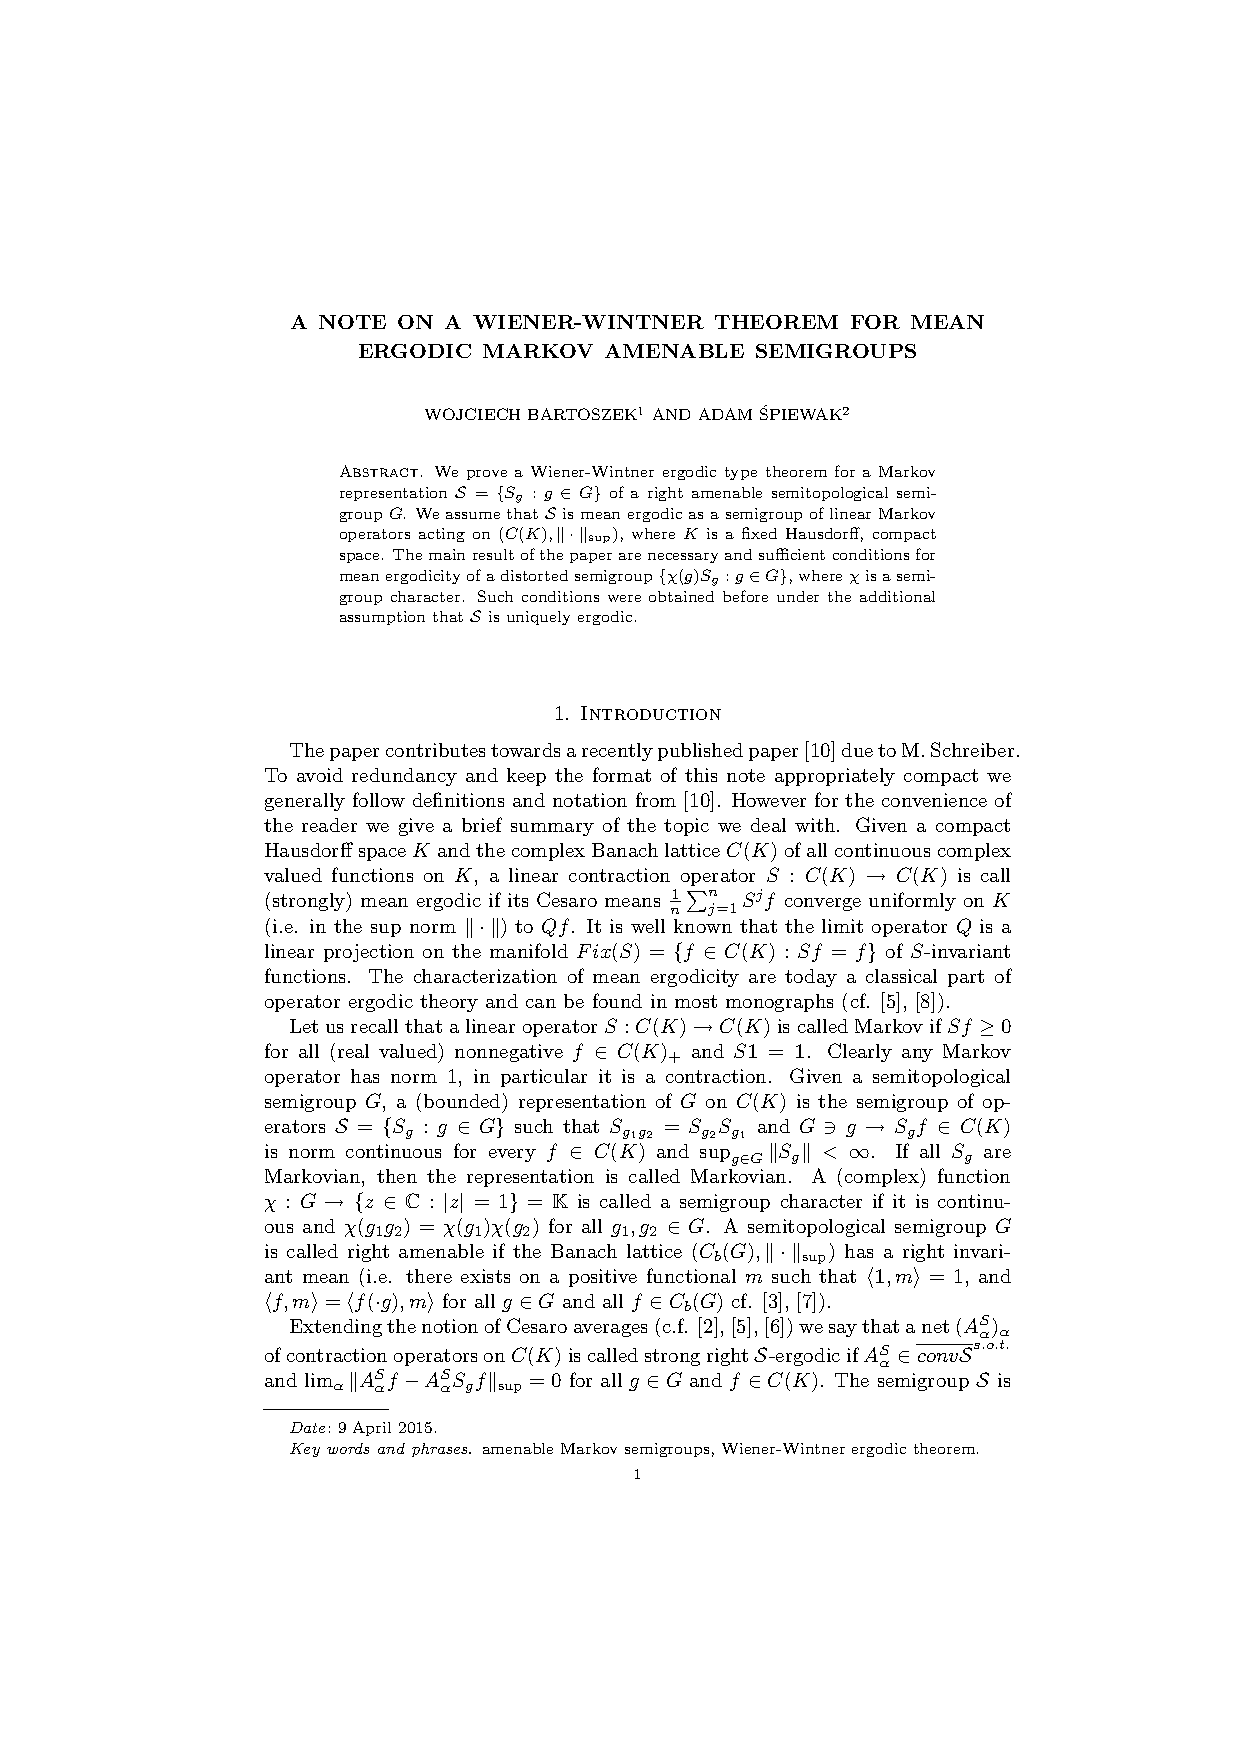
\includepdf[pages=-]{BartoszekSpiewak}
%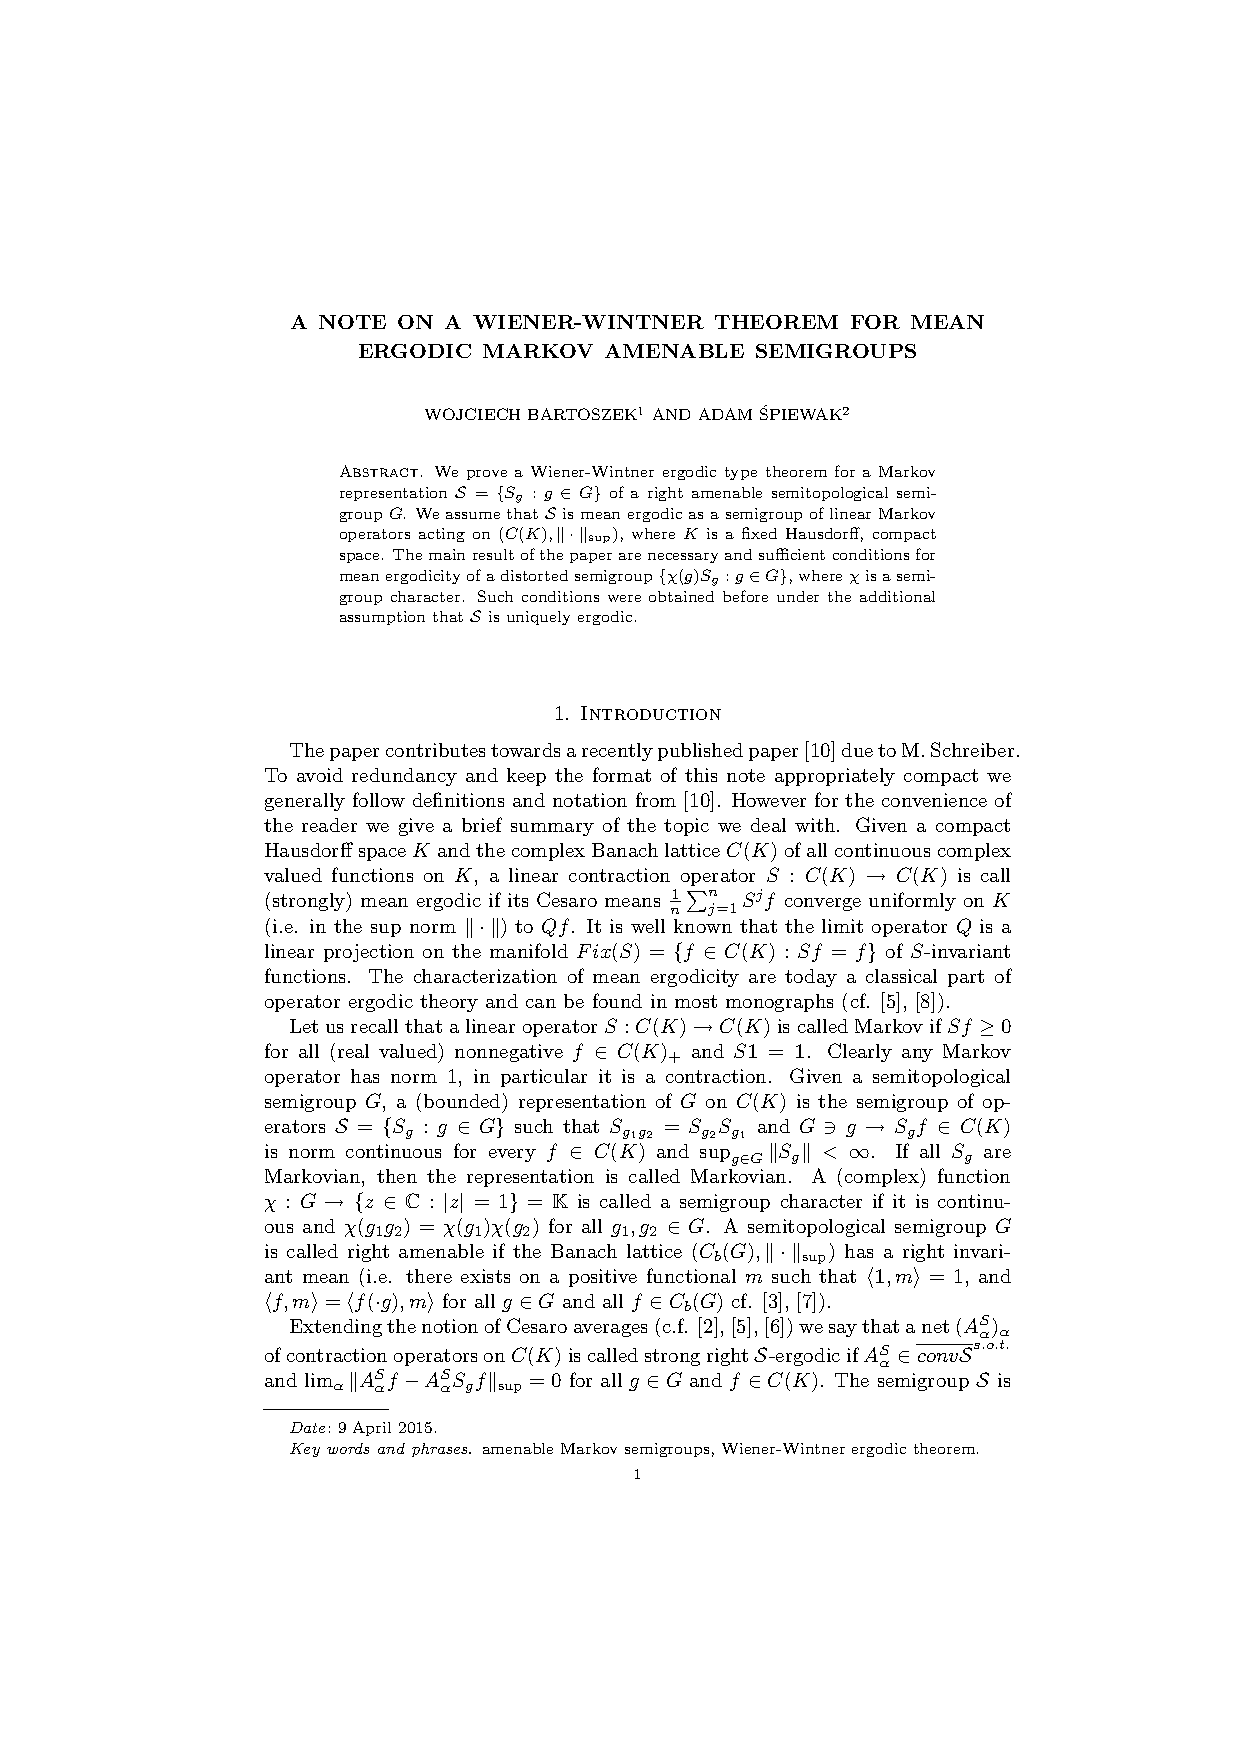
\includepdf[pages=-,pagecommand=]{BartoszekSpiewak.pdf}

\begin{thebibliography}{99}

\addcontentsline{toc}{chapter}{Bibliography}

\bibitem[Assani]{assani} I. Assani,  \textit{Wiener Wintner Ergodic Theorems}, World Scientific, River Edge (2003)

\bibitem[Assani, Presser]{assani_survey} I. Assani, Kimberly Presser, \textit{A Survey of the Return Times Theorem}, arXiv:1209.0856, \url{http://arxiv.org/abs/1209.0856}

\bibitem[Bartoszek, �piewak]{bartoszek} W. Bartoszek, A. �piewak \textit{A note on a Wiener-Wintner theorem for mean ergodic Markov amenable semigroups}, to appear (2015)

\bibitem[Bourgian]{bourgain} J. Bourgain, \textit{Double recurrence and almost sure convergence}, Journal Fur Die Reine Und Angewandte Mathematik 01/1990 (1990)

\bibitem[Einsiedler, Ward]{einsiedler} Manfred Einsiedler, Thomas Ward, \textit{Ergodic Theory with a view towards Number Theory}, Springer, Graduate Texts in Mathematics, Vol. 259

\bibitem[Eisner et al]{eisner} T. Eisner, B. Farkas, M. Haase, R. Nagel, \textit{Operator Theoretic Aspects of
Ergodic Theory}, Graduate Texts in Mathematics, Springer, to appear, \url{http://www.fan.uni-wuppertal.de/fileadmin/mathe/reine_mathematik/funktionalanalysis/farkas/GTM-master-v82.pdf}

\bibitem[Krengel, Brunel]{krengel} Ulrich Krengel, Antoine Brunel, \textit{Ergodic theorems}, Walter de Gruyter, 1985 - 357

\bibitem[Lema�czyk]{lemanczyk} M. Lema�czyk, \textit{Teoria spektralna dla ergodyk�w}, 2010, script, \url{http://www-users.mat.umk.pl/~mlem/files/Teoria_spektralna_dla_ergodykow.pdf}

\bibitem[Robinson]{robinson} E. Arthur Robinson, Jr., \textit{On uniform convergence in the Wiener-Wintner theorem}, J. Lond. Math. Soc. 49
(1994), 493�501.

\bibitem[Rudin1]{rudin} Walter Rudin, \textit{Analiza funkcjonalna}, Wydawnictwo Naukowe PWN, second edition, 2012

\bibitem[Rudin2]{rudin2} Walter Rudin, \textit{Analiza rzeczywista i zespolona}, Wydawnictwo Naukowe PWN, second edition, 2009

\bibitem[Schreiber14]{schreiber14} M. Schreiber, \textit{Topological Wiener - Wintner theorems for amenable operator semigroups}, Ergodic Theory and Dynamical Systems 34 (2014) no. 5, 1674-1698

\bibitem[Schreiber13]{schreiber13} M. Schreiber, \textit{Uniform families of ergodic operator nets},  Semigroup Forum 86 (2013), no. 2, 321-336

\bibitem[Sine]{sine} R. Sine, \textit{Geometric theory of a single Markov operator}, Pacific J. Math. 27 (1968), no. 1, 155-166

\bibitem[Weber]{weber} M. Weber, \textit{Dynamical Systems and Processes}, EMS Publishing House (2009)

\bibitem[WW]{ww} N. Wiener, A. Wintner, \textit{Harmonic Analysis and Ergodic Theory}, American Journal of Mathematics, Vol. 63, No. 2 (Apr., 1941), pp. 415-426

\end{thebibliography}
\end{document}